\documentclass[11pt, oneside, ngerman]{report}

\usepackage[utf8]{inputenc}
\usepackage[T1]{fontenc}
\usepackage[ngerman]{babel}
\usepackage{config/style}
\usepackage{config/code}
\usepackage{glossaries}
\usepackage{biblatex}
\usepackage{booktabs}
\usepackage{array}
\usepackage{amsmath}
\usepackage{tikz}
\usetikzlibrary{shapes.geometric, arrows.meta, positioning, chains, decorations.pathmorphing, patterns}

\addbibresource{references.bib}
\loadglsentries{glossar.tex}

\makeglossaries

\begin{document}

    \newcommand{\paperauthor}{Eric Seidel}
\newcommand{\papersupervisor}{Prof. Luis}
\newcommand{\paperuniversity}{Westfälische Hochschule}

\newcommand{\papertitle}{OPR Semesterzusammenfassung}
\newcommand{\papermajorheading}{OPR}
\newcommand{\paperminorheading}{Alles wichtige auf einen Blick}
    \begin{titlepage}

\newcommand{\HRule}{\rule{\linewidth}{0.5mm}} % Defines a new command for the horizontal lines, change thickness here

\center % Center everything on the page

%----------------------------------------------------------------------------------------
%	HEADING SECTIONS
%----------------------------------------------------------------------------------------

\textsc{\LARGE \paperuniversity}\\[1.0cm] % Name of your university/college
\textsc{\Large \papermajorheading}\\[0.2cm] % Major heading such as course name
\textsc{\large \paperminorheading}\\[0.75cm] % Minor heading such as course title

%----------------------------------------------------------------------------------------
%	TITLE SECTION
%----------------------------------------------------------------------------------------

\HRule \\[0.4cm]
{ \huge \bfseries \papertitle}\\[0.05cm] % Title of your document
\HRule \\[3.5cm]

\begin{center}
	\makebox[0.8\textwidth]{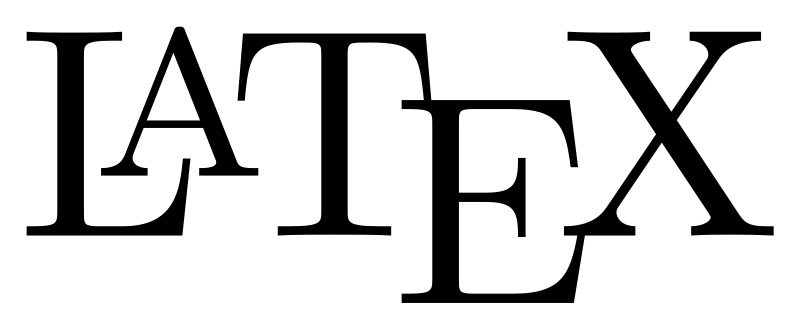
\includegraphics[width=0.8\textwidth]{frontpage.png}}
\end{center}

\vfill % Fill the rest of the page with whitespace

%----------------------------------------------------------------------------------------
%	AUTHOR SECTION
%----------------------------------------------------------------------------------------

\begin{minipage}{0.4\textwidth}
	\begin{flushleft} \large
	\emph{Author(s):}\\
	\paperauthor
	\end{flushleft}
	\end{minipage}
	~
	\begin{minipage}{0.4\textwidth}
	\begin{flushright} \large
	\emph{Supervisor(s):} \\
	\papersupervisor
	\end{flushright}
\end{minipage}\\[1cm]

%----------------------------------------------------------------------------------------
%	DATE SECTION
%----------------------------------------------------------------------------------------

{\large \today}\\ % Date, change the \today to a set date if you want to be precise

\end{titlepage}


    \clearpage
    \thispagestyle{empty}
    \pagenumbering{gobble}

    \renewcommand{\abstractname}{Copyright \textcopyright \xspace \the\year \xspace \paperuniversity}

% \begin{abstract}
\begin{center}

This document, including appendices, is property of \paperuniversity \xspace and is confidential, privileged and only for use of the intended addressees and may not be used, published or redistributed without the prior written consent of \paperuniversity \xspace.

\end{center}
% \end{abstract}

    \renewcommand{\abstractname}{Abstract}

\begin{abstract}
\begin{center}

Lorem ipsum dolor sit amet, consectetur adipiscing elit. Nam a orci ornare nibh tincidunt molestie sed nec tellus. Morbi non sapien id lorem posuere pretium. Vestibulum commodo cursus purus, a elementum sem imperdiet sit amet. Phasellus posuere dolor dignissim aliquam tempus. Morbi egestas felis in lorem varius, ac egestas ante lacinia. Nulla sed ultrices dui. Lorem ipsum dolor sit amet, consectetur adipiscing elit. 

\end{center}
\end{abstract}


    \clearpage
    \pagenumbering{roman} 
    \tableofcontents

    \clearpage
    \pagenumbering{arabic}

    \part{Semesterzusammenfassung}

    \chapter{Pakete in Java}
\label{chap:pakete}

\textit{Pakete schaffen Ordnung.} Sie bilden eine übersichtliche, hierarchische Struktur innerhalb von Java-Projekten.
Im Prinzip sind Pakete Ordnerstrukturen, die Klassen und weitere (Unter-)Pakete enthalten können.
Die Adressierung eines Paketes erfolgt durch seinen vollqualifizierten Paketpfad, der die Hierarchie widerspiegelt:
$p_1.p_2.\dots.p_n$. Dabei ist $p_n$ ein Paket innerhalb von $p_{n-1}$, welches wiederum in $p_{n-2}$ liegt, und so weiter.

Klassen werden analog dazu über ihren vollqualifizierten Namen angesprochen: $p_1.p_2.\dots.p_n.K$, wobei $K$ der Name der Klasse ist.

\begin{lstlisting}[language=Java, caption={Beispiele für Paket- und Klassenspezifikationen}, label=lst:paketbeispiele]
// Paket "regex", enthalten im Paket "util", das im Paket "java" liegt:
java.util.regex

// Klasse "StringTokenizer", enthalten im Paket "util", das im Paket "java" liegt:
java.util.StringTokenizer
\end{lstlisting}

Eine Klasse wird einem spezifischen Paket zugeordnet, indem die \texttt{package}-Anweisung als erste Zeile in der Quelldatei deklariert wird:
\begin{lstlisting}[language=Java, caption={Deklaration der Paketzugehörigkeit}]
package java.util; // Beispielhafter Paketpfad

public class Main {
  // ...
}
\end{lstlisting}
Diese Angabe ist für jede Java-Datei, die zu einem Paket gehört, obligatorisch. Vor der \texttt{package}-Anweisung dürfen lediglich Kommentare stehen
- keine anderen Klassendefinitionen, Variablen oder Importanweisungen.

\section{Importieren von Klassen und Paketen}
\label{sec:importieren}

Um Klassen aus anderen Paketen innerhalb der eigenen Klasse nutzen zu können, müssen diese \textit{importiert} werden.
Die \texttt{import}-Anweisungen stehen dabei stets am Anfang der Datei, nach der optionalen \texttt{package}-Deklaration und 
\textit{vor} dem Klassenkopf (der Klassendefinition).

In modernen Entwicklungsumgebungen (IDEs) werden \texttt{import}-Anweisungen häufig automatisch hinzugefügt oder vorgeschlagen. 
Dennoch kann es in bestimmten Szenarien notwendig sein, diese manuell anzupassen oder zu ergänzen.

\subsection{Importieren aller Klassen eines Pakets (Wildcard-Import)}
\label{ssec:wildcard_import}

Um alle öffentlichen Klassen eines bestimmten Pakets verfügbar zu machen, kann ein sogenannter Wildcard-Import verwendet werden. 
Dieser wird durch das Sternchen (\texttt{*}) symbolisiert. Beispielsweise importiert die Anweisung
\begin{lstlisting}[language=Java, caption={Wildcard-Import des java.util Pakets}]
import java.util.*;
\end{lstlisting}
alle öffentlichen Klassen aus dem Paket \texttt{java.util}. Die importierten Klassen können daraufhin so verwendet werden, 
als wären sie im aktuellen Paket definiert worden.

\paragraph{Vorsicht bei Namenskonflikten:}
Wenn zwei oder mehrere Klassen mit identischem Namen aus unterschiedlichen Paketen importiert werden 
(oder eine importierte Klasse denselben Namen wie eine Klasse im aktuellen Paket hat), entsteht ein Namenskonflikt. 
In solchen Fällen müssen die betroffenen Klassen vollständig Qualifiziert verwendet werden, um Eindeutigkeit zu gewährleisten.
Beispiel:
\begin{lstlisting}[language=Java, caption={Umgang mit Namenskonflikten}]
import java.util.Date;
import java.sql.Date;

public class DateTest {
  java.util.Date utilDate; // Vollständig qualifiziert
  java.sql.Date sqlDate;   // Vollständig qualifiziert

  public void example() {
    utilDate = new java.util.Date(); // Eindeutige Zuweisung
    // Date ambiguDate; // Fehler: Mehrdeutigkeit ohne Qualifizierung
  }
}
\end{lstlisting}

\section{Vollständige Qualifizierung}
Pakete und Klassen, welche über ihren vollen Namen angesprochen werden, nennt man 
\textit{vollständig Qualifiziert}. So wird also anstelle von \lstinline{Date} 
\lstinline{java.util.Date} verwendet. Klassen müssen vollständig Qualifiziert werden,
wenn mehrere Klassen gleich heißen. Beispielsweise \lstinline{java.util.Date} und 
\lstinline{java.sql.Date}. 

\section{Das Paket \texttt{java.lang}}
\label{sec:java_lang}

Das Paket \texttt{java.lang} nimmt eine Sonderstellung ein. Es enthält fundamentale Klassen, die für die grundlegende 
Funktionalität der Java-Sprache unerlässlich sind. Dazu gehören beispielsweise:
\begin{itemize}
    \item \texttt{Object}: Die Wurzelklasse aller Java-Klassen.
    \item \texttt{String}: Für die Verarbeitung von Zeichenketten.
    \item \texttt{System}: Bietet Zugriff auf systemabhängige Ressourcen und Funktionen.
    \item Wrapper-Klassen für primitive Datentypen (z.B. \texttt{Integer}, \texttt{Boolean}).
    \item \texttt{Math}: Stellt mathematische Funktionen bereit.
\end{itemize}
Klassen aus dem \texttt{java.lang}-Paket sind \textbf{immer automatisch verfügbar} und müssen nicht explizit importiert werden.

\subsection{Statische Importanweisungen}
\label{ssec:statische_importe}

Neben dem Import von Klassen ist es auch möglich, statische Methoden und Variablen direkt zu importieren. 
Dies geschieht mithilfe der \texttt{import static}-Anweisung.
Durch einen statischen Import können statische Mitglieder einer Klasse so aufgerufen werden, als wären sie 
in der aktuellen Klasse definiert, ohne den Klassennamen voranstellen zu müssen.

\paragraph{Beispiel für statischen Import:}
Die Anweisung
\begin{lstlisting}[language=Java, caption={Statischer Import der max-Methode}]
import static java.lang.Math.max;
\end{lstlisting}
importiert die statische Methode \texttt{max} aus der Klasse \texttt{Math} (welche sich im Paket \texttt{java.lang} befindet).
Anschließend kann die Methode direkt verwendet werden:
\begin{lstlisting}[language=Java, caption={Verwendung nach statischem Import}]
public class MathExample {
  public int biggerNumber(int a, int b) {
    return max(a, b); // Aufruf ohne "Math." Präfix
  }
}
\end{lstlisting}

Es ist auch möglich, alle statischen Mitglieder einer Klasse zu importieren:
\begin{lstlisting}[language=Java, caption={Statischer Import aller Mitglieder von Math}]
import static java.lang.Math.*;

public class MathExampleAll {
  public double circleSurfaceArea(double radius) {
    return PI * pow(radius, 2); // PI und pow direkt verfügbar
  }
}
\end{lstlisting}

\textbf{Wichtig:} Nicht-statische Variablen oder Methoden können nicht über \texttt{import static} importiert werden. 
Diese Art des Imports ist ausschließlich statischen Mitgliedern vorbehalten. Instanzvariablen (nicht statische Variablen) können
gar nicht importiert werden.

    \chapter{Klassenhierarchie}
\label{chap:klassenhierarchie}

In der objektorientierten Programmierung ermöglicht die Klassenhierarchie die Schaffung von Beziehungen zwischen Klassen, 
wodurch Code-Wiederverwendung gefördert und eine logische Struktur aufgebaut wird. Dieses Kapitel erläutert die fundamentalen 
Konzepte der Vererbung, Sichtbarkeitsmodifikatoren und Bindungsarten in Java.

\section{Vererbung: Das Fundament der Hierarchie}
\label{sec:erben}

Eine Klasse kann Eigenschaften und Methoden von einer anderen Klasse übernehmen. Dieser Mechanismus wird als Vererbung bezeichnet 
und mit dem Schlüsselwort \texttt{extends} realisiert.

\paragraph{Syntax der Vererbung}
Die grundlegende Syntax zur Definition einer Klasse, die von einer anderen erbt, ist wie folgt:
\begin{lstlisting}[language=Java, caption={Deklaration einer abgeleiteten Klasse}]
class Unterklasse extends Oberklasse {
    // Zusätzliche Attribute und Methoden der Unterklasse
    // oder überschriebene Methoden der Oberklasse
}
\end{lstlisting}
In diesem Beispiel ist \texttt{Oberklasse} die direkte Superklasse (auch Elternklasse genannt) von \texttt{Unterklasse}. Umgekehrt ist 
\texttt{Unterklasse} eine direkte Subklasse (auch Kindklasse genannt) von \texttt{Oberklasse}. Eine Klasse kann beliebig viele direkte 
Unterklassen haben, jedoch stets nur \textbf{eine} direkte Oberklasse. Java unterstützt keine Mehrfachvererbung von Klassen. Die Kette 
der Oberklassen bildet die Vererbungshierarchie.

\paragraph{Was wird vererbt?}
Eine Unterklasse erbt von ihrer Oberklasse:
\begin{itemize}
    \item Alle \texttt{public} und \texttt{protected} Instanzmethoden und Klassenmethoden (\texttt{static}).
    \item Alle Instanzvariablen und Klassenvariablen (\texttt{static}). Auch \texttt{private} deklarierte Variablen der Oberklasse sind 
    Teil des Speicherabbilds von Objekten der Unterklasse. Jedoch ist ein direkter Zugriff auf \texttt{private} Variablen der Oberklasse 
    aus der Unterklasse heraus nicht möglich; dieser kann nur über geerbte \texttt{public} oder \texttt{protected} Methoden der Oberklasse 
    erfolgen (Prinzip der Datenkapselung).
\end{itemize}
Die Vererbung ist transitiv: Eine Klasse erbt auch die Member, die ihre Oberklasse bereits von deren Oberklasse geerbt hat. Geerbte Member 
verhalten sich so, als wären sie in der Unterklasse selbst deklariert, sofern sie nicht überschrieben werden.

\paragraph{Erweiterung und Spezialisierung durch die Unterklasse}
Unterklassen können die geerbten Funktionalitäten erweitern und spezialisieren:
\begin{itemize}
    \item Sie können neue Methoden und Variablen definieren, die nur für die Unterklasse spezifisch sind.
    \item Sie können geerbte (nicht-\texttt{final} und nicht-\texttt{private}) Instanzmethoden \textbf{überschreiben} (\texttt{@Override}), 
    um eine spezifische Implementierung bereitzustellen.
\end{itemize}

\paragraph{Nicht vererbte Elemente}
Folgende Elemente werden \textbf{nicht} an Unterklassen vererbt:
\begin{itemize}
    \item \textbf{Konstruktoren:} Jede Klasse muss ihre eigenen Konstruktoren definieren oder den Default-Konstruktor verwenden. Der Konstruktor 
    der Oberklasse kann jedoch mittels \texttt{super()} aufgerufen werden (siehe Abschnitt~\ref{sec:super}).
    \item \textbf{Private Methoden:} Private Methoden der Oberklasse sind für die Unterklasse unsichtbar und werden daher nicht vererbt. Folglich 
    können sie auch nicht im Sinne der Polymorphie überschrieben werden. Definiert eine Unterklasse eine Methode mit derselben Signatur wie eine 
    private Methode der Oberklasse, so handelt es sich um eine vollkommen neue, unabhängige Methode. Es besteht keine polymorphe Beziehung zwischen 
    diesen beiden Methoden; die Methode in der Unterklasse \textit{verdeckt} (shadows) lediglich die Methode der Oberklasse, falls diese z.B. über 
    einen Cast auf den Oberklassentyp aufgerufen würde (was bei privaten Methoden aber ohnehin nicht direkt von außen geht).
\end{itemize}

\subsection{Der Sichtbarkeitsmodifikator \texttt{protected}}
\label{ssec:protected}

Der Modifikator \texttt{protected} stellt eine Sichtbarkeitsstufe zwischen \texttt{public} und \texttt{private} dar. Mit \texttt{protected} deklarierte 
Member (Methoden oder Variablen) sind sichtbar:
\begin{itemize}
    \item Innerhalb der eigenen Klasse.
    \item Innerhalb aller Unterklassen, auch wenn diese sich in anderen Paketen befinden.
    \item Innerhalb aller anderen Klassen desselben Pakets.
\end{itemize}
Obwohl \texttt{protected} für Instanzvariablen in Vererbungsszenarien nützlich erscheinen mag, sollten Instanzvariablen aus Gründen der Kapselung 
und Wartbarkeit in den meisten Fällen als \texttt{private} deklariert werden. Der Zugriff sollte dann über \texttt{public} oder \texttt{protected} 
Getter- und Setter-Methoden erfolgen.

\subsection{Bindung von Methodenaufrufen: Statisch vs. Dynamisch}
\label{ssec:bindungen}

Die Bindung legt fest, welche konkrete Methodenimplementierung bei einem Aufruf ausgeführt wird.

\paragraph{Statische Bindung (Early Binding)}
Bei der statischen Bindung wird bereits zur Kompilierzeit festgelegt, welche Methodenimplementierung ausgeführt wird. Dies geschieht typischerweise für:
\begin{itemize}
    \item \texttt{private}-Methoden
    \item \texttt{static}-Methoden
    \item \texttt{final}-Instanzmethoden
    \item Aufrufe mit \texttt{super.}
    \item Aufrufe, bei denen der Compiler den exakten Objekttyp eindeutig bestimmen kann.
\end{itemize}

\begin{lstlisting}[language=Java, caption={Beispiele für statische Bindung}]
class Vehicle {
  public static String getCategorie() {
    return "Allgemeines Fahrzeug";
  }
  public final void startMotor() {
    System.out.println("Motor gestartet (finale Methode aus Fahrzeug)");
  }
}

class Car extends Vehicle {
  // Diese Methode verdeckt getCategorie() von Fahrzeug, überschreibt sie aber nicht.
  public static String getCategorie() {
    return "Automobil";
  }
}

public class TestBinding {
  public static void main(String[] args) {
    // Aufruf statischer Methoden: Immer statische Bindung
    System.out.println(Vehicle.getCategorie()); // Gibt "Allgemeines Fahrzeug" aus
    System.out.println(Car.getCategorie());     // Gibt "Automobil" aus

    Car meinAuto = new Car();
    // Aufruf einer finalen Methode: Statische Bindung
    meinAuto.startMotor(); // Ruft Vehicle.startMotor()

    Vehicle meinFahrzeug = new Car();
    // Obwohl meinFahrzeug auf ein Car-Objekt zeigt, wird bei statischen Methoden
    // der deklarierte Typ der Referenz (Car) für die Bindung verwendet.
    // System.out.println(meinFahrzeug.getCategorie()); // Schlechter Stil! Sollte Vehicle.getCategorie() sein.
    // Würde "Allgemeines Fahrzeug" ausgeben.
  }
}
\end{lstlisting}

\paragraph{Dynamische Bindung (Late Binding)}
Bei der dynamischen Bindung wird erst zur Laufzeit entschieden, welche Methodenimplementierung ausgeführt wird. Dies ist 
das Kernprinzip der Polymorphie und tritt bei überschriebenen Instanzmethoden auf. Der Java Virtual Machine (JVM) ermittelt 
den tatsächlichen Typ des Objekts, auf dem die Methode aufgerufen wird, und wählt die entsprechende Implementierung aus.

\begin{lstlisting}[language=Java, caption={Beispiel für dynamische Bindung}]
class Animal {
  public void say() {
    System.out.println("Ein Tier gibt einen Laut von sich.");
  }
}

class Dog extends Animal {
  @Override
  public void say() {
    System.out.println("Wuff! Wuff!");
  }
}

class Cat extends Animal {
  @Override
  public void say() {
    System.out.println("Miau!");
  }
}

public class Zoo {
  public static void main(String[] args) {
    Animal[] tiere = new Animal[3];
    tiere[0] = new Dog();       // Hund-Objekt
    tiere[1] = new Cat();       // Katze-Objekt
    tiere[2] = new Animal();    // Tier-Objekt

    for (Tier aktuellesTier : tiere) {
      // Dynamische Bindung:
      // Zur Laufzeit wird die spezifische say()-Methode
      // des tatsächlichen Objekttyps aufgerufen.
      aktuellesTier.say();
    }
    // Ausgabe:
    // Wuff! Wuff!
    // Miau!
    // Ein Tier gibt einen Laut von sich.
  }
}
\end{lstlisting}
Der Compiler prüft lediglich, ob eine Methode \texttt{say()} im deklarierten Typ \texttt{Animal} existiert. Welche konkrete 
Implementierung dann ausgeführt wird, entscheidet die JVM basierend auf dem Laufzeittyp des Objekts in \texttt{aktuellesTier}.

\section{Das Schlüsselwort \texttt{super} (Prüfungsrelevant!)}
\label{sec:super}

Das Schlüsselwort \texttt{super} hat in Java zwei primäre Verwendungszwecke im Kontext der Vererbung:
\begin{enumerate}
    \item Aufruf des Konstruktors der direkten Oberklasse.
    \item Zugriff auf Member (Methoden oder Variablen) der Oberklasse, die in der aktuellen Klasse möglicherweise überschrieben oder verdeckt wurden.
\end{enumerate}

\paragraph{Aufruf des Oberklassen-Konstruktors mit \texttt{super()}}
Der Aufruf \texttt{super()} dient dazu, einen Konstruktor der direkten Oberklasse explizit auszuführen.
\begin{itemize}
    \item Dieser Aufruf \textbf{muss}, falls vorhanden, die \textbf{erste Anweisung} im Konstruktor der Unterklasse sein.
    \item Die Parameterliste von \texttt{super(...)} muss mit der Signatur eines Konstruktors der Oberklasse übereinstimmen.
\end{itemize}

\begin{lstlisting}[language=Java, caption={Expliziter Aufruf des Oberklassen-Konstruktors via \texttt{super()}}]
class BaseClass {
  String name;
  public BaseClass(String name) {
    this.name = name;
    System.out.println("Konstruktor Basisklasse aufgerufen mit: " + name);
  }
  public BaseClass() {
    this.name = "Default";
    System.out.println("Parameterloser Konstruktor Basisklasse aufgerufen");
  }
}

class ChildClass extends BaseClass {
  public ChildClass(String spezifischerName) {
    super(spezifischerName); // Ruft BaseClass(String name) auf
    System.out.println("Konstruktor ChildClass aufgerufen");
  }
  public ChildClass() {
    super(); // Ruft BaseClass() auf
    // Alternativ: super("DefaultAbgeleitet");
    System.out.println("Parameterloser Konstruktor ChildClass aufgerufen");
  }
}

public class TestSuper {
  public static void main(String[] args) {
    ChildClass obj = new ChildClass("TestObjekt");
    // Ausgabe:
    // Konstruktor BaseClass aufgerufen mit: TestObjekt
    // Konstruktor ChildClass aufgerufen

    ChildClass obj2 = new ChildClass();
    // Ausgabe:
    // Parameterloser Konstruktor BaseClass aufgerufen
    // Parameterloser Konstruktor ChildClass aufgerufen
  }
}
\end{lstlisting}

\paragraph{Impliziter Aufruf von \texttt{super()}}
Wenn im Konstruktor einer Unterklasse \textbf{kein expliziter Aufruf} von \texttt{super(...)} (oder \texttt{this(...)}, siehe unten) 
als erste Anweisung steht, fügt der Java-Compiler automatisch einen parameterlosen Aufruf \texttt{super();} ein.
\begin{itemize}
    \item Dies gilt auch für Klassen, die nicht explizit von einer anderen Klasse erben - diese erben implizit von der 
    Klasse \texttt{Object}, die einen parameterlosen Konstruktor besitzt.
    \item Wenn eine Klasse gar keinen Konstruktor definiert, fügt der Compiler einen öffentlichen, parameterlosen Default-Konstruktor 
    ein, der ebenfalls implizit \texttt{super();} aufruft.
\end{itemize}

\begin{lstlisting}[language=Java, caption={Impliziter Konstruktor und \texttt{super()}-Aufruf durch den Compiler}]
class Ober {
  public Ober() {
    System.out.println("Konstruktor Ober");
  }
}

class Unter extends Ober {
  // Kein expliziter Konstruktor definiert
}
// Der Compiler generiert für Klasse Unter:
// public Unter() {
//   super(); // Impliziter Aufruf des Ober-Konstruktors
// }

public class TestImplizit {
  public static void main(String[] args) {
    Unter u = new Unter(); // Führt zu Ausgabe: "Konstruktor Ober"
  }
}
\end{lstlisting}

\paragraph{Kompilierfehler bei fehlendem passenden Oberklassen-Konstruktor}
Der implizite \texttt{super();}-Aufruf (oder ein expliziter ohne Argumente) funktioniert nur, wenn die direkte Oberklasse einen 
zugänglichen, parameterlosen Konstruktor besitzt. Ist dies nicht der Fall (z.B. weil die Oberklasse nur Konstruktoren mit Parametern definiert), 
\textbf{muss} die Unterklasse in jedem ihrer Konstruktoren explizit einen passenden Konstruktor der Oberklasse mittels \texttt{super(...)} mit 
den erforderlichen Argumenten aufrufen. Andernfalls entsteht ein Kompilierfehler. Der Compiler kann die benötigten Argumente nicht "erraten".

\begin{lstlisting}[language=Java, caption={Kompilierfehler: \texttt{super()}-Aufruf scheitert bei parametrisiertem Superkonstruktor}]
class Elternteil {
  private final String id;
  public Elternteil(String id) { // Nur ein Konstruktor mit Parameter
    this.id = id;
  }
}

class KindValid extends Elternteil {
  public KindValid(String kindId, String elternId) {
        super(elternId); // Korrekt: Expliziter Aufruf des passenden Konstruktors
  }
}

class KindError1 extends Elternteil {
  public KindError1() {
    // FEHLER! Implizites super() würde Elternteil() suchen, gibt es aber nicht.
    // Explizites super("someID") wäre nötig.
  }
}

class KindError2 extends Elternteil {
  // FEHLER! Compiler fügt Default-Konstruktor ein, der super() aufruft.
  // Elternteil() existiert nicht.
}
\end{lstlisting}

\paragraph{Zugriff auf Member der Oberklasse mit \texttt{super.}}
Mit \texttt{super.methodenName()} oder \texttt{super.variablenName} kann auf eine Methode oder Variable der Oberklasse zugegriffen werden, 
selbst wenn diese in der aktuellen Klasse überschrieben (Methode) oder verdeckt (Variable) wurde. Dies ist nützlich, um die Funktionalität 
der Oberklasse zu erweitern, anstatt sie komplett zu ersetzen.

\begin{lstlisting}[language=Java, caption={Zugriff auf überschriebene Methode der Oberklasse via \texttt{super.}}]
class Basis {
  public void anzeige() {
    System.out.println("Anzeige aus Basis");
  }
  protected String info = "Info aus Basis";
}

class Erweitert extends Basis {
  @Override
  public void anzeige() {
    super.anzeige(); // Ruft anzeige() der Klasse Basis auf
    System.out.println("Anzeige aus Erweitert");
  }
    
  public void zeigeInfos() {
    System.out.println("Eigene Info: " + this.info); // this.info ist hier redundant, da info nicht neu deklariert wurde
    System.out.println("Basis Info: " + super.info); // Greift auf info der Basisklasse zu
  }

  // Beispiel für Variablenverdeckung (Shadowing) - generell vermeiden!
  // protected String info = "Info aus Erweitert"; 
  // public void zeigeInfosMitVerdeckung() {
  //     System.out.println("Eigene Info (verdeckt): " + this.info); // Info aus Erweitert
  //     System.out.println("Basis Info (via super): " + super.info); // Info aus Basis
  // }
}

public class TestSuperMember {
  public static void main(String[] args) {
    Erweitert ext = new Erweitert();
    ext.anzeige();
    // Ausgabe:
    // Anzeige aus Basis
    // Anzeige aus Erweitert
    ext.zeigeInfos();
  }
}
\end{lstlisting}


\section{Konstruktoraufrufe mit \texttt{this()}}
\label{sec:this_konstruktor}

Analog zum Aufruf eines Oberklassen-Konstruktors mit \texttt{super()} kann mit \texttt{this()} ein anderer Konstruktor derselben 
Klasse aufgerufen werden. Dies wird als Konstruktorverkettung (constructor chaining) bezeichnet und dient dazu, Code-Duplizierung 
innerhalb verschiedener Konstruktoren einer Klasse zu vermeiden.
\begin{itemize}
    \item Der Aufruf \texttt{this(...)} \textbf{muss}, falls vorhanden, die \textbf{erste Anweisung} im Konstruktor sein.
    \item Ein Konstruktor kann entweder einen \texttt{super(...)} oder einen \texttt{this(...)} Aufruf als erste Anweisung enthalten, aber nicht beide.
    \item Mindestens ein Konstruktor in der Kette muss (implizit oder explizit) den Konstruktor der Oberklasse via \texttt{super(...)} aufrufen.
\end{itemize}

\begin{lstlisting}[language=Java, caption={Aufruf eines anderen Konstruktors derselben Klasse via \texttt{this()}}]
class Benutzer {
  private final String benutzername;
  private final String email;
  private boolean istAktiv;

  public Benutzer(String benutzername, String email) {
    this.benutzername = benutzername;
    this.email = email;
    this.istAktiv = true; // Standardwert
    System.out.println("Benutzer erstellt: " + benutzername + ", Aktiv: " + istAktiv);
  }

  public Benutzer(String benutzername) {
    this(benutzername, benutzername + "@example.com"); // Ruft den ersten Konstruktor auf
    System.out.println("Benutzer (nur Name) erstellt, E-Mail generiert.");
  }
    
  public Benutzer() {
    this("gast"); // Ruft den zweiten Konstruktor auf, der dann den ersten aufruft
    this.istAktiv = false; // Überschreibt den Standardwert für Gast-Benutzer
    System.out.println("Gast-Benutzer erstellt, Inaktiv gesetzt.");
  }
}

public class TestThisKonstruktor {
  public static void main(String[] args) {
    Benutzer b1 = new Benutzer("alice", "alice@mail.com");
    System.out.println("---");
    Benutzer b2 = new Benutzer("bob");
    System.out.println("---");
    Benutzer b3 = new Benutzer();
  }
}
\end{lstlisting}

\section{Finale Klassen und Methoden}
\label{sec:final}

Das Schlüsselwort \texttt{final} hat im Kontext der Vererbung spezielle Bedeutungen:

\paragraph{Finale Klassen}
Eine mit \texttt{final} deklarierte Klasse \textbf{kann nicht erweitert werden}, d.h., es können keine Unterklassen von ihr abgeleitet werden.
\begin{lstlisting}[language=Java, caption={\texttt{final} Klasse}]
public final class Unveraenderlich {
  // ...
}

// class VersuchAbleitung extends Unveraenderlich { } // KOMPILIERFEHLER!
\end{lstlisting}
Dies wird oft für Klassen verwendet, deren Implementierung als abgeschlossen und nicht für Erweiterungen vorgesehen gilt (z.B. \texttt{String} oder \texttt{Integer}).

\paragraph{Finale Methoden}
Eine mit \texttt{final} deklarierte Methode \textbf{kann in Unterklassen nicht überschrieben werden}.
\begin{lstlisting}[language=Java, caption={\texttt{final} Methode}]
class BasisMitFinal {
  public final void wichtigeOperation() {
    System.out.println("Diese Operation darf nicht geändert werden.");
  }
  public void andereOperation() {
    System.out.println("Diese Operation kann überschrieben werden.");
  }
}

class AbgeleitetVonFinal extends BasisMitFinal {
  // @Override
  // public final void wichtigeOperation() { } // KOMPILIERFEHLER!

  @Override
  public void andereOperation() {
    System.out.println("andereOperation in AbgeleitetVonFinal überschrieben.");
  }
}
\end{lstlisting}
Finale Methoden garantieren, dass das Verhalten dieser spezifischen Methode in der gesamten Klassenhierarchie unterhalb 
ihrer Definition konstant bleibt. Sie werden auch vom Compiler für Optimierungen herangezogen, da die Bindung statisch erfolgen kann.


    \chapter{JUnit Tests (Sehr Prüfungsrelevant)}

JUnit Tests sind ein fundamentaler Bestandteil der modernen Softwareentwicklung und ein häufiges Thema in Prüfungen. Dieses Kapitel führt in die Grundlagen des Testens mit JUnit ein.

\section{Hintergrund von Tests}
Software zu testen ist unerlässlich, um deren korrekte Funktionalität sicherzustellen. Eine bewährte Praxis ist das Test-Driven Development (TDD), bei dem Tests vor der eigentlichen Implementierung der Anwendungslogik geschrieben werden. Tests definieren die Anforderungen an das Programm und dienen als ausführbare Spezifikation. Testfälle repräsentieren dabei konkrete Anwendungsszenarien.

\section{Tests schreiben mit JUnit}
Testklassen in JUnit dienen dazu, die Methoden einer Anwendungsklasse systematisch zu überprüfen. Idealerweise existiert für jede Anwendungsklasse eine korrespondierende Testklasse. Diese Testklassen bündeln Testmethoden, die einzelne Aspekte oder Testfälle der zu testenden Methoden abdecken. Es ist üblich und empfehlenswert, mehrere Testmethoden für eine einzelne Anwendungsmethode zu erstellen, um verschiedene Szenarien (z.B. Normalfall, Grenzfälle, Fehlerfälle) abzudecken. Testmethoden sollten voneinander unabhängig sein und isoliert ausgeführt werden können.

\subsection{Importe für JUnit}
Für die Verwendung von JUnit müssen spezifische Annotationen und Assertions-Methoden importiert werden. JUnit ist ein weit verbreitetes Framework für das Testen von Java-Code.

\begin{lstlisting}[language=Java, caption={Grundlegende JUnit 5 Importe}, label=lst:junit_imports, basicstyle=\ttfamily\footnotesize, breaklines=true, frame=tb, numbers=left]
// Annotationen für Test-Setup und Testmethoden
import org.junit.jupiter.api.BeforeEach; // Wird vor jeder Testmethode ausgeführt
import org.junit.jupiter.api.AfterEach;  // Wird nach jeder Testmethode ausgeführt (seltener benötigt)
import org.junit.jupiter.api.Test;       // Markiert eine Methode als Testmethode
import org.junit.jupiter.api.Disabled;   // Deaktiviert eine Testmethode oder -klasse

// Statische Importe für Assertions-Methoden (empfohlen für bessere Lesbarkeit)
import static org.junit.jupiter.api.Assertions.assertEquals;
import static org.junit.jupiter.api.Assertions.assertTrue;
import static org.junit.jupiter.api.Assertions.assertFalse;
import static org.junit.jupiter.api.Assertions.assertNull;
import static org.junit.jupiter.api.Assertions.assertNotNull;
import static org.junit.jupiter.api.Assertions.assertThrows;
// Es gibt viele weitere Assertions-Methoden in org.junit.jupiter.api.Assertions
\end{lstlisting}
Hinweis: Die Verwendung von \textit{AfterEach} ist seltener notwendig als \textit{BeforeEach}, da gut designte Tests oft keine explizite Aufräumarbeit nach jedem Test benötigen (z.B. wenn keine externen Ressourcen geöffnet werden).

\subsection{Struktur einer Testklasse}
\label{ssec:junit_klassenkopf}
Gemäß der Namenskonvention sollte eine Testklasse für eine Klasse `MyClass` den Namen `MyClassTest` tragen. Instanzvariablen in Testklassen sind üblich, um Testobjekte oder Testdaten zu halten, die von mehreren Testmethoden verwendet werden. Um die Unabhängigkeit der Tests zu gewährleisten, sollten diese Instanzvariablen typischerweise in einer mit `@BeforeEach` annotierten Methode `setUp()` vor jeder Testmethode neu initialisiert werden.

\begin{lstlisting}[language=Java, caption={Grundgerüst einer JUnit Testklasse}, label=lst:junit_test_class_structure, basicstyle=\ttfamily\footnotesize, breaklines=true, frame=tb, numbers=left]
// Angenommen, wir testen eine Klasse namens "Calculator"
class CalculatorTest {

    private Calculator calculatorInstance; // Instanzvariable für das Testobjekt

    @BeforeEach
    void setUp() {
        // Diese Methode wird vor jeder @Test Methode ausgeführt.
        // Ideal für die Initialisierung von Testobjekten.
        calculatorInstance = new Calculator();
        System.out.println("setUp() executed: New Calculator instance created.");
    }

    @AfterEach
    void tearDown() {
        // Diese Methode wird nach jeder @Test Methode ausgeführt.
        // Nützlich für Aufräumarbeiten, z.B. Schließen von Ressourcen.
        // In vielen Fällen nicht zwingend notwendig.
        calculatorInstance = null; // Beispiel: Objekt freigeben
        System.out.println("tearDown() executed.");
    }

    @Test
    void testAddition() {
        // Testlogik für die Additionsmethode
        int result = calculatorInstance.add(5, 3);
        assertEquals(8, result, "5 + 3 should be 8"); // Assertion mit optionaler Nachricht
    }

    @Test
    void testSubtraction() {
        // Testlogik für die Subtraktionsmethode
        int result = calculatorInstance.subtract(10, 4);
        assertEquals(6, result, "10 - 4 should be 6");
    }
    
    @Test
    @Disabled("This test is currently disabled due to ongoing refactoring.")
    void testMultiplication() {
        // Ein deaktivierter Test
        assertEquals(12, calculatorInstance.multiply(3,4));
    }
}

// Dummy-Klasse, die getestet wird (normalerweise in einer separaten Datei)
class Calculator {
    public int add(int a, int b) { return a + b; }
    public int subtract(int a, int b) { return a - b; }
    public int multiply(int a, int b) { return a * b; }
}
\end{lstlisting}

\subsection{Testdaten initialisieren mit \texttt{@BeforeEach}}
\label{ssec:junit_beforeeach}
Um sicherzustellen, dass jede Testmethode mit einem sauberen und definierten Zustand startet, werden Testdaten und -objekte häufig in einer Methode initialisiert, die mit `@BeforeEach` annotiert ist. Die Namenskonvention für diese Methode ist `setUp()`.

\begin{lstlisting}[language=Java, caption={Verwendung von \texttt{@BeforeEach} zur Initialisierung}, label=lst:junit_beforeeach_example, basicstyle=\ttfamily\footnotesize, breaklines=true, frame=tb, numbers=left]
class Book { // Beispielklasse, die getestet wird
    private String title;
    private String author;
    // Weitere Attribute und Konstruktor...
    public Book(String title, String author) { this.title = title; this.author = author; }
    public String getAsText() { return title + "; " + author; }
}

class BookTest {
    private Book testBook; // Instanzvariable für das Testobjekt

    @BeforeEach
    void setUp() {
        // Initialisiert das testBook Objekt vor jedem Test neu
        testBook = new Book("The Hitchhiker's Guide to the Galaxy", "Douglas Adams");
    }

    @Test
    void testBookCreation() {
        assertNotNull(testBook, "Book should be initialized by setUp()");
    }

    @Test
    void testGetAsText() {
        String expectedText = "The Hitchhiker's Guide to the Galaxy; Douglas Adams";
        assertEquals(expectedText, testBook.getAsText(), "getAsText() should return correct format.");
    }
}
\end{lstlisting}

\subsection{Testdaten abbauen mit \texttt{@AfterEach} (seltener)}
\label{ssec:junit_aftereach}
Falls nach der Ausführung jeder Testmethode Aufräumarbeiten notwendig sind (z.B. das Schließen von Dateien, Netzwerkverbindungen oder das Zurücksetzen von globalen Zuständen), kann dies in einer mit `@AfterEach` annotierten Methode geschehen. Die Namenskonvention hierfür ist `tearDown()`. Für die meisten Unit-Tests, die mit einfachen Objekten arbeiten, ist dies nicht erforderlich.

\begin{lstlisting}[language=Java, caption={Verwendung von \texttt{@AfterEach} für Aufräumarbeiten}, label=lst:junit_aftereach_example, basicstyle=\ttfamily\footnotesize, breaklines=true, frame=tb, numbers=left]
// @AfterEach // Selten benötigt für einfache Unit-Tests
// void tearDown() {
//     // Diese Methode wird nach jedem Testfall aufgerufen.
//     // Beispiel: Schließen einer Datei, Freigeben von Ressourcen.
//     // System.out.println("tearDown() called.");
// }
\end{lstlisting}

\subsection{Testmethoden und Assertions}
\label{ssec:junit_testmethoden}
Testmethoden werden mit `@Test` annotiert. Die Namenskonvention für Testmethoden ist oft `test<MethodenNameDieGetestetWird>[_Szenario]`, z.B. `testAdd_withPositiveNumbers` oder `testAdd_withNegativeNumbers`. Testmethoden haben in der Regel keine Rückgabewerte (`void`) und keine Modifikatoren (package-private Sichtbarkeit ist üblich). Sie sollten prägnant sein und sich auf die Überprüfung eines spezifischen Aspekts konzentrieren.

Innerhalb einer Testmethode werden Assertions verwendet, um das tatsächliche Verhalten des Codes mit dem erwarteten Verhalten zu vergleichen.
\begin{lstlisting}[language=Java, caption={Beispiel einer Testmethode mit Assertions}, label=lst:junit_testmethod_example, basicstyle=\ttfamily\footnotesize, breaklines=true, frame=tb, numbers=left]
// Innerhalb einer Testklasse, z.B. BookTest (siehe oben)

// @BeforeEach
// void setUp() {
//     testBook = new Book("Asterix der Gallier", "Uderzo", 1965, 9.8);
// }

// Angenommen, die Book-Klasse hat eine Methode getFormattedString():
// public String getFormattedString() {
//     return String.format("%s; %s; %d; %.1f", title, author, year, price);
// }
// Und der Konstruktor ist: public Book(String title, String author, int year, double price)

// @Test
// void testGetFormattedString_validBook() {
//     // Annahme: testBook wurde in setUp() initialisiert
//     // testBook = new Book("Asterix der Gallier", "Uderzo", 1965, 9.8); // Falls kein setUp
//     String expectedOutput = "Asterix der Gallier; Uderzo; 1965; 9.8";
//     // assertEquals(expectedOutput, testBook.getFormattedString());
// }
\end{lstlisting}
In diesem Beispiel würde `assertEquals` prüfen, ob der von `book.getFormattedString()` zurückgegebene String dem `expectedOutput` entspricht. Die `equals`-Methode des Vergleichsobjekts wird hierfür herangezogen (für Strings ist dies ein Inhaltsvergleich).

Einige gängige Assertions sind:
\begin{itemize}
    \item \texttt{assertEquals(expected, actual, [message])}: Überprüft, ob zwei Werte gleich sind.
    \item \texttt{assertTrue(condition, [message])}: Überprüft, ob eine Bedingung wahr ist.
    \item \texttt{assertFalse(condition, [message])}: Überprüft, ob eine Bedingung falsch ist.
    \item \texttt{assertNull(object, [message])}: Überprüft, ob ein Objekt \texttt{null} ist.
    \item \texttt{assertNotNull(object, [message])}: Überprüft, ob ein Objekt nicht \texttt{null} ist.
    \item \texttt{assertArrayEquals(expectedArray, actualArray, [message])}: Vergleicht zwei Arrays auf Gleichheit (Element für Element).
    \item \texttt{assertThrows(expectedThrowable, executable, [message])}: Überprüft, ob die Ausführung des `executable` Codes eine Exception vom Typ `expectedThrowable` wirft.
\end{itemize}
Die optionale `message` wird angezeigt, wenn die Assertion fehlschlägt, was die Fehlersuche erleichtert.

\subsection{Mock-Klassen zum Testen abstrakter Klassen oder Abhängigkeiten}
\label{ssec:junit_mock_klassen}
Um abstrakte Klassen zu testen oder Klassen, die komplexe Abhängigkeiten haben, werden oft Mock-Klassen (oder Mock-Objekte) verwendet. Eine Mock-Klasse ist eine vereinfachte Implementierung einer Abhängigkeit, die speziell für Testzwecke erstellt wird. Sie simuliert das Verhalten der echten Abhängigkeit in einer kontrollierten Weise.
Die Namenskonvention für eine Mock-Klasse für `AbstractDataProvider` könnte `MockAbstractDataProvider` oder `TestDataProviderImpl` sein.

\begin{lstlisting}[language=Java, caption={Konzept einer Mock-Klasse (vereinfacht)}, label=lst:junit_mock_concept, basicstyle=\ttfamily\footnotesize, breaklines=true, frame=tb, numbers=left]
// Abstrakte Klasse, die getestet werden soll (indirekt)
abstract class AbstractDataProcessor {
    protected abstract String fetchData(); // Abhängigkeit, die gemockt werden könnte

    public String processData() {
        String data = fetchData();
        return "Processed: " + data.toUpperCase();
    }
}

// Eine konkrete Implementierung der abstrakten Klasse für Testzwecke (eine Art Mock)
class TestableDataProcessor extends AbstractDataProcessor {
    private String dataToReturn;

    public TestableDataProcessor(String dataToReturn) {
        this.dataToReturn = dataToReturn;
    }

    @Override
    protected String fetchData() {
        // Simuliert das Verhalten der Abhängigkeit
        return this.dataToReturn;
    }
}

// Testklasse
class AbstractDataProcessorTest {
    @Test
    void testProcessData_withMockedData() {
        // Erstellt eine Instanz der Test-Implementierung mit kontrollierten Daten
        AbstractDataProcessor processor = new TestableDataProcessor("sample data");
        String result = processor.processData();
        assertEquals("Processed: SAMPLE DATA", result);
    }
}
\end{lstlisting}
Für komplexere Mocking-Szenarien werden oft Mocking-Frameworks wie Mockito oder EasyMock eingesetzt, die das Erstellen und Konfigurieren von Mock-Objekten erheblich vereinfachen. Diese sind jedoch über den Rahmen dieser Einführung hinausgehend.


    \chapter{Klasse Object}
\label{chap:Klasse Object}

Die klasse Object ist eine besondere Klasse. \textit{jede} Klasse erbt von der
Object Klasse. In der Object Klasse sind einige Methoden definiert, welche jede
Klasse besitzt. Zu ihnen gehöhren beispielsweise
\lstinline{equals} und \lstinline{hashcode}

\subsection{equals und hashcode}

Die \lstinline{equals} und \lstinline{hashcode} Methoden haben einen Vertrag.
Wenn eine von beiden überschrieben wird, muss die andere auch überschrieben
werden. Wenn Objekte im sinne von
\lstinline{equals} gleich sind, \textit{müssen} diese auch den selben
\lstinline{hashcode} besitzen. Wenn objekte jedoch den selben \lstinline{hashcode}
haben, müssen sie nicht zwingend im sinne von \lstinline{equals} gleich sein.

Standardmäßig prüft die
\lstinline{equals} methode auf gleichheit der Identität, die \lstinline{hashcode}
methode gibt die memory addresse zurück.

\subsection{toString}

Das Objekt wird textuell ausgegeben. Diese Methode wird beispielsweise
aufgerufen, wenn ein Objet über ein \lstinline{System.out.println} in die
Konsole ausgegeben wird.

Die Klasse Objekt hat noch viele weitere Methoden implementiert, allerdings
sind keien weiteren Prüfungsrelevant.
    \chapter{Collection-Klassen}
\label{chap:CollectionKlassen}

Arrays haben eine feste Größe, die sich während der Laufzeit nicht ändern kann. Dies stellt häufig eine Einschränkung dar. Sogenannte Collection-Klassen (oder Kollektionen) bieten hier flexiblere Alternativen. Es gibt verschiedene Arten von Collection-Klassen, die sich grob in Listen (\texttt{List}), Mengen (\texttt{Set}) und Abbildungen (\texttt{Map}) einteilen lassen. Jede Art und ihre spezifischen Implementierungen haben eigene Vor- und Nachteile, die sie für unterschiedliche Anwendungsfälle geeignet machen.

\section{Arrays}
Arrays sind streng genommen keine Collection-Klassen im Sinne des Java Collections Frameworks. Dennoch ist es sinnvoll, sie hier zu betrachten, da sie einen grundlegenden Mechanismus zur Gruppierung von Elementen darstellen und als Vergleichsbasis für die eigentlichen Collection-Klassen dienen.

\subsection{Anwendungsbereiche}
Arrays eignen sich, wenn eine feste Anzahl von Elementen desselben Typs geordnet gespeichert werden soll und sich diese Anzahl zur Laufzeit nicht ändert.

\subsection{Vorteile}
Der Zugriff auf Elemente über ihren Index ist bei Arrays sehr schnell und effizient (konstante Zeitkomplexität, $O(1)$).

\subsection{Nachteile}
Die Größe eines Arrays ist nach seiner Initialisierung unveränderlich. Eine nachträgliche Größenänderung erfordert die Erstellung eines neuen Arrays und das Kopieren der Elemente.

\subsection{Beispiel}
\begin{lstlisting}[caption={Beispiel für die Verwendung eines Arrays in Java}, label=lst:arrayExample]
int[] numbers = new int[5]; // Array der Größe 5 erstellen
numbers[3] = 42; // Dem Element am Index 3 den Wert 42 zuweisen
System.out.println(numbers[3]); // Wert am Index 3 ausgeben (Ausgabe: 42)
// numbers[5] = 7; // Dies würde eine ArrayIndexOutOfBoundsException auslösen
\end{lstlisting}

\section{ArrayList}
\texttt{ArrayList}s sind dynamische Arrays, d.h., sie können ihre Größe während der Laufzeit anpassen. Sie implementieren das \texttt{List}-Interface.

\subsection{Anwendungsbereiche}
\texttt{ArrayList}s sind dann sinnvoll, wenn Elemente geordnet gespeichert werden sollen und sich die Anzahl der Elemente dynamisch ändern kann. Sie bieten einen guten Kompromiss zwischen flexiblem Größenmanagement und schnellem Indexzugriff.

\subsection{Vorteile}
\begin{itemize}
    \item Die Größe der Liste kann zur Laufzeit dynamisch wachsen oder schrumpfen.
    \item Der Zugriff auf Elemente über ihren Index ist in der Regel schnell (amortisiert $O(1)$), ähnlich wie bei Arrays.
\end{itemize}

\subsection{Nachteile}
\begin{itemize}
    \item Das Einfügen oder Löschen von Elementen am Anfang oder in der Mitte der Liste kann langsam sein ($O(n)$), da nachfolgende Elemente verschoben werden müssen.
    \item Beim Überschreiten der internen Kapazität muss das zugrundeliegende Array vergrößert und die Elemente kopiert werden. Obwohl das Hinzufügen am Ende amortisiert $O(1)$ ist, kann diese Operation vereinzelt länger dauern.
\end{itemize}

\subsection{Beispiel}
\begin{lstlisting}[caption={Beispiel für die Verwendung einer ArrayList in Java}, label=lst:arrayListExample]
import java.util.ArrayList; // Import notwendig
import java.util.List; // Interface verwenden ist gute Praxis

List<Integer> list = new ArrayList<>(); // Neue, leere ArrayList erstellen
list.add(10); // Element 10 am Ende hinzufügen
list.add(20); // Element 20 am Ende hinzufügen
list.add(0, 5); // Element 5 am Index 0 einfügen (verschiebt andere Elemente)

System.out.println(list.get(1)); // Element am Index 1 ausgeben (Ausgabe: 10)
list.remove(0); // Element am Index 0 entfernen
\end{lstlisting}

\section{LinkedList}
Eine \texttt{LinkedList} speichert ihre Elemente in einer doppelt verketteten Liste. Jeder Knoten enthält das Element selbst sowie Verweise auf das vorherige und das nächste Element in der Sequenz. Sie implementiert ebenfalls das \texttt{List}-Interface sowie das \texttt{Deque}-Interface (Double-Ended Queue), siehe \gls{Deque}.

\subsection{Anwendungsbereiche}
\texttt{LinkedList}s eignen sich besonders gut, wenn häufig Elemente am Anfang oder Ende der Liste hinzugefügt oder entfernt werden müssen. Sie sind daher eine gute Wahl für die Implementierung von Stacks (\gls{Stapelspeicher}, \gls{LIFO}) oder Queues (Warteschlangen, \gls{FiFo}).

\subsection{Vorteile}
\begin{itemize}
    \item Sehr schnelles Einfügen und Löschen von Elementen am Anfang und Ende der Liste ($O(1)$).
    \item Dynamische Größenanpassung ohne die Notwendigkeit, große Speicherblöcke am Stück zu reservieren oder umzukopieren.
\end{itemize}

\subsection{Nachteile}
\begin{itemize}
    \item Der Zugriff auf ein Element anhand seines Indexes (z.B. mit \texttt{get(index)}) ist langsam ($O(n)$), da die Liste vom Anfang (oder Ende, je nachdem, was näher ist) bis zum gewünschten Element durchlaufen werden muss.
    \item Benötigt mehr Speicher pro Element als eine \texttt{ArrayList}, da für jeden Knoten zusätzliche Referenzen auf Vorgänger und Nachfolger gespeichert werden müssen.
\end{itemize}

\subsection{Beispiel}
\begin{lstlisting}[caption={Beispiel für die Verwendung einer LinkedList in Java}, label=lst:linkedListExample]
import java.util.LinkedList; // Import notwendig
import java.util.List;       // Interface verwenden

List<String> queueList = new LinkedList<>(); // Neue, leere LinkedList erstellen
// Für Queue/Deque-Operationen kann man auch direkt LinkedList oder Deque verwenden:
// Deque<String> queue = new LinkedList<>();

queueList.add("Erster"); // Element am Ende anfügen
((LinkedList<String>) queueList).addFirst("Neuer Erster"); // Spezifische LinkedList-Methode
((LinkedList<String>) queueList).offer("Letzter"); // Typisch für Queues (fügt am Ende hinzu)

System.out.println(queueList.get(1)); // Element am Index 1 ausgeben (Ausgabe: "Erster")
System.out.println(((LinkedList<String>) queueList).poll()); // Erstes Element abrufen und entfernen (Ausgabe: "Neuer Erster")
\end{lstlisting}

\subsection{Effizienz des Indexzugriffs bei LinkedLists (möglicherweise prüfungsrelevant)}
\label{subsec:LinkedListIndexAccess}
Der Zugriff auf ein Element an einem bestimmten Index (z.B. mittels \texttt{liste.get(index)}) ist bei einer \texttt{LinkedList} vergleichsweise langsam und hat eine Zeitkomplexität von $O(n)$ im schlechtesten und durchschnittlichen Fall. Der Grund hierfür liegt in der Struktur der verketteten Liste:
\begin{itemize}
    \item Anders als bei einem Array, wo die Speicheradresse eines Elements direkt aus dem Index berechnet werden kann, muss bei einer \texttt{LinkedList} die Kette von Verweisen vom ersten (oder letzten, je nach Implementierung und Index) Knoten bis zum gewünschten Knoten verfolgt werden.
    \item Jeder Knoten kennt nur seinen direkten Vorgänger und Nachfolger. Um zum i-ten Element zu gelangen, müssen i Schritte (oder n-i Schritte vom Ende) durchlaufen werden.
\end{itemize}
Die nachfolgende Abbildung~\ref{fig:linkedlistaccess} verdeutlicht diesen Prozess.

\begin{figure}[h!]
\centering
\begin{tikzpicture}[
    node distance=1.5cm and 1cm,
    listnode/.style={rectangle, draw, fill=blue!10, rounded corners, minimum height=1cm, minimum width=1.5cm, text width=1.3cm, align=center},
    arrow/.style={-Latex, thick},
    traversalarrow/.style={Latex-, thick, red, dashed, bend left=20, shorten >=2pt, shorten <=2pt}
]
\node[listnode] (n0) {Index 0 \\ Wert A};
\node[listnode, right=of n0] (n1) {Index 1 \\ Wert B};
\node[listnode, right=of n1] (n2) {Index 2 \\ Wert C};
\node[listnode, right=of n2] (n3) {Index 3 \\ Wert D};
\node[right=0.5cm of n3] (dots) {\ldots};

\draw[arrow] (n0.east) -- (n1.west);
\draw[arrow] (n1.east) -- (n2.west);
\draw[arrow] (n2.east) -- (n3.west);
\draw[arrow] (n3.east) -- (dots.west);

\node[above=0.3cm of n0, red] (start) {Start};
\draw[traversalarrow] (n0.north) to (start.south);
\path (n0.north east) edge[traversalarrow, bend left=30] node[above, midway, sloped, font=\tiny, red] {1. Sprung} (n1.north west);
\path (n1.north east) edge[traversalarrow, bend left=30] node[above, midway, sloped, font=\tiny, red] {2. Sprung} (n2.north west);
\node[above=0.3cm of n2, red] (target) {Ziel: Index 2};
\draw[traversalarrow, bend left=0] (n2.north) to (target.south);

\node[below=2cm of n1.south, text width=8cm, align=center] (captiontext)
    {Zugriff auf Index 2: Es müssen 2 Sprünge vom Start (Index 0) erfolgen, um das Element zu erreichen. Jeder Sprung folgt dem Verweis des aktuellen Knotens auf den nächsten Knoten.};

\end{tikzpicture}
\caption{Visualisierung des sequenziellen Zugriffs auf ein Element (hier Index 2) in einer LinkedList. Um zum Zielknoten zu gelangen, muss die Liste vom Anfangsknoten aus durchlaufen werden.}
\label{fig:linkedlistaccess}
\end{figure}

Im Gegensatz dazu ist das sequentielle Durchlaufen aller Elemente einer \texttt{LinkedList} mit einem Iterator (z.B. in einer for-each-Schleife) effizient. Jeder Schritt des Iterators zum nächsten Element dauert $O(1)$, sodass das Iterieren über die gesamte Liste eine Gesamtkomplexität von $O(n)$ hat. Problematisch ist also nicht das Iterieren an sich, sondern der wahlfreie Zugriff per Index.

\section{HashSet}
Ein \texttt{HashSet} implementiert das \texttt{Set}-Interface und speichert eine Sammlung von eindeutigen Elementen. Die Elemente in einem \texttt{HashSet} haben keine garantierte Reihenfolge; die Iterationsreihenfolge kann sich sogar ändern, wenn neue Elemente hinzugefügt werden. Die Implementierung basiert auf einer Hashtabelle (intern wird oft eine \texttt{HashMap} verwendet, bei der die Werte ignoriert werden).

\subsection{Anwendungsbereiche}
\texttt{HashSet}s eignen sich hervorragend, wenn:
\begin{itemize}
    \item Eindeutige Elemente gespeichert werden sollen und die Reihenfolge keine Rolle spielt.
    \item Schnell geprüft werden muss, ob ein Element bereits in der Sammlung vorhanden ist.
    \item Duplikate automatisch verhindert werden sollen.
\end{itemize}

\subsection{Vorteile}
\begin{itemize}
    \item Sehr schnelle durchschnittliche Zeitkomplexität von $O(1)$ (amortisiert) für die Operationen \texttt{add}, \texttt{remove} und \texttt{contains}.
    \item Effiziente Vermeidung von Duplikaten.
\end{itemize}

\subsection{Nachteile}
\begin{itemize}
    \item Keine garantierte Reihenfolge der Elemente. Die Reihenfolge bei der Iteration ist nicht vorhersagbar.
    \item Die Leistung kann bei einer schlechten Implementierung der \texttt{hashCode()}-Methode der gespeicherten Objekte oder bei einer sehr hohen Füllrate der internen Hashtabelle (viele Kollisionen) im schlechtesten Fall auf $O(n)$ für einzelne Operationen abfallen.
\end{itemize}

\subsection{Beispiel}
\begin{lstlisting}[caption={Beispiel für die Verwendung eines HashSet in Java}, label=lst:hashSetExample]
import java.util.HashSet;
import java.util.Set; // Interface verwenden

Set<String> uniqueNames = new HashSet<>();
uniqueNames.add("Alice");
uniqueNames.add("Bob");
uniqueNames.add("Alice"); // Wird ignoriert, da Duplikat (add() gibt false zurück)

System.out.println(uniqueNames.contains("Alice")); // true
System.out.println(uniqueNames.size()); // 2

for (String name : uniqueNames) {
    System.out.println(name); // Reihenfolge nicht garantiert, z.B. Bob, Alice
}
\end{lstlisting}

\section{TreeSet}
Ein \texttt{TreeSet} implementiert das \texttt{SortedSet}-Interface (welches \texttt{Set} erweitert) und speichert eine Sammlung von eindeutigen Elementen in sortierter Reihenfolge. Die Sortierung erfolgt entweder natürlich (wenn die Elemente \texttt{Comparable} implementieren) oder durch einen beim Erstellen des \texttt{TreeSet}s übergebenen \texttt{Comparator}. Die Implementierung basiert typischerweise auf einem Rot-Schwarz-Baum.

\subsection{Anwendungsbereiche}
\texttt{TreeSet}s sind nützlich, wenn:
\begin{itemize}
    \item Eindeutige Elemente in einer sortierten Reihenfolge gespeichert und abgerufen werden müssen.
    \item Operationen wie das Finden des kleinsten/größten Elements oder das Abrufen von Teilmengen (Ranges) basierend auf der Sortierung benötigt werden.
\end{itemize}

\subsection{Vorteile}
\begin{itemize}
    \item Elemente werden automatisch sortiert gehalten.
    \item Effiziente Operationen ($O(\log n)$) für \texttt{add}, \texttt{remove} und \texttt{contains}.
    \item Ermöglicht den Zugriff auf das erste/letzte Element sowie auf Teilmengen in $O(\log n)$ oder $O(1)$ (für erste/letzte).
\end{itemize}

\subsection{Nachteile}
\begin{itemize}
    \item Langsamer als \texttt{HashSet} für die grundlegenden Operationen \texttt{add}, \texttt{remove} und \texttt{contains}, da die Sortierreihenfolge aufrechterhalten werden muss.
    \item Erfordert, dass Elemente entweder \texttt{Comparable} implementieren oder ein \texttt{Comparator} bereitgestellt wird. \texttt{null}-Elemente sind standardmäßig nicht erlaubt.
\end{itemize}

\subsection{Beispiel}
\begin{lstlisting}[caption={Beispiel für die Verwendung eines TreeSet in Java}, label=lst:treeSetExample]
import java.util.TreeSet;
import java.util.Set; // Interface verwenden
import java.util.SortedSet; // Spezifischeres Interface

SortedSet<Integer> sortedNumbers = new TreeSet<>();
sortedNumbers.add(50);
sortedNumbers.add(10);
sortedNumbers.add(90);
sortedNumbers.add(10); // Wird ignoriert, da Duplikat

// Iteration erfolgt in sortierter Reihenfolge
for (Integer number : sortedNumbers) {
    System.out.println(number); // Ausgabe: 10, 50, 90
}

System.out.println(sortedNumbers.first()); // 10
System.out.println(sortedNumbers.last());  // 90
// System.out.println(sortedNumbers.higher(50)); // gäbe es nicht für SortedSet, nur für NavigableSet/TreeSet
System.out.println(((TreeSet<Integer>)sortedNumbers).higher(50)); // 90 (Casting auf TreeSet)
\end{lstlisting}

\section{HashMap}
Eine \texttt{HashMap} implementiert das \texttt{Map}-Interface und speichert Schlüssel-Wert-Paare. Jedem Schlüssel kann höchstens ein Wert zugeordnet sein. \texttt{HashMap} erlaubt \texttt{null}-Werte und einen einzelnen \texttt{null}-Schlüssel. Die Reihenfolge der Einträge in einer \texttt{HashMap} ist nicht garantiert und kann sich ändern. Die Implementierung basiert auf einer Hashtabelle.

\subsection{Anwendungsbereiche}
\texttt{HashMap}s sind die Standardwahl für Map-Implementierungen, wenn:
\begin{itemize}
    \item Daten als Schlüssel-Wert-Paare gespeichert werden sollen.
    \item Ein schneller Zugriff auf Werte über ihre Schlüssel erforderlich ist.
    \item Die Reihenfolge der Einträge keine Rolle spielt.
\end{itemize}

\subsection{Vorteile}
\begin{itemize}
    \item Sehr schnelle durchschnittliche Zeitkomplexität von $O(1)$ (amortisiert) für die Operationen \texttt{put}, \texttt{get}, \texttt{remove} und \texttt{containsKey}.
    \item Flexibel durch die Erlaubnis eines \texttt{null}-Schlüssels und beliebig vieler \texttt{null}-Werte.
\end{itemize}

\subsection{Nachteile}
\begin{itemize}
    \item Keine garantierte Reihenfolge der Schlüssel oder Werte bei der Iteration.
    \item Ähnlich wie bei \texttt{HashSet} kann die Leistung bei schlechten \texttt{hashCode()}-Implementierungen der Schlüssel oder hoher Füllrate auf $O(n)$ für einzelne Operationen abfallen.
\end{itemize}

\subsection{Beispiel}
\begin{lstlisting}[caption={Beispiel für die Verwendung einer HashMap in Java}, label=lst:hashMapExample]
import java.util.HashMap;
import java.util.Map; // Interface verwenden

Map<String, Integer> ageMap = new HashMap<>();
ageMap.put("Alice", 30);
ageMap.put("Bob", 25);
ageMap.put("Charlie", 35);
ageMap.put("Alice", 32); // Wert für "Alice" wird aktualisiert

System.out.println(ageMap.get("Bob")); // 25
System.out.println(ageMap.containsKey("David")); // false
ageMap.put(null, 40); // Null-Schlüssel ist erlaubt
ageMap.put("Eve", null); // Null-Wert ist erlaubt

for (Map.Entry<String, Integer> entry : ageMap.entrySet()) {
    System.out.println(entry.getKey() + ": " + entry.getValue()); // Reihenfolge nicht garantiert
}
\end{lstlisting}

\subsection{Prüfungshinweis}
Dass die HashMap (und HashCode) Effizient funktioniert, muss die \lstinline{hashcode} Methode (und damit die \lstinline{equals} Methode) sinnvoll überschrieben werden. 

\section{TreeMap}
Eine \texttt{TreeMap} implementiert das \texttt{SortedMap}-Interface (welches \texttt{Map} erweitert) und speichert Schlüssel-Wert-Paare in sortierter Reihenfolge der Schlüssel. Die Sortierung der Schlüssel erfolgt entweder natürlich (wenn die Schlüssel \texttt{Comparable} implementieren) oder durch einen beim Erstellen der \texttt{TreeMap} übergebenen \texttt{Comparator}. \texttt{TreeMap} erlaubt keine \texttt{null}-Schlüssel (im Gegensatz zu \texttt{HashMap}), aber \texttt{null}-Werte sind erlaubt. Die Implementierung basiert typischerweise auf einem Rot-Schwarz-Baum.

\subsection{Anwendungsbereiche}
\texttt{TreeMap}s werden verwendet, wenn:
\begin{itemize}
    \item Schlüssel-Wert-Paare gespeichert werden müssen und eine Iteration über die Schlüssel in sortierter Reihenfolge erforderlich ist.
    \item Operationen benötigt werden, die von der Sortierung der Schlüssel abhängen, wie das Finden des Eintrags mit dem kleinsten/größten Schlüssel oder das Abrufen von Teilmengen basierend auf Schlüsselbereichen.
\end{itemize}

\subsection{Vorteile}
\begin{itemize}
    \item Schlüssel werden automatisch sortiert gehalten.
    \item Effiziente Operationen ($O(\log n)$) für \texttt{put}, \texttt{get}, \texttt{remove} und \texttt{containsKey}.
    \item Ermöglicht den Zugriff auf den ersten/letzten Eintrag sowie auf Teil-Maps (Ranges) in $O(\log n)$ oder $O(1)$.
\end{itemize}

\subsection{Nachteile}
\begin{itemize}
    \item Langsamer als \texttt{HashMap} für die grundlegenden Operationen, da die Sortierreihenfolge der Schlüssel aufrechterhalten werden muss.
    \item Erfordert, dass Schlüssel entweder \texttt{Comparable} implementieren oder ein \texttt{Comparator} bereitgestellt wird.
    \item Erlaubt keine \texttt{null}-Schlüssel (wirft \texttt{NullPointerException}).
\end{itemize}

\subsection{Beispiel}
\begin{lstlisting}[caption={Beispiel für die Verwendung einer TreeMap in Java}, label=lst:treeMapExample]
import java.util.TreeMap;
import java.util.Map; // Interface verwenden
import java.util.SortedMap; // Spezifischeres Interface

SortedMap<Integer, String> sortedUserMap = new TreeMap<>();
// Alternativ: Map<Integer, String> sortedUserMap = new TreeMap<>();

sortedUserMap.put(102, "Alice");
sortedUserMap.put(100, "Bob");
sortedUserMap.put(105, "Charlie");
// sortedUserMap.put(null, "David"); // Würde NullPointerException werfen

// Iteration erfolgt in sortierter Reihenfolge der Schlüssel
for (Map.Entry<Integer, String> entry : sortedUserMap.entrySet()) {
    System.out.println(entry.getKey() + ": " + entry.getValue()); // 100: Bob, 102: Alice, 105: Charlie
}

System.out.println(sortedUserMap.firstKey()); // 100
// Für subMap etc. ist SortedMap ausreichend
SortedMap<Integer, String> subMap = sortedUserMap.subMap(100, 103); // Einträge für 100 (inkl.), 102 (inkl.), 103 (exkl.)
System.out.println("SubMap: " + subMap);
\end{lstlisting}

\section{Über Listen Iterieren (Prüfungshinweis)}
Über Listen sollte \textit{immer} mittels Iterator iteriert werden. Andere lösungen mit einer Zähl Variable und mehteren \lstinline{.get} aufrufen funktionieren zwar, sind aber in der Praxis sehr Ineffizient und führen zu Punktabzug.
    \chapter{Hüllenklassen}

\section{Definition und Notwendigkeit}
Hüllenklassen umhüllen primitive Datentypen. Dies ist beispielsweise für die
Collection Klassen notwendig, da diese nur Objekte als Parameter aufnehmen.
Hüllklassen haben keine andere Aufgabe als einen primitiven Datentyp zu
umhüllen.

\section{Übersicht der Hüllenklassen}
Die folgende Tabelle zeigt die primitiven Datentypen und ihre entsprechenden
Hüllenklassen:

\begin{center}
    \begin{tabular}{|l|l|}
        \hline
        \textbf{Primitiver Datentyp} & \textbf{Hüllklasse} \\
        \hline\hline
        boolean                      & Boolean             \\
        \hline
        byte                         & Byte                \\
        \hline
        char                         & Character           \\
        \hline
        short                        & Short               \\
        \hline
        int                          & Integer             \\
        \hline
        long                         & Long                \\
        \hline
        float                        & Float               \\
        \hline
        double                       & Double              \\
        \hline
    \end{tabular}
\end{center}

\section{Erstellung von Hüllenklassen}
\label{sec:erstellung_huellenklassen}
Hüllenklassen werden wie jedes andere Objekt mittels des \texttt{new}-Operators instanziiert:

\begin{lstlisting}[caption={Erstellung von Hüllenklassen-Objekten}]
Integer i = new Integer(10);
Boolean b = new Boolean(true);
\end{lstlisting}

\section{Verwendung vor JDK 1.5}
\label{sec:verwendung_vor_jdk1_5}
Bis zum Java Development Kit (JDK) Version 1.4 war eine direkte Kombination von Hüllenklassen-Objekten mit primitiven Datentypen in arithmetischen oder logischen Ausdrücken nicht möglich.

\subsection{Ungültige Ausdrücke (Theoretisch)}
\label{ssec:ungueltige_ausdruecke_vor_jdk1_5}
Die folgenden Operationen wären ohne explizites Auspacken ungültig gewesen:
\begin{lstlisting}[caption={Theoretisch ungültige Ausdrücke vor JDK 1.5}]
Integer iObj = new Integer(10);
Boolean bObj = new Boolean(true);

// iObj + 20; // Compilerfehler: Operator + nicht anwendbar auf Integer, int
// bObj && true; // Compilerfehler: Operator && nicht anwendbar auf Boolean, boolean
\end{lstlisting}

\subsection{Explizites Entpacken (Unboxing)}
\label{ssec:explizites_entpacken}
Um den Wert eines Hüllenklassen-Objekts verwenden zu können, musste dieser explizit mittels einer entsprechenden Methode (z.B. \texttt{intValue()}) entpackt werden:
\begin{lstlisting}[caption={Explizites Entpacken des Wertes}]
Integer iObj = new Integer(10);
int j = iObj.intValue(); // j erhält den Wert 10

Boolean bObj = new Boolean(true);
boolean bVal = bObj.booleanValue(); // bVal erhält den Wert true
\end{lstlisting}

\section{Autoboxing und Autounboxing (seit JDK 1.5)}
\label{sec:autoboxing_autounboxing}
Seit dem JDK 1.5 führt der Java-Compiler das notwendige Umwandeln zwischen primitiven Typen und ihren Hüllenklassen automatisch durch. Dies wird als Autoboxing (primitiv zu Hüllklasse) und Autounboxing (Hüllklasse zu primitiv) bezeichnet.
Der Compiler fügt die notwendigen Aufrufe (z.B. \texttt{intValue()}) automatisch ein, wodurch der Code lesbarer wird:

\begin{lstlisting}[caption={Automatische Umwandlung durch Autoboxing/Autounboxing}]
Integer i = new Integer(10); // Explizite Erstellung (Boxing auch möglich: Integer i = 10;)
Boolean b = new Boolean(true); // Explizite Erstellung (Boxing auch möglich: Boolean b = true;)

int k = i + 20; // Autounboxing: i wird zu int entpackt
if (b && true) { // Autounboxing: b wird zu boolean entpackt
// ...
}
\end{lstlisting}

\section{Umwandlung von Strings in Hüllenklassenwerte}
\label{sec:umwandlung_strings}
Hüllenklassen bieten statische Methoden (z.B. \texttt{parseInt()}), um Strings, die Zahlen oder Wahrheitswerte repräsentieren, in den entsprechenden primitiven Datentyp oder direkt in ein Hüllenklassen-Objekt umzuwandeln.

\begin{lstlisting}[caption={Parsen von Strings zu primitiven Typen/Hüllenklassen}]
int i = Integer.parseInt("1337");
double d = Double.parseDouble("-1.25E-13");
boolean b = Boolean.parseBoolean("true");

// Erzeugt direkt Hüllenklassen-Objekte (oft weniger gebräuchlich als das Parsen zu primitiven Typen)
// Integer iObj = Integer.valueOf("1337");
// Double dObj = Double.valueOf("-1.25E-13");
// Boolean bObj = Boolean.valueOf("true");
\end{lstlisting}
    \chapter{Exceptions (Ausnahmen)}

Eine \textbf{Exception} (Ausnahme) ist ein abnormales oder unerwartetes
Ereignis, das während der Ausführung eines Programms auftritt und den normalen
Programmfluss unterbricht. Exceptions signalisieren Fehlerzustände, die zur
Laufzeit auftreten. Sie können durch eine Vielzahl von Situationen ausgelöst
werden, beispielsweise durch:

\begin{itemize}
    \item \textbf{Knappe Ressourcen:} Zu wenig Arbeitsspeicher (z.B. \texttt{OutOfMemoryError}) oder Festplattenspeicher.
    \item \textbf{Ungültige Operationen:}
          \begin{itemize}
              \item Unzulässiger Zugriff auf ein Array (z.B. Zugriff auf einen Index außerhalb der
                    Array-Grenzen, was zu einer \texttt{ArrayIndexOutOfBoundsException} führen
                    kann).
              \item Versuch, eine Methode auf einer \texttt{null}-Referenz aufzurufen (was eine
                    \texttt{NullPointerException} auslöst).
              \item Ungültige Typkonvertierung zwischen inkompatiblen Typen (kann eine
                    \texttt{ClassCastException} verursachen).
          \end{itemize}
    \item \textbf{Fehlerhafte Eingaben:} Verarbeitung von ungültigen oder unerwarteten Daten.
    \item \textbf{Externe Fehler:} Probleme mit Netzwerkverbindungen, Dateizugriffen (z.B. Datei nicht gefunden - \texttt{FileNotFoundException}).
    \item \textbf{Verletzung einer Zusicherung:} Das Scheitern einer \texttt{assert}-Anweisung (führt zu einem \texttt{AssertionError}), was typischerweise auf einen Programmierfehler hindeutet.
\end{itemize}

\section{Folgen einer Exception}

Wenn eine Exception während der Programmausführung auftritt und nicht behandelt
wird, hat dies meist gravierende Folgen:

\begin{enumerate}
    \item \textbf{Programmabbruch:} Die Methode, in der die Exception aufgetreten ist, wird sofort beendet. Wenn die Exception auch von keiner der aufrufenden Methoden in der Aufrufkette (\gls{callstack}) behandelt wird, terminiert das gesamte Programm abrupt. Man spricht oft davon, dass das Programm "abstürzt".
    \item \textbf{Fehlermeldung:} In der Regel wird eine Fehlermeldung ausgegeben, die Informationen über den Typ der Exception und die Stelle im Code enthält, an der sie aufgetreten ist (\gls{stacktrace}).
\end{enumerate}

Um einen solchen Absturz zu verhindern und stattdessen kontrolliert auf Fehler
reagieren zu können, kommt die Ausnahmebehandlung (Exception Handling) ins
Spiel.

\section{Ausnahmebehandlung mit Try-Catch-Finally-Blöcken}

Zur Behandlung von Exceptions werden spezielle Code-Blöcke verwendet:
\texttt{try}, \texttt{catch} und optional \texttt{finally}.

\subsection{Der \texttt{try}-Block}

Der \texttt{try}-Block umschließt den Code-Abschnitt, in dem eine Exception
auftreten könnte. Dieser Code wird als "kritischer Abschnitt" betrachtet.

\begin{lstlisting}[language=Java, caption={Beispiel für einen try-Block}, label=lst:tryblock_beispiel]
try {
    // Kritischer Code, der möglicherweise eine Exception auslöst
    // z.B. int result = 10 / 0; // Würde eine ArithmeticException auslösen
    // oder
    // String text = null;
    // System.out.println(text.length()); // Würde eine NullPointerException auslösen
} catch (SpecificExceptionType1 e1) {
    // Behandlung für SpecificExceptionType1
}
// ... weitere catch-Blöcke oder finally-Block
\end{lstlisting}

\subsection{Der \texttt{catch}-Block}

Wenn innerhalb des \texttt{try}-Blocks eine Exception auftritt, wird die
normale Ausführung des \texttt{try}-Blocks sofort abgebrochen. Das
Laufzeitsystem sucht dann nach einem passenden \texttt{catch}-Block, der diese
spezifische Exception oder eine ihrer Oberklassen behandeln kann.

\begin{itemize}
    \item Ein \texttt{try}-Block kann einen oder mehrere \texttt{catch}-Blöcke haben.
    \item Jeder \texttt{catch}-Block ist für einen bestimmten Typ von Exception
          zuständig.
    \item Die \texttt{catch}-Blöcke werden in der Reihenfolge geprüft, in der sie
          definiert sind. Der erste \texttt{catch}-Block, dessen Exception-Typ zur
          aufgetretenen Exception passt, wird ausgeführt.
    \item Nachdem ein \texttt{catch}-Block ausgeführt wurde, wird die Ausführung nach dem
          gesamten \texttt{try-catch}-Konstrukt fortgesetzt (es sei denn, der
          \texttt{catch}-Block selbst löst eine neue Exception aus oder beendet das
          Programm).
    \item Wird keine Exception im \texttt{try}-Block geworfen, werden alle
          \texttt{catch}-Blöcke übersprungen.
\end{itemize}

\textbf{Beispiel für \texttt{catch}-Blöcke:}

\begin{lstlisting}[language=Java, caption={Beispiel für catch-Blöcke}, label=lst:catchblock_beispiel_java]
// Angenommen, wir lesen Daten aus einer Datei und verarbeiten Zahlen
try {
    // Code, der potenziell eine IOException (z.B. Datei nicht gefunden)
    // oder eine NumberFormatException (z.B. Text kann nicht in Zahl umgewandelt werden) auslösen könnte.
    String daten = dateiLesen("eingabe.txt"); // Methode könnte IOException werfen
    int zahl = Integer.parseInt(daten);       // Könnte NumberFormatException werfen
    System.out.println("Verarbeitete Zahl: " + zahl);

} catch (java.io.IOException e) {
    // Spezifische Behandlung, wenn ein Fehler beim Dateizugriff auftritt
    System.err.println("Fehler beim Zugriff auf die Datei: " + e.getMessage());
    // Hier könnte man z.B. einen Standardwert verwenden oder den Benutzer informieren.

} catch (NumberFormatException e) {
    // Spezifische Behandlung, wenn die Daten nicht in eine Zahl konvertiert werden können
    System.err.println("Ungültiges Zahlenformat in den Daten: " + e.getMessage());
    // Hier könnte man den Benutzer um eine korrigierte Eingabe bitten.

} catch (Exception e) { // Ein allgemeinerer Exception-Handler
    // Dieser Block fängt alle anderen Exceptions, die von den vorherigen catch-Blöcken nicht abgefangen wurden.
    // Es ist oft eine gute Praxis, spezifischere Exceptions zuerst zu fangen.
    System.err.println("Ein unerwarteter Fehler ist aufgetreten: " + e.getMessage());
    e.printStackTrace(); // Gibt den \gls{stacktrace} aus, um bei der Fehlersuche zu helfen.
}
\end{lstlisting}
Im obigen Beispiel wird \texttt{e} (oder \texttt{e1}, \texttt{e2} etc.) als
Objekt der jeweiligen Exception-Klasse deklariert. Dieses Objekt enthält
Informationen über den Fehler, wie z.B. eine Fehlermeldung
(\texttt{e.getMessage()}) oder den \gls{stacktrace}.

\subsection{Der \texttt{finally}-Block (optional)}

Ein \texttt{finally}-Block kann an einen \texttt{try}-Block (nach allen
\texttt{catch}-Blöcken) angehängt werden. Der Code innerhalb eines
\texttt{finally}-Blocks wird \textbf{immer} ausgeführt, unabhängig davon, ob:
\begin{itemize}
    \item eine Exception im \texttt{try}-Block aufgetreten ist oder nicht.
    \item eine aufgetretene Exception von einem \texttt{catch}-Block abgefangen wurde
          oder nicht.
    \item ein \texttt{catch}-Block oder der \texttt{try}-Block durch eine
          \texttt{return}-Anweisung verlassen wird.
\end{itemize}
Der \texttt{finally}-Block wird typischerweise für Aufräumarbeiten verwendet, wie z.B. das Schließen von Dateien, Netzwerkverbindungen oder Datenbankverbindungen, um sicherzustellen, dass Ressourcen freigegeben werden, egal was passiert.

\begin{lstlisting}[language=Java, caption={Beispiel für einen finally-Block}, label=lst:finallyblock_beispiel]
java.io.FileReader reader = null;
try {
    reader = new java.io.FileReader("meineDatei.txt");
    // ... Code zum Lesen der Datei ...
    // Kann eine IOException auslösen
} catch (java.io.IOException e) {
    System.err.println("Fehler beim Lesen der Datei: " + e.getMessage());
} finally {
    if (reader != null) {
        try {
            reader.close(); // Wichtig: Ressourcen freigeben!
        } catch (java.io.IOException e) {
            System.err.println("Fehler beim Schliessen des Readers: " + e.getMessage());
        }
    }
    System.out.println("Finally-Block wurde ausgeführt.");
}
\end{lstlisting}

\section{Unbehandelte Exceptions}

Exceptions, welche nicht explizit durch einen \texttt{catch}-Block in der
aktuellen Methode behandelt werden, werden automatisch an die aufrufende
Methode weitergegeben (propagiert). Dieser Vorgang setzt sich die Aufrufkette
(\gls{callstack}) hinauf fort.

Wenn eine Exception bis zur \texttt{main}-Methode (dem Einstiegspunkt des
Programms) propagiert und auch dort nicht behandelt wird, führt dies zum
Abbruch des gesamten Programms. Dabei wird üblicherweise der \gls{stacktrace}
der Exception auf der Konsole ausgegeben, um die Fehlerquelle zu
identifizieren.

    \chapter{Schnittstellen (Prüfungsrelevant)}

Schnittstellen geben ein Versprechen, dass Klassen bestimmte Fähigkeiten besitzen, ohne vorzugeben, wie sich eine Klasse zu verhalten hat. Sie definieren, welche Methoden eine Klasse implementieren muss.

\begin{lstlisting}[language=Java, caption={Beispiel einer Schnittstelle}]

public interface Salable {
    boolean matches(String searchPattern);
    String asText();
    float getPrice();
}
\end{lstlisting}

\section{Eigenschaften und Hinweise}
\begin{itemize}
    \item Schnittstellen können \textbf{nicht} \lstinline{protected} oder \lstinline{private} sein.
    \item Es gibt keine oberste Schnittstelle, analog zur Klasse \lstinline{Object}.
    \item In Schnittstellen können \lstinline{public static final}-Variablen (Konstanten) deklariert werden.
    \item Schnittstellen können \lstinline{static} Methoden besitzen, die keinen Bezug zu Objekten haben.
    \item Wenn eine Klasse eine Schnittstelle implementiert (\lstinline{implements}), muss sie entweder \texttt{abstract} sein oder alle nicht-statischen Methoden der Schnittstelle definieren.
\end{itemize}

\section{Schnittstellen als Typ}
Schnittstellen können als Typdeklaration und als Ergebnistyp von Methoden verwendet werden. Dies ermöglicht die Angabe eines Objekts jeder Klasse, die die Schnittstelle implementiert.
\begin{lstlisting}[language=Java, caption={Schnittstelle als Typ}]
Salable item;

public void add(Salable item) {
    ...
}
\end{lstlisting}

\section{Funktionale Schnittstellen}
Eine Schnittstelle ist funktional, wenn sie genau eine nicht-statische Methode definiert. Sie kann optional mit der Annotation \texttt{@FunctionalInterface} versehen werden.

\section{Lambda-Ausdrücke (sehr sehr Prüfungsrelevant)}
Lambda-Ausdrücke sind namenlose Funktionen, die über die Syntax \texttt{(lambdaParameter) -> { Anweisung }} definiert werden.

\subsection{Vereinfachung von Lambda-Ausdrücken}
Lambda-Ausdrücke können vereinfacht werden:
\begin{itemize}
    \item Der Typ der Parameter kann weggelassen werden, da er aus dem Kontext hervorgeht.
    \item Geschweifte Klammern können weggelassen werden, wenn der Ausdruck nur eine Anweisung enthält.
    \item Runde Klammern können weggelassen werden, wenn der Ausdruck nur einen Parameter hat.
\end{itemize}
\begin{lstlisting}[language=Java, caption={Vereinfachung von Lambda ausdrücken}]
(String s) -> { return s.length() >= 4; } // Ursprünglich

(s) -> { return s.length() >= 4; }       // Parameter Typen weglassen
(s) -> s.length() >= 4;                  // Geschweifte Klammern weglassen
s -> s.length() >= 4;                    // Runde Klammern weglassen
\end{lstlisting}
Wenn in einem Lambda-Ausdruck nur eine Methode aufgerufen wird, kann eine Methodenreferenz verwendet werden:
\begin{lstlisting}[language=Java, caption={Methodenreferenz}]
s -> s.isEmpty();       // Lambda Ausdruck
String::isEmpty;        // Methodenreferenz
\end{lstlisting}

\subsection{Hinweise zu Lambda-Ausdrücken}
Lambda-Ausdrücke dürfen lokale Variablen nicht verändern, können aber deren Werte auslesen. Objekte können über Methodenaufrufe bearbeitet werden.
    \chapter{Streams}

Ein Stream ist eine Folge von Elementen, auf die sequentielle und parallele Operationen angewendet werden können.

Streams unterstützen eine Vielzahl an Operationen wie Filtern, Transformieren, Aggregieren und vieles mehr. Zudem lassen sich Streams parallel verarbeiten, wodurch die Laufzeit im Vergleich zu normalen Schleifen auf Mehrkern-CPUs deutlich schneller ist.

\section{Beispiel}

\begin{lstlisting}[language=Java, caption={Beispiel für Streams}]
Stream.of("08/15", "4771", "501", "s04", "1250", "333", "475")
    .filter(s -> s.matches("[0-9]+")) // nur Strings welche ausschließlich Ziffern enthalten
    .map(s -> Integer.parseInt(s)) // Strings als Integer parsen
    .filter(n -> n >= 400) // nur Zahlen größer gleich 400
    .sorted() // Zahlen sortieren
    .forEach(System.out::println); // Zahlen ausgeben
\end{lstlisting}

Die Ausgabe des Streams ist dann `475, 501, 1250, 4771`.

\section{Arten von Streams}

Es gibt vier verschiedene Arten von Streams:
\begin{itemize}
    \item \texttt{Stream<T>}
    \item \texttt{IntStream}
    \item \texttt{DoubleStream}
    \item \texttt{LongStream}
\end{itemize}

Der Stream \lstinline{Stream<Integer>} ist \textbf{nicht} äquivalent zu dem \lstinline{IntStream}. Der \lstinline{IntStream} besitzt einige Methoden wie beispielsweise \lstinline{sum}, welche der \lstinline{Stream<Integer>} nicht besitzen kann.

\subsection{IntStream Beispiel}

\begin{lstlisting}[language=Java, caption={Beispiel eines IntStreams}]
IntStream.rangeClosed(111, 999)
    .filter(n -> n % (n / 100 + n / 10 % 10 + n % 10) == 0)
    .forEach(System.out::println);
\end{lstlisting}

Hier wird ein \lstinline{IntStream} mit dem geschlossenen Intervall \((111, 999)\) erstellt, bei welchem dann alle Zahlen gefiltert werden, die durch die Summe ihrer Ziffern teilbar sind. Diese werden anschließend in der Konsole ausgegeben.

\section{Hinweis}

Ein Stream ist \textbf{keine} Datenstruktur. Sie verwalten keine Daten. Wenn ein Stream basierend auf einer Collection erstellt wird und diese Collection anschließend bearbeitet wird, dann verändert sich der Stream automatisch mit.

\begin{lstlisting}[language=Java, caption={Stream über Collection}]
ArrayList<Integer> list = new ArrayList<>();
list.add(10);
list.add(20);
list.add(30);
Stream s = list.stream();
list.remove(0);
s.forEach(System.out::println);
\end{lstlisting}
Es wird `20, 30` in der Konsole ausgegeben, da der Stream die Änderungen in der zugrunde liegenden Collection widerspiegelt.

\section{Stream erzeugen (Häufige Prüfungsaufgabe)}

Ein Stream kann über mehrere Wege erzeugt werden:

\begin{itemize}
    \item Über die statische Methode in der Schnittstelle \lstinline{Stream<T>}:
    \lstinline{Stream<T> of(T... values)}
    \item Über die Instanzmethode der Schnittstelle \lstinline{Collection<E>}:
    \lstinline{Stream<E> stream()} \(\rightarrow\) \lstinline{ArrayList<String> list.stream()}
    \item Über die statische Methode in der Klasse \lstinline{Arrays}:
    \lstinlineArrays.stream(new String[])
    \item Über die Instanzmethode der Klasse \lstinline{BufferedReader}:
    \lstinline{BufferedReader br.lines()}
\end{itemize}

\subsection{Iterate}

Es kann eine Funktion verwendet werden, um einen unendlichen Stream zu erstellen:

\begin{lstlisting}[language=Java, caption={Unendlicher Stream mit Iterate}]
Stream<Integer> s = Stream.iterate(2, n -> n + 2).takeWhile(n -> n > 0);
\end{lstlisting}

Somit wurde ein Stream erstellt, welcher alle positiven geraden Zahlen beinhaltet.
Das \lstinline{takeWhile(n -> n > 0)} sorgt dafür, dass nur positive Zahlen ausgegeben werden und der Stream terminiert, sobald \texttt{n} durch einen Integer-Overflow negativ wird.

\subsection{Generate}

Ein Stream kann mit einer \lstinline{generate}-Methode gekoppelt werden, welche aufgerufen wird, um ein neues Element anzufragen:

\begin{lstlisting}[language=Java, caption={Unendlicher Stream mit Generate}]
// Beispiel für eine Methode in einer Klasse, die ein Integer zurückgibt
private int n = 0; // Das Feld muss im Kontext der Klasse definiert sein

public Integer nextInt() {
    return n++; // n zurückgeben und danach erhöhen
}

// Aufruf im Kontext der Klasse (z.B. in einer anderen Methode)
Stream<Integer> s = Stream.generate(this::nextInt).takeWhile(n -> n > 0);
\end{lstlisting}

Es wird ein Stream erzeugt, welcher über alle positiven \texttt{int}-Werte läuft.
Das \lstinline{takeWhile(n -> n > 0)} sorgt dafür, dass nur positive Zahlen im Stream landen und der Stream bei einem möglichen Integer-Overflow terminiert.
    \chapter{Ein- und Ausgabe}

\section{InputStream}
\label{inputstream}

Der \lstinline{InputStream} ist die Oberklasse und Abstraktion alelr
byteorientierten Eingabeströme. Es gibt nur zwei Methoden zum Lesen von Bytes:
\begin{itemize}
    \item \lstinline{int read()} liest \textit{ein} Byte
    \item \lstinline{int read(byte[])} liest mehrere Bytes, Ergebniswert hat eine andere
          Bedeutung als der von \lstinline{read()}
\end{itemize}

Der Rückgabewert der \lstinline{read()} Methode gibt den gelesenen Byte zurück.
Dieser kann einen Wert zwischen 0 und 255 (dem gelesenen Byte) sein. Ein
Rückgabewert von -1 signalisiert, dass das Ende des Streams erreicht wurde und
keine weiteren Bytes verfügbar sind. Es wird also keine Fehlermeldung geworfen,
wenn das Ende der Datei erreicht wurde. Wenn bei dem Lesen allerdings ein
Fehler auftritt, wird eine \lstinline{IOException} geworfen.

\begin{lstlisting}[language=Java, caption={Beispiel für InputStream}]
InputStream is = new ByteArrayInputStream(new byte[]{1, 2, 3, 4, 5});

int b = is.read();
ArrayList<Integer> content = new ArrayList<>();

while (b != -1) {
    content.add(b);
}
\end{lstlisting}

Das einzelne Lesen von einzelnen Bytes aus einen \lstinline{InputStream} ist für externe Datensenken sehr
ineffizient. Dateien können sehr groß werden, schnell auch mehrere Gigabyte
groß. Dies entspricht millionen von \lstinline{read()} aufrufen und damit
millionen von \texttt{I/O}-Zugriffen. Aufgrunddessen ist die einfache
\lstinline{read()} Methode in \lstinline{InputStreams} oft eine schlechte
lösung. Abhilfe schafft hier die Klasse \lstinline{BufferedInputStream}.

\subsection{BufferedInputStream}

Der \lstinline{BufferedInputStream} kapselt einen \lstinline{InputStream} und liest intern aus diesen
Blockweise über die Methode
\lstinline{read(byte[])}. Hier ist die Methode \lstinline{read()} effizient und
kann gut genutzt werden.

\subsection{ByteArrayInputStream}

Dies ist beispielsweise essenziell für das Schreiben von Testklassen, da diese
niemals direkt von externen Dateien abhängen sollten, um in sich geschlossen
und reproduzierbar zu sein.

\section{Reader}

Ähnlich wie der \nameref{inputstream} bietet der Reader zwei Methoden zum Lesen von Zeichen:
\begin{itemize}
    \item \lstinline{int read()} liest \textit{ein} Zeichen
    \item \lstinline{int read(char[])} liest mehrere Zeichen, Ergebniswert hat eine andere
          Bedeutung als der von \lstinline{read()}
\end{itemize}

Auch hier ist die Methode \lstinline{read()} für externe Datenquellen
sehr ineffizient.

\subsection{BufferedReader}

Der \lstinline{BufferedReader} kapselt einen \lstinline{Reader} ein und liest intern auf diesem
blockweise. Die \lstinline{read()}-Methode ist in dieser Klasse durch das
interne Puffern auch für einzelne Zeichenlesevorgänge effizient.

Der \lstinline{BufferedReader} enthält außerdem die Methode \lstinline{String readLine()}
um eine ganze Zeile zu lesen. Dies kann auch der gesamte Inhalt der Datenquelle
sein. Außerdem enthält er die Methode \lstinline{Stream<String> lines()} um
einen Stream aller Zeilen zu erstellen.

\subsection{StringReader}

Die Klasse \lstinline{StringReader} eignet sich sehr gut um Methoden mit \lstinline{Reader}-Parametern
zu testen.

\section{Codierung}

Es gibt viel mehr Zeichen als Bytes. Deshalb müssen einige Zeichen durch
mehrere Bytes repräsentiert werden. Eine Zeichencodierung beschreibt die Art
der Codierung von Zeichen durch Bytes. Die am häufigsten verwendete Codierung
ist UTF-8. Die meisten westeuropäischen Zeichen werden hier durch ein Byte
dargestellt. Alle anderen Zeichen durch 2 bis 4 Byte. In UTF-16 werden alle
Zeichen durch mindestens zwei Byte dargestellt.

Um die Codierung eines InputStreams anzugeben, hat sein Konstruktor einen
zweiten Parameter. Über den Aufzaehlungstypen
\lstinline{StandardCharsets} kann hier dann die erwünschte Codierung angegeben
werden.

\begin{lstlisting}[language=Java, caption={Beispiel für Codierten InputStream}]
ByteArrayInputStream byteStream = new ByteArrayInputStream("Test mit ÄÖÜ".getBytes(StandardCharsets.UTF_8));
Reader reader = new InputStreamReader(byteStream, StandardCharsets.UTF_8);
StringBuilder result = new StringBuilder();
int character;

try {
    while ((character = reader.read()) != -1) {
    result.append((char) character);
    }
} finally {
    reader.close();
}
\end{lstlisting}

Verfügbare StandardCharsets sind:

\begin{itemize}
    \item \textbf{ISO\_8859\_1}
    \item \textbf{US\_ASCII}
    \item \textbf{UTF\_16}
    \item \textbf{UTF\_16BE}
    \item \textbf{UTF\_16LE}
    \item \textbf{UTF\_8}
\end{itemize}

Die Codierung eines \lstinline{Readers} kann nicht geändert werden, da dieser
bereits Zeichen liefert und eben keine Bytes. Allerdings kann über die
Instanzmethode \lstinline{byte[] getBytes()} der String Klasse die Codierung
angepasst werden:

\begin{lstlisting}[language=Java, caption={Beispiel für String Codierung ändern}]
String string = "examplestring";
byte[] bytes = string.getBytes();

String asciiEncodedString = new String(bytes, StandardCharsets.US_ASCII);

System.out.println(asciiEncodedString); 

String utf8EncodedString = new String(bytes, StandardCharsets.UTF_8);

System.out.println(utf8EncodedString);  

String utf16EncodedString = new String(bytes, StandardCharsets.UTF_16);

System.out.println(utf16EncodedString); 
\end{lstlisting}

Wenn bytes in einer Tabelle nicht gefunden werden, werden diese über ein \lstinline{?}
repräsentiert. Wird eine falsche Codierung angewandt, so werden die Zeichen
anders als erwartet interpretiert. Die Methode \lstinline{getBytes()} übersetzt den String
standardmäßig in die Standardcodierung der JVM, welche in Deutschland idr.
UTF-8 is. Diese Codierung kann allerdings über den Parameter explizit angegeben
werden.

\section{OutputStream}

Der \lstinline{OutputStream} ist die Oberklasse aller Byteorientierten Ausgabeströmen. Er
besitzt zwei Methoden:
\begin{itemize}
    \item \lstinline{write(int)}
    \item \lstinline{write(byte[])}
\end{itemize}

Die Methode \lstinline{write(int)} istbei externen Datensenken potentiell
Ineffizient. Aufgrunddessen gibt es hier die Klasse \lstinline{BufferedOutputStream}.

\begin{lstlisting}[language=Java, caption={Beispiel für OutputStream}]
OutputStream bs = new ByteArrayOutputStream();

byte[] bytes = new byte[]{1, 2, 3, 4, 5}

for (byte b : bytes) {
    bs.write(b);
}
\end{lstlisting}

\subsection{BufferedOutputStream}

Der \lstinline{BufferedOutputStream} kapselt einen \lstinline{OutputStream} und schreibt dort
blockweise hinen. Die \lstinline{write(int)} Methode dieser Klasse ist auch für
externe Datensenken effizient.

\subsection{ByteArrayOutputStream}

der \lstinline{ByteArrayOutputStream} eignet sich zum Testen von Methoden mit
\lstinline{OutputStream}-Parametern. Dieser besitzt unter anderem 
die Instanzmethoden \lstinline{size()} um die Größe des 
Buffers zu bekommen und \lstinline{toByteArray()} um den 
Inhalt des \lstinline{OutputStream} als byte Array zu erhalten.

\section{Writer}

Der \lstinline{Writer} ist de Oberklasse aller Zeichenorientierten Ausgabeströme. 
Er besitzt die Methoden:

\begin{itemize}
    \item \lstinline{write(int)}
    \item \lstinline{write(char[])}
\end{itemize}
Das \lstinline{write(int)} ist auch hier bei Externen Datensenken 
sehr ineffizient.

\subsection{BufferedWriter}

Der \lstinline{BufferedWriter} kapselt einen \lstinline{Writer} ein und 
schreibt dort Blockweise hinen. Die Methode \lstinline{write(int)} ist 
hier effizient.

\subsection{PrintWriter}

Der \lstinline{PrintWriter} kapselt einen \lstinline{Writer} und hat 
die \lstinline{write()} Methode mit allen Primitiven Datentypen überladen.
Über ihn kann komfortabler in den \lstinline{Writer} geschrieben werden.

\subsection{StringWriter}

Der \lstinline{StringWriter} eignet sich sehr gut zum Testen von Methoden mit \lstinline{Writer}-Parametern.

\section{mit \texttt{I/O}-Strömen arbeiten}

Der Zugriff auf \texttt{I/O}-Ströme ist durch die Außnahmen relativ komplitziert. Jeder kann beim Lesen/Schreiben eine \lstinline{IOException} werfen, welche möglichst behandelt werden sollte. Außerdem müssen \texttt{I/O}-Ströme immer geschlossen werden, wenn diese geöffnet wurden.

\begin{lstlisting}[language=Java, caption={Kompletter beispielzugriff auf InputStream}]
InputStream is = null;
try {
    is = new FileInputStream(path);
    is.read();
    ...
} catch (IOException e) {
    ...
} finally {
    try {
        if (is != null) {
            is.close();
        }
    } catch (IOException e) {
        ...
    }
}
\end{lstlisting}

Um dies zu vereinfachen, gibt es seit Java 7 ein Try mit Ressourcen. Dieser schließt die Ressourcen automatisch.

\begin{lstlisting}[language=Java, caption={Kompletter beispielzugriff auf InputStream}]
try (InputStream is = new FileInputStream(path)) {
    is.read();
    ...
} catch (Exception e) {
    ...
}
\end{lstlisting}
    \chapter{Aufzählungstypen}\label{chap:aufzaehlungstypen}
    \chapter{Collection-Klassen}
\label{chap:CollectionKlassen}

Arrays haben eine feste Größe, die sich während der Laufzeit nicht ändern kann. Dies stellt häufig eine Einschränkung dar. Sogenannte Collection-Klassen (oder Kollektionen) bieten hier flexiblere Alternativen. Es gibt verschiedene Arten von Collection-Klassen, die sich grob in Listen (\texttt{List}), Mengen (\texttt{Set}) und Abbildungen (\texttt{Map}) einteilen lassen. Jede Art und ihre spezifischen Implementierungen haben eigene Vor- und Nachteile, die sie für unterschiedliche Anwendungsfälle geeignet machen.

\section{Arrays}
Arrays sind streng genommen keine Collection-Klassen im Sinne des Java Collections Frameworks. Dennoch ist es sinnvoll, sie hier zu betrachten, da sie einen grundlegenden Mechanismus zur Gruppierung von Elementen darstellen und als Vergleichsbasis für die eigentlichen Collection-Klassen dienen.

\subsection{Anwendungsbereiche}
Arrays eignen sich, wenn eine feste Anzahl von Elementen desselben Typs geordnet gespeichert werden soll und sich diese Anzahl zur Laufzeit nicht ändert.

\subsection{Vorteile}
Der Zugriff auf Elemente über ihren Index ist bei Arrays sehr schnell und effizient (konstante Zeitkomplexität, $O(1)$).

\subsection{Nachteile}
Die Größe eines Arrays ist nach seiner Initialisierung unveränderlich. Eine nachträgliche Größenänderung erfordert die Erstellung eines neuen Arrays und das Kopieren der Elemente.

\subsection{Beispiel}
\begin{lstlisting}[caption={Beispiel für die Verwendung eines Arrays in Java}, label=lst:arrayExample]
int[] numbers = new int[5]; // Array der Größe 5 erstellen
numbers[3] = 42; // Dem Element am Index 3 den Wert 42 zuweisen
System.out.println(numbers[3]); // Wert am Index 3 ausgeben (Ausgabe: 42)
// numbers[5] = 7; // Dies würde eine ArrayIndexOutOfBoundsException auslösen
\end{lstlisting}

\section{ArrayList}
\texttt{ArrayList}s sind dynamische Arrays, d.h., sie können ihre Größe während der Laufzeit anpassen. Sie implementieren das \texttt{List}-Interface.

\subsection{Anwendungsbereiche}
\texttt{ArrayList}s sind dann sinnvoll, wenn Elemente geordnet gespeichert werden sollen und sich die Anzahl der Elemente dynamisch ändern kann. Sie bieten einen guten Kompromiss zwischen flexiblem Größenmanagement und schnellem Indexzugriff.

\subsection{Vorteile}
\begin{itemize}
    \item Die Größe der Liste kann zur Laufzeit dynamisch wachsen oder schrumpfen.
    \item Der Zugriff auf Elemente über ihren Index ist in der Regel schnell (amortisiert $O(1)$), ähnlich wie bei Arrays.
\end{itemize}

\subsection{Nachteile}
\begin{itemize}
    \item Das Einfügen oder Löschen von Elementen am Anfang oder in der Mitte der Liste kann langsam sein ($O(n)$), da nachfolgende Elemente verschoben werden müssen.
    \item Beim Überschreiten der internen Kapazität muss das zugrundeliegende Array vergrößert und die Elemente kopiert werden. Obwohl das Hinzufügen am Ende amortisiert $O(1)$ ist, kann diese Operation vereinzelt länger dauern.
\end{itemize}

\subsection{Beispiel}
\begin{lstlisting}[caption={Beispiel für die Verwendung einer ArrayList in Java}, label=lst:arrayListExample]
import java.util.ArrayList; // Import notwendig
import java.util.List; // Interface verwenden ist gute Praxis

List<Integer> list = new ArrayList<>(); // Neue, leere ArrayList erstellen
list.add(10); // Element 10 am Ende hinzufügen
list.add(20); // Element 20 am Ende hinzufügen
list.add(0, 5); // Element 5 am Index 0 einfügen (verschiebt andere Elemente)

System.out.println(list.get(1)); // Element am Index 1 ausgeben (Ausgabe: 10)
list.remove(0); // Element am Index 0 entfernen
\end{lstlisting}

\section{LinkedList}
Eine \texttt{LinkedList} speichert ihre Elemente in einer doppelt verketteten Liste. Jeder Knoten enthält das Element selbst sowie Verweise auf das vorherige und das nächste Element in der Sequenz. Sie implementiert ebenfalls das \texttt{List}-Interface sowie das \texttt{Deque}-Interface (Double-Ended Queue), siehe \gls{Deque}.

\subsection{Anwendungsbereiche}
\texttt{LinkedList}s eignen sich besonders gut, wenn häufig Elemente am Anfang oder Ende der Liste hinzugefügt oder entfernt werden müssen. Sie sind daher eine gute Wahl für die Implementierung von Stacks (\gls{Stapelspeicher}, \gls{LIFO}) oder Queues (Warteschlangen, \gls{FiFo}).

\subsection{Vorteile}
\begin{itemize}
    \item Sehr schnelles Einfügen und Löschen von Elementen am Anfang und Ende der Liste ($O(1)$).
    \item Dynamische Größenanpassung ohne die Notwendigkeit, große Speicherblöcke am Stück zu reservieren oder umzukopieren.
\end{itemize}

\subsection{Nachteile}
\begin{itemize}
    \item Der Zugriff auf ein Element anhand seines Indexes (z.B. mit \texttt{get(index)}) ist langsam ($O(n)$), da die Liste vom Anfang (oder Ende, je nachdem, was näher ist) bis zum gewünschten Element durchlaufen werden muss.
    \item Benötigt mehr Speicher pro Element als eine \texttt{ArrayList}, da für jeden Knoten zusätzliche Referenzen auf Vorgänger und Nachfolger gespeichert werden müssen.
\end{itemize}

\subsection{Beispiel}
\begin{lstlisting}[caption={Beispiel für die Verwendung einer LinkedList in Java}, label=lst:linkedListExample]
import java.util.LinkedList; // Import notwendig
import java.util.List;       // Interface verwenden

List<String> queueList = new LinkedList<>(); // Neue, leere LinkedList erstellen
// Für Queue/Deque-Operationen kann man auch direkt LinkedList oder Deque verwenden:
// Deque<String> queue = new LinkedList<>();

queueList.add("Erster"); // Element am Ende anfügen
((LinkedList<String>) queueList).addFirst("Neuer Erster"); // Spezifische LinkedList-Methode
((LinkedList<String>) queueList).offer("Letzter"); // Typisch für Queues (fügt am Ende hinzu)

System.out.println(queueList.get(1)); // Element am Index 1 ausgeben (Ausgabe: "Erster")
System.out.println(((LinkedList<String>) queueList).poll()); // Erstes Element abrufen und entfernen (Ausgabe: "Neuer Erster")
\end{lstlisting}

\subsection{Effizienz des Indexzugriffs bei LinkedLists (möglicherweise prüfungsrelevant)}
\label{subsec:LinkedListIndexAccess}
Der Zugriff auf ein Element an einem bestimmten Index (z.B. mittels \texttt{liste.get(index)}) ist bei einer \texttt{LinkedList} vergleichsweise langsam und hat eine Zeitkomplexität von $O(n)$ im schlechtesten und durchschnittlichen Fall. Der Grund hierfür liegt in der Struktur der verketteten Liste:
\begin{itemize}
    \item Anders als bei einem Array, wo die Speicheradresse eines Elements direkt aus dem Index berechnet werden kann, muss bei einer \texttt{LinkedList} die Kette von Verweisen vom ersten (oder letzten, je nach Implementierung und Index) Knoten bis zum gewünschten Knoten verfolgt werden.
    \item Jeder Knoten kennt nur seinen direkten Vorgänger und Nachfolger. Um zum i-ten Element zu gelangen, müssen i Schritte (oder n-i Schritte vom Ende) durchlaufen werden.
\end{itemize}
Die nachfolgende Abbildung~\ref{fig:linkedlistaccess} verdeutlicht diesen Prozess.

\begin{figure}[h!]
\centering
\begin{tikzpicture}[
    node distance=1.5cm and 1cm,
    listnode/.style={rectangle, draw, fill=blue!10, rounded corners, minimum height=1cm, minimum width=1.5cm, text width=1.3cm, align=center},
    arrow/.style={-Latex, thick},
    traversalarrow/.style={Latex-, thick, red, dashed, bend left=20, shorten >=2pt, shorten <=2pt}
]
\node[listnode] (n0) {Index 0 \\ Wert A};
\node[listnode, right=of n0] (n1) {Index 1 \\ Wert B};
\node[listnode, right=of n1] (n2) {Index 2 \\ Wert C};
\node[listnode, right=of n2] (n3) {Index 3 \\ Wert D};
\node[right=0.5cm of n3] (dots) {\ldots};

\draw[arrow] (n0.east) -- (n1.west);
\draw[arrow] (n1.east) -- (n2.west);
\draw[arrow] (n2.east) -- (n3.west);
\draw[arrow] (n3.east) -- (dots.west);

\node[above=0.3cm of n0, red] (start) {Start};
\draw[traversalarrow] (n0.north) to (start.south);
\path (n0.north east) edge[traversalarrow, bend left=30] node[above, midway, sloped, font=\tiny, red] {1. Sprung} (n1.north west);
\path (n1.north east) edge[traversalarrow, bend left=30] node[above, midway, sloped, font=\tiny, red] {2. Sprung} (n2.north west);
\node[above=0.3cm of n2, red] (target) {Ziel: Index 2};
\draw[traversalarrow, bend left=0] (n2.north) to (target.south);

\node[below=2cm of n1.south, text width=8cm, align=center] (captiontext)
    {Zugriff auf Index 2: Es müssen 2 Sprünge vom Start (Index 0) erfolgen, um das Element zu erreichen. Jeder Sprung folgt dem Verweis des aktuellen Knotens auf den nächsten Knoten.};

\end{tikzpicture}
\caption{Visualisierung des sequenziellen Zugriffs auf ein Element (hier Index 2) in einer LinkedList. Um zum Zielknoten zu gelangen, muss die Liste vom Anfangsknoten aus durchlaufen werden.}
\label{fig:linkedlistaccess}
\end{figure}

Im Gegensatz dazu ist das sequentielle Durchlaufen aller Elemente einer \texttt{LinkedList} mit einem Iterator (z.B. in einer for-each-Schleife) effizient. Jeder Schritt des Iterators zum nächsten Element dauert $O(1)$, sodass das Iterieren über die gesamte Liste eine Gesamtkomplexität von $O(n)$ hat. Problematisch ist also nicht das Iterieren an sich, sondern der wahlfreie Zugriff per Index.

\section{HashSet}
Ein \texttt{HashSet} implementiert das \texttt{Set}-Interface und speichert eine Sammlung von eindeutigen Elementen. Die Elemente in einem \texttt{HashSet} haben keine garantierte Reihenfolge; die Iterationsreihenfolge kann sich sogar ändern, wenn neue Elemente hinzugefügt werden. Die Implementierung basiert auf einer Hashtabelle (intern wird oft eine \texttt{HashMap} verwendet, bei der die Werte ignoriert werden).

\subsection{Anwendungsbereiche}
\texttt{HashSet}s eignen sich hervorragend, wenn:
\begin{itemize}
    \item Eindeutige Elemente gespeichert werden sollen und die Reihenfolge keine Rolle spielt.
    \item Schnell geprüft werden muss, ob ein Element bereits in der Sammlung vorhanden ist.
    \item Duplikate automatisch verhindert werden sollen.
\end{itemize}

\subsection{Vorteile}
\begin{itemize}
    \item Sehr schnelle durchschnittliche Zeitkomplexität von $O(1)$ (amortisiert) für die Operationen \texttt{add}, \texttt{remove} und \texttt{contains}.
    \item Effiziente Vermeidung von Duplikaten.
\end{itemize}

\subsection{Nachteile}
\begin{itemize}
    \item Keine garantierte Reihenfolge der Elemente. Die Reihenfolge bei der Iteration ist nicht vorhersagbar.
    \item Die Leistung kann bei einer schlechten Implementierung der \texttt{hashCode()}-Methode der gespeicherten Objekte oder bei einer sehr hohen Füllrate der internen Hashtabelle (viele Kollisionen) im schlechtesten Fall auf $O(n)$ für einzelne Operationen abfallen.
\end{itemize}

\subsection{Beispiel}
\begin{lstlisting}[caption={Beispiel für die Verwendung eines HashSet in Java}, label=lst:hashSetExample]
import java.util.HashSet;
import java.util.Set; // Interface verwenden

Set<String> uniqueNames = new HashSet<>();
uniqueNames.add("Alice");
uniqueNames.add("Bob");
uniqueNames.add("Alice"); // Wird ignoriert, da Duplikat (add() gibt false zurück)

System.out.println(uniqueNames.contains("Alice")); // true
System.out.println(uniqueNames.size()); // 2

for (String name : uniqueNames) {
    System.out.println(name); // Reihenfolge nicht garantiert, z.B. Bob, Alice
}
\end{lstlisting}

\section{TreeSet}
Ein \texttt{TreeSet} implementiert das \texttt{SortedSet}-Interface (welches \texttt{Set} erweitert) und speichert eine Sammlung von eindeutigen Elementen in sortierter Reihenfolge. Die Sortierung erfolgt entweder natürlich (wenn die Elemente \texttt{Comparable} implementieren) oder durch einen beim Erstellen des \texttt{TreeSet}s übergebenen \texttt{Comparator}. Die Implementierung basiert typischerweise auf einem Rot-Schwarz-Baum.

\subsection{Anwendungsbereiche}
\texttt{TreeSet}s sind nützlich, wenn:
\begin{itemize}
    \item Eindeutige Elemente in einer sortierten Reihenfolge gespeichert und abgerufen werden müssen.
    \item Operationen wie das Finden des kleinsten/größten Elements oder das Abrufen von Teilmengen (Ranges) basierend auf der Sortierung benötigt werden.
\end{itemize}

\subsection{Vorteile}
\begin{itemize}
    \item Elemente werden automatisch sortiert gehalten.
    \item Effiziente Operationen ($O(\log n)$) für \texttt{add}, \texttt{remove} und \texttt{contains}.
    \item Ermöglicht den Zugriff auf das erste/letzte Element sowie auf Teilmengen in $O(\log n)$ oder $O(1)$ (für erste/letzte).
\end{itemize}

\subsection{Nachteile}
\begin{itemize}
    \item Langsamer als \texttt{HashSet} für die grundlegenden Operationen \texttt{add}, \texttt{remove} und \texttt{contains}, da die Sortierreihenfolge aufrechterhalten werden muss.
    \item Erfordert, dass Elemente entweder \texttt{Comparable} implementieren oder ein \texttt{Comparator} bereitgestellt wird. \texttt{null}-Elemente sind standardmäßig nicht erlaubt.
\end{itemize}

\subsection{Beispiel}
\begin{lstlisting}[caption={Beispiel für die Verwendung eines TreeSet in Java}, label=lst:treeSetExample]
import java.util.TreeSet;
import java.util.Set; // Interface verwenden
import java.util.SortedSet; // Spezifischeres Interface

SortedSet<Integer> sortedNumbers = new TreeSet<>();
sortedNumbers.add(50);
sortedNumbers.add(10);
sortedNumbers.add(90);
sortedNumbers.add(10); // Wird ignoriert, da Duplikat

// Iteration erfolgt in sortierter Reihenfolge
for (Integer number : sortedNumbers) {
    System.out.println(number); // Ausgabe: 10, 50, 90
}

System.out.println(sortedNumbers.first()); // 10
System.out.println(sortedNumbers.last());  // 90
// System.out.println(sortedNumbers.higher(50)); // gäbe es nicht für SortedSet, nur für NavigableSet/TreeSet
System.out.println(((TreeSet<Integer>)sortedNumbers).higher(50)); // 90 (Casting auf TreeSet)
\end{lstlisting}

\section{HashMap}
Eine \texttt{HashMap} implementiert das \texttt{Map}-Interface und speichert Schlüssel-Wert-Paare. Jedem Schlüssel kann höchstens ein Wert zugeordnet sein. \texttt{HashMap} erlaubt \texttt{null}-Werte und einen einzelnen \texttt{null}-Schlüssel. Die Reihenfolge der Einträge in einer \texttt{HashMap} ist nicht garantiert und kann sich ändern. Die Implementierung basiert auf einer Hashtabelle.

\subsection{Anwendungsbereiche}
\texttt{HashMap}s sind die Standardwahl für Map-Implementierungen, wenn:
\begin{itemize}
    \item Daten als Schlüssel-Wert-Paare gespeichert werden sollen.
    \item Ein schneller Zugriff auf Werte über ihre Schlüssel erforderlich ist.
    \item Die Reihenfolge der Einträge keine Rolle spielt.
\end{itemize}

\subsection{Vorteile}
\begin{itemize}
    \item Sehr schnelle durchschnittliche Zeitkomplexität von $O(1)$ (amortisiert) für die Operationen \texttt{put}, \texttt{get}, \texttt{remove} und \texttt{containsKey}.
    \item Flexibel durch die Erlaubnis eines \texttt{null}-Schlüssels und beliebig vieler \texttt{null}-Werte.
\end{itemize}

\subsection{Nachteile}
\begin{itemize}
    \item Keine garantierte Reihenfolge der Schlüssel oder Werte bei der Iteration.
    \item Ähnlich wie bei \texttt{HashSet} kann die Leistung bei schlechten \texttt{hashCode()}-Implementierungen der Schlüssel oder hoher Füllrate auf $O(n)$ für einzelne Operationen abfallen.
\end{itemize}

\subsection{Beispiel}
\begin{lstlisting}[caption={Beispiel für die Verwendung einer HashMap in Java}, label=lst:hashMapExample]
import java.util.HashMap;
import java.util.Map; // Interface verwenden

Map<String, Integer> ageMap = new HashMap<>();
ageMap.put("Alice", 30);
ageMap.put("Bob", 25);
ageMap.put("Charlie", 35);
ageMap.put("Alice", 32); // Wert für "Alice" wird aktualisiert

System.out.println(ageMap.get("Bob")); // 25
System.out.println(ageMap.containsKey("David")); // false
ageMap.put(null, 40); // Null-Schlüssel ist erlaubt
ageMap.put("Eve", null); // Null-Wert ist erlaubt

for (Map.Entry<String, Integer> entry : ageMap.entrySet()) {
    System.out.println(entry.getKey() + ": " + entry.getValue()); // Reihenfolge nicht garantiert
}
\end{lstlisting}

\subsection{Prüfungshinweis}
Dass die HashMap (und HashCode) Effizient funktioniert, muss die \lstinline{hashcode} Methode (und damit die \lstinline{equals} Methode) sinnvoll überschrieben werden. 

\section{TreeMap}
Eine \texttt{TreeMap} implementiert das \texttt{SortedMap}-Interface (welches \texttt{Map} erweitert) und speichert Schlüssel-Wert-Paare in sortierter Reihenfolge der Schlüssel. Die Sortierung der Schlüssel erfolgt entweder natürlich (wenn die Schlüssel \texttt{Comparable} implementieren) oder durch einen beim Erstellen der \texttt{TreeMap} übergebenen \texttt{Comparator}. \texttt{TreeMap} erlaubt keine \texttt{null}-Schlüssel (im Gegensatz zu \texttt{HashMap}), aber \texttt{null}-Werte sind erlaubt. Die Implementierung basiert typischerweise auf einem Rot-Schwarz-Baum.

\subsection{Anwendungsbereiche}
\texttt{TreeMap}s werden verwendet, wenn:
\begin{itemize}
    \item Schlüssel-Wert-Paare gespeichert werden müssen und eine Iteration über die Schlüssel in sortierter Reihenfolge erforderlich ist.
    \item Operationen benötigt werden, die von der Sortierung der Schlüssel abhängen, wie das Finden des Eintrags mit dem kleinsten/größten Schlüssel oder das Abrufen von Teilmengen basierend auf Schlüsselbereichen.
\end{itemize}

\subsection{Vorteile}
\begin{itemize}
    \item Schlüssel werden automatisch sortiert gehalten.
    \item Effiziente Operationen ($O(\log n)$) für \texttt{put}, \texttt{get}, \texttt{remove} und \texttt{containsKey}.
    \item Ermöglicht den Zugriff auf den ersten/letzten Eintrag sowie auf Teil-Maps (Ranges) in $O(\log n)$ oder $O(1)$.
\end{itemize}

\subsection{Nachteile}
\begin{itemize}
    \item Langsamer als \texttt{HashMap} für die grundlegenden Operationen, da die Sortierreihenfolge der Schlüssel aufrechterhalten werden muss.
    \item Erfordert, dass Schlüssel entweder \texttt{Comparable} implementieren oder ein \texttt{Comparator} bereitgestellt wird.
    \item Erlaubt keine \texttt{null}-Schlüssel (wirft \texttt{NullPointerException}).
\end{itemize}

\subsection{Beispiel}
\begin{lstlisting}[caption={Beispiel für die Verwendung einer TreeMap in Java}, label=lst:treeMapExample]
import java.util.TreeMap;
import java.util.Map; // Interface verwenden
import java.util.SortedMap; // Spezifischeres Interface

SortedMap<Integer, String> sortedUserMap = new TreeMap<>();
// Alternativ: Map<Integer, String> sortedUserMap = new TreeMap<>();

sortedUserMap.put(102, "Alice");
sortedUserMap.put(100, "Bob");
sortedUserMap.put(105, "Charlie");
// sortedUserMap.put(null, "David"); // Würde NullPointerException werfen

// Iteration erfolgt in sortierter Reihenfolge der Schlüssel
for (Map.Entry<Integer, String> entry : sortedUserMap.entrySet()) {
    System.out.println(entry.getKey() + ": " + entry.getValue()); // 100: Bob, 102: Alice, 105: Charlie
}

System.out.println(sortedUserMap.firstKey()); // 100
// Für subMap etc. ist SortedMap ausreichend
SortedMap<Integer, String> subMap = sortedUserMap.subMap(100, 103); // Einträge für 100 (inkl.), 102 (inkl.), 103 (exkl.)
System.out.println("SubMap: " + subMap);
\end{lstlisting}

\section{Über Listen Iterieren (Prüfungshinweis)}
Über Listen sollte \textit{immer} mittels Iterator iteriert werden. Andere lösungen mit einer Zähl Variable und mehteren \lstinline{.get} aufrufen funktionieren zwar, sind aber in der Praxis sehr Ineffizient und führen zu Punktabzug.

    \part{Übungsblätter}

    \chapter{Übungsblatt Klassenhierarchie und Polymorphie}

\section{Aufgabe 1}
Bearbeiten Sie diese Aufgabe ohne Zuhilfenahme des Rechners. Betrachten Sie
folgende Klassen \lstinline{A}, \lstinline{B} und \lstinline{C}:

\begin{lstlisting}
public class A {
  public A() {
    System.out.println("A");
  }

  public A(int parameter) {
    System.out.println("A2");
  }
}

public class B extends A {
}

public class C extends B {
  public C() {
    System.out.println("C");
  }

  public C(int parameter) {
    System.out.println("C2");
  }
}
\end{lstlisting}

Beantworten Sie nun folgende Fragen:

\begin{enumerate}
    \item Welche Ausgaben (Reihenfolge beachten!) erfolgen bei Auswertung der Ausdrücke
          \lstinline{new C()} und \lstinline{new C(5)}?\newline \textit{Antwort:} \begin{itemize}
              \item[\lstinline{new C()}] AC
              \item[\lstinline{new C(5)}] AC2
          \end{itemize} \pagebreak
    \item Lassen sich noch alle Klassen \lstinline{A}, \lstinline{B} und \lstinline{C} fehlerfrei compilieren, wenn in \lstinline{B}
          folgender Konstruktor hinzugefügt wird?
          \begin{lstlisting}
public B(int parameter) {
    System.out.println("B");
}
            \end{lstlisting}
          Falls ja, welche Ausgabe erfolgt bei Auswertung von \lstinline{new C(5)}? Falls nein,
          welche Klasse(n) lassen sich aus welchen Gründen nicht compilieren?\newline
          \textit{Antwort:} Die Klasse \lstinline{C} lässt sich nicht mehr compilieren.
\end{enumerate}

\section{Aufgabe 2}
Bearbeiten Sie diese Aufgabe ohne Zuhilfenahme des Rechners. Gegeben seien die
Klassen \lstinline{P}, \lstinline{Q} und \lstinline{R}.

\begin{lstlisting}
public class P {
  public String m1(P par) {
    return "[Pm1" + par.m2(this) + "]";
  }

  public String m2(P par) {
    return "(Pm2" + this.m3() + par.m3() + ")";
  }

  public String m3() {
    return "Pm3";
  }
}

public class Q extends P {
  public String m1(P par) {
    return "[Qm1" + super.m1(par) + "]";
  }

  public String m2(P par) {
    return "(Qm2" + super.m2(par) + ")";
  }

  public String m3() {
    return "Qm3";
  }
}

public class R extends Q {
  public String m3() {
    return "Rm3";
  }
}
\end{lstlisting}

Welchen Wert hat der Ausdruck \lstinline{new R().m1(new Q())}?

[Qm1[Pm1(Qm2(Pm2Qm3Rm3))]]
    \chapter{Übung Klasse Object}

\section{Aufgabe 1}
Gegeben sei folgende Klasse Zeitspanne, deren Objekte Zeitspannen bestehend aus
Stunden, Minuten und Sekunden repräsentieren.

\begin{lstlisting}
public class Zeitspanne {
    private final int stunden;
    private final int minuten;
    private final int sekunden;

    /**
    * Erzeugt ein Objekt dieser Klasse. Die Parameter dürfen
    * nicht negativ sind.
    */
    public Zeitspanne(int stunden, int minuten, int sekunden) {
        this.stunden = stunden;
        this.minuten = minuten;
        this.sekunden = sekunden;
    }
}
\end{lstlisting}

\begin{itemize}
    \item Erweitern Sie die Klasse derart, dass Objekte der Klasse mit beliebigen
          Objekten auf Gleichheit getestet werden können. Ein Objekt der Klasse
          Zeitspanne soll nur mit Objekten derselben Klasse gleich sein, und zwar genau
          dann, wenn es sich real um dieselbe zeitliche Spanne handelt. \newline Bsp.: 2
          Stunden, 17 Minuten und 10 Sekunden ist die gleiche Zeitspanne wie 0 Stunden,
          135 Minuten und 130 Sekunden. \newline
          \begin{lstlisting}
@Override
public boolean equals(Object obj) {
    if (obj instanceof Zeitspanne z) {
        return this.stunden * 3600 + this.minuten * 60 + this.sekunden == z.stunden * 3600 + z.minuten * 60 + this.sekunden;
    }
    return false;
}
\end{lstlisting}
    \item Erweitern Sie die Klasse derart, dass durch den Methodenaufruf
          \lstinline{System.out.print(z)} (z sei ein Ausdruck des Typs Zeitspanne) eine
          textuelle Darstellung des übergebenen Objekts im Format h:mm:ss ausgegeben
          wird. Hierbei soll der Minuten- und Sekundenanteil immer zweistellig und
          kleiner als 60 sein. Der Stundenanteil wird mit so vielen Stellen dargestellt,
          wie es erforderlich ist. \newline
          \begin{lstlisting}
@Override
public String toString() {
    int seconds = this.stunden * 3600 + this.minuten * 60 + this.sekunden;
    int hours = seconds / 3600;
    seconds = seconds % hours;
    int minutes = seconds / 60;
    seconds = seconds / minutes;
    return "" + hours + ":" + (minutes > 10 ? "" : "0") + minutes + ":" + (seconds > 10 ? "" : "0") + seconds;
}
\end{lstlisting}
\end{itemize}

\section{Aufgabe 2}
Jedes der folgenden Programmstücke enthält eine equals-Methode (und es kann
noch andere Methoden enthalten). Beantworten Sie für jedes Programmstück
folgende Fragen.

\begin{enumerate}
    \item Ist das Programmstück compilierbar? Falls nein, was ist der Fehler?
    \item Falls es compilierbar ist, gibt es Anwendungen der Methode, die zu einem
          Laufzeitfehler füh- ren?
    \item Falls Anwendungen der Methode zu einem Laufzeitfehler führen, ist dies
          `akzeptabel' oder sollte er durch Änderung der Methode vermieden werden?
    \item Fällt Ihnen sonst noch etwas Bemerkenswertes an dem Programmstück auf?
\end{enumerate}

\begin{lstlisting}
public class A {
  private int b;

  public boolean equals(Object obj) {
    return this.b == ((A) obj).b;
  }
}
\end{lstlisting}
\begin{enumerate}
    \item Ist das Programmstück compilierbar? Falls nein, was ist der Fehler? \newline
          \textbf{Ja}
    \item Falls es compilierbar ist, gibt es Anwendungen der Methode, die zu einem
          Laufzeitfehler führen? \newline \textbf{Ja, wenn das Object keine A-Instnaz
              ist}
    \item Falls Anwendungen der Methode zu einem Laufzeitfehler führen, ist dies
          `akzeptabel' oder sollte er durch Änderung der Methode vermieden
          werden?\newline \textbf{Nein}
    \item Fällt Ihnen sonst noch etwas Bemerkenswertes an dem Programmstück auf?\newline
          \textbf{-}
\end{enumerate}

\begin{lstlisting}
public class B {
  private int b;

  public boolean equals(B obj) {
    return this.b == obj.b;
  }
}
\end{lstlisting}
\begin{enumerate}
    \item Ist das Programmstück compilierbar? Falls nein, was ist der Fehler?\newline
          \textbf{Ja}
    \item Falls es compilierbar ist, gibt es Anwendungen der Methode, die zu einem
          Laufzeitfehler führen? \newline \textbf{wenn obj == null}
    \item Falls Anwendungen der Methode zu einem Laufzeitfehler führen, ist dies
          `akzeptabel' oder sollte er durch Änderung der Methode vermieden
          werden?\newline \textbf{Ja, die Anforderungen an die Methode sind nicht die
              selben wie die Anforderungen an die Equals Methode aus der Object-Klasse}
    \item Fällt Ihnen sonst noch etwas Bemerkenswertes an dem Programmstück auf?\newline
          \textbf{Die Methode überschreibt nicht die equals Methode aus der
              Object-Klasse}
\end{enumerate}
\pagebreak
\begin{lstlisting}
public class C {
  private int b;

  public void equals(Object obj) {
  }
}
\end{lstlisting}
\begin{enumerate}
    \item Ist das Programmstück compilierbar? Falls nein, was ist der Fehler? \newline
          \textbf{Nein, der Return Typ darf nicht geändert werden.}
    \item Falls es compilierbar ist, gibt es Anwendungen der Methode, die zu einem
          Laufzeitfehler führen? \newline\textbf{-}
    \item Falls Anwendungen der Methode zu einem Laufzeitfehler führen, ist dies
          `akzeptabel' oder sollte er durch Änderung der Methode vermieden werden?
          \newline \textbf{-}
    \item Fällt Ihnen sonst noch etwas Bemerkenswertes an dem Programmstück auf? \newline
          \textbf{-}
\end{enumerate}

\begin{lstlisting}
public class D {
  private String s;

  public boolean equals(Object obj) {
    return obj.hashCode() == this.hashCode();
  }
}
\end{lstlisting}
\begin{enumerate}
    \item Ist das Programmstück compilierbar? Falls nein, was ist der Fehler? \newline
          \textbf{Ja}
    \item Falls es compilierbar ist, gibt es Anwendungen der Methode, die zu einem
          Laufzeitfehler führen? \newline\textbf{wenn obj == null}
    \item Falls Anwendungen der Methode zu einem Laufzeitfehler führen, ist dies
          `akzeptabel' oder sollte er durch Änderung der Methode vermieden
          werden?\newline \textbf{Nein, weil die Anforderungen an die Equals 
          Methode der Object-Klasse nicht erfüllt werden}
    \item Fällt Ihnen sonst noch etwas Bemerkenswertes an dem Programmstück auf?\newline
          \textbf{Gleicher HashCode muss nicht gleiches Objekt bedeuten.}
\end{enumerate}
    \chapter{Übung Collection Klassen}

\section{Aufgabe 1}
Gegeben sei die Klasse Point:

\begin{lstlisting}
public class Point {
  private int x;
  private int y;

  public Point(int x, int y) {
    this.x = x;
    this.y = y;
  }

  public int getX() {
    return this.x;
  }

  public int getY() {
    return this.y;
  }
}
\end{lstlisting}

Realisieren Sie eine statische Methode \newline 
\lstinline{boolean doesInclude(LinkedList<Point> points, Point p)} um zu prüfen, ob eine
verkettete Liste ein Point-Objekt enthält, das hinsichtlich seiner Koordinaten
mit dem übergebenen Punkt übereinstimmt. Sie dürfen auch den Code der Klasse
Point erweitern.

\begin{lstlisting}
public static boolean doesInclude(LinkedList<Point> points, Point p) {
    return points.contains(p);
}

@Override
public boolean equals(Object obj) {
    if (obj instanceof Point p) {
        this.x == p.x && this.y == p.y;
    }
    return false;
}

@Override 
public int hashCode() {
    return this.x + this.y;
}
\end{lstlisting}

\section{Aufgabe 2}

Die Menge $M \subset \mathbb{N}$ sei wie folgt indukttiv definiert:

\begin{enumerate}
    \item $1 \in M$
    \item falls $m \in M$, dann sind auch $2m + 1 \in M$ und $3m \in M$
\end{enumerate}

Realisieren Sie eine statische Methode \lstinline{ArrayList<Integer> upTo(int n)}, die
aufsteigend sortiert alle Elemente der Menge M bis zum ersten Element liefert,
das größer oder gleich n ist. Beispiel: upTo(20) liefert eine Liste mit den
Elementen 1, 3, 7, 9, 15, 19 und 21.

\begin{lstlisting}
public static ArrayList<Integer> upTo(int n) {
    ArrayList<Integer> list = new ArrayList<>();
    list.add(1);

    int i = 0;

    while (list.get(i) < n) {
        int num = list.get(i);
        list.add(2 * num + 1);
        list.add(3 * num);
        i++;
    }

    Collections.sort(list);

    while (list.size() > 1 && list.get(list.size() - 2) > n) {
        list.removeLast();
    }

    list = new ArrayList<>(new TreeSet<>(list));

    return list;
}
\end{lstlisting}

\section{Aufgabe 3}

Diese Aufgabe bezieht sich auf die praktische Aufgabe `Car Sharing'. Ein
VehicleManager verwaltet viele Fahrzeuge an vielen Standorten, ein Fahrzeug
kann für viele Zeiträume gebucht werden. Überlegen Sie, wie man diese Daten der
Car Sharing-Anwendung am besten repräsentieren kann. Berücksichtigen Sie
insbesondere, welche Zugriffe auf diese Daten aufgrund der Methoden der Klasse
VehicleManager erforderlich sind, und denken Sie an Laufzeiteffizienz.

HashMap.

\section{Aufgabe 4}
Skizzieren Sie die notwendigen Erweiterungen der Klasse Fraction (Praktikum zu
EPR), damit ein Objekt der Klasse \lstinline{HashSet<Fraction>} keine zwei Brüche mit
gleichem Wert enthalten kann.

\begin{lstlisting}
@Override
public boolean equals(Object obj) {
    if (obj instanceof Fraction f) {
        return this.numerator == f.numerator && this.denominator == f.denominator;
    }
    return false;
}

@Override
public int hashCode() {
    return this.numerator + this.denominator;
}
\end{lstlisting}

\section{Aufgabe 5}
Diese Aufgabe können Sie erst bearbeiten, wenn Sie das Kapitel `Hüllklassen'
durchgearbeitet haben. Ein Objekt der Klasse Zeitgeschichte soll Ereignisse der
Zeitgeschichte verwalten. Welche Instanzvariablen wählen Sie (es kommt vor
allem auf die Typen an), sodass eine Instanzmethode
\lstinline{gibEreignisse(int jahr)} möglichst effizient die Ereignisse eines
Jahres liefert? Skizzieren Sie den Quellcode dieser Methode, ebenso wie den
Quellcode des Konstruktors sowie einer Methode 
\lstinline{void fuegeEreignisHinzu(int jahr, String ereignis)}.

Nimmt man ein TreeMap<Integer, String> als Collection, so sind die Ereignisse 
sehr effizient gespeichert und sie sind direkt sortiert.

\begin{lstlisting}
public class Zeitgeschichte {
  TreeMap<Integer, Set<String>> ereignisse;

  public Zeitgeschichte() {
    this.ereignisse = new TreeMap<>();
  }

  public Set<String> gibEreignis(int jahr) {
    return ereignisse.get(jahr);
  }

  public void fuegeEreignisHinzu(int jahr, String ereignis) {
    Set<String> set = ereignisse.getOrDefault(jahr, new HashSet<>());
    set.add(ereignis);
    ereignisse.put(jahr, set);
  }
}
\end{lstlisting}

\section{Aufgabe 6}
Diese Aufgabe bezieht sich auf die praktische Aufgabe `Staff'. Realisieren Sie
in der Klasse Employee eine statische Methode \newline
\lstinline{...getHierarchy(ArrayList<Employee>)}, die aus den übergebenen
Mitarbeitern und allen Vorgesetzten, auf die darüber zugegriffen werden kann,
eine Personalhierarchie erstellt. Eine passende Datenstruktur dafür müssen Sie
selbst finden, weshalb der Ergebnistyp der Methode offen gelassen ist. In der
Personalhierarchie sollen alle Personen enthalten sein, die oben genannt sind,
und jeder Person sollen ihre direkt untergebenen Personen zugeordnet sein. Für
diese Aufgabe ist es zulässig, dass verschiedene Mitarbeiter den gleichen Namen
haben. Anders ausgedrückt: Haben zwei Objekte der Klasse Employee und Superior
verschiedene Identitäten, handelt es sich um verschiedene Personen. Diese
Aufgabe ist ein Beispiel dafür, dass man nicht zwingend hashCode und equals in
einer Klasse überschreiben muss, wenn man Objekte dieser Klasse als Schlüssel
in einer HashMap verwendet. Warum nicht? Weil in Object beide Methoden
implementiert sind - und manchmal ist die Implementierung dort genau die, die
man benötigt.

\begin{lstlisting}
HashMap<Superior, HashSet<Employee>> getHierarchy(ArrayList<Employee> employees) {
    HashMap<Superior, HashSet<Employee>> hierarchie = new HashMap<>();

    for (Employee employee : employees) {
        Employee superior = employee.getSuperior();

        HashSet<Employee> list = hierarchie.getOrDefault(superior, new HashSet<>());
        list.add(employee);

        hierarchie.put(super, list);
    }

    return hierarchie;
}

\end{lstlisting}
    \chapter{Übung Ausnahmen}

\section{Aufgabe 1}
Ist es durch Code-Änderungen innerhalb der Klasse Fraction (Praktikumsaufgabe
EPR) möglich, dafür zu sorgen, dass sich keine Objekte dieser Klasse mit Nenner
0 erzeugen lassen? Wenn nein, warum nicht? Wenn ja, wie?

Ja, indem eine Exception (wie z.B. eine \newline
\lstinline{IllegalArgumentException}) geworfen wird, wenn dies der Fall ist.

\section{Aufgabe 2}
Realisieren Sie eine auf JUnit basierende Testmethode für folgenden Testfall:
\begin{enumerate}
    \item Eine ArrayList für ganze Zahlen als Komponenten erzeugen (passenden
          Typparameter selbst wählen). \newline
    \item Der Liste zwei beliebige Werte hinzufügen.
    \item Mittels get-Methode versuchen, auf den Wert an Indexposition 3 zuzugreifen.
    \item Für diesen Testablauf wird erwartet, dass eine Ausnahme der Klasse
          IndexOutOfBoundsException mit der Meldung Index 3 out of bounds for length 2
          geworfen wird.
\end{enumerate}

Sie können eines der beiden Realisierungsschemas verwenden, das wir in der
Vorlesung kennengelernt haben, um das Auftreten erwarteter Ausnahmen zu
testen. Das Schema, das auf JUnit 5 basiert, ist zwar noch ein bisschen
geheimnisvoll, aber Sie kommen anhand des Code-Beispiels aus der Vorlesung
bestimmt damit zurecht.

\begin{lstlisting}
@Test
void testArrayList() {
    ArrayList<Integer> list = new ArrayList<>(List.of(1, 2));
    IndexOutOfBoundsException e = assertThrows(IndexOutOfBoundsException.class, () -> list.get(3));
    assertEquals(e.getMessage(), "Index 3 out of bounds for length 2");
}
\end{lstlisting}

\section{Aufgabe 3}
An welchen Stellen innerhalb der Klasse Parser (Praktikumsaufgabe `Arithmetic
Expression') ist es sinnvoll, eine ParseException zu werfen, die einen Fehler
in einem zu parsenden Ausdruck anzeigt?

Immer dann wenn ein ungültiges Token gefunden wird.
    \chapter{Übung Schnittstellen}

\section{Aufgabe 1}
Ist folgendes Code-Stück korrekt? Was ist ggfs.\ der Compile- oder
Laufzeitfehler?

\begin{lstlisting}
public class C {
  private Map<String, String> eineMap;

  public C() {
    eineMap = new HashMap<>();
  }

  public HashMap<String, String> m(String s) {
    eineMap.put(s, s);
    return eineMap;
  }
}
\end{lstlisting}

Das Code-Stück führt zu einem Compile-Fehler. Der Rückgabewert der Methode
\lstinline{m} ist eine \lstinline{HashMap}, die Instanzvariable
\lstinline{eineMap} ist allerdings eine \lstinline{Map}. Eine
\lstinline{HashMap} ist zwar eine \lstinline{Map}, aber eine
\lstinline{Map} ist nicht zwingend \lstinline{HashMap}

\pagebreak

\section{Aufgabe 2}

Gegeben seien folgende Klassen:

\begin{lstlisting}
public class Kreis {
  private double radius;

  public Kreis(double radius) {
    this.radius = radius;
  }

  public double gibUmfang() {
    return 2 * radius * Math.PI;
  }
}

public class Rechteck {
  private double laenge;
  private double breite;

  public Rechteck(double laenge, double breite) {
    this.laenge = laenge;
    this.breite = breite;
  }
}
\end{lstlisting}

Definieren Sie eine Schnittstelle Geo und ergänzen Sie die oben stehenden
Klassen, sodass folgender Programmcode compiliert und mit dem gewünschten
Verhalten ausgeführt werden kann.

\begin{lstlisting}
Geo g = new Kreis(2.0);
g = new Rechteck(2.0, 1.0);

// Figur in alle Richtungen um Faktor 3 vergrößern
g.skaliere(3);

// erwartete Ausgabe: Umfang = 18.0
System.out.println("Umfang = " + g.gibUmfang())
\end{lstlisting}

\begin{lstlisting}
public interface Geo {
    void skaliere(int i);
    double gibUmfang();
}

public class Kreis implements Geo{
  private double radius;

  public Kreis(double radius) {
    this.radius = radius;
  }

  public double gibUmfang() {
    return 2 * radius * Math.PI;
  }

  public void skaliere(int i) {
    this.radius *= i
  } 
}

public class Rechteck implements Geo{
  private double laenge;
  private double breite;

  public Rechteck(double laenge, double breite) {
    this.laenge = laenge;
    this.breite = breite;
  }
  public double gibUmfang() {
    return 2 * laenge + 2 * breite;
  }

  public void skaliere(int i) {
    this.laenge *= i;
    this.breite *= i;
  }
}
\end{lstlisting}

\section{Aufgabe 3}
Realisieren Sie eine auf JUnit basierende Testmethode für die Methode
\lstinline{getHierarchy} aus der Übung zu Collection-Klassen. Da wir mittlerweile
Schnittstellen kennengelernt haben, gehen wir von folgender Definition der
Methode aus:

\begin{lstlisting}
/**
* Liefert aus den übergebenen Employees und allen 
* Superiors, auf die darüber zugegriffen werden 
* kann, eine Personalhierarchie. In der 
* Personalhierarchie sind alle Personen 
* enthalten, die oben genannt sind, und jeder 
* Person sind ihre direkt untergebenen Personen  
* zugeordnet.
*
* @param employees Mitarbeiter, von denen ausgehend 
* die Hierarchieinformation ermittelt wird.
*
* @return die Personalhierarchie basierend auf den 
* übergebenen Mitarbeitern. Die Schlüssel
* der Zuordnung sind alle direkten und indirekten 
* Vorgesetzten dieser Mitarbeiter.
* Jedem Vorgesetzten sind als Wert die direkten 
* Untergebenen zugeordnet.
*/
Map<Superior, Set<Employee>> getHierarchy(Collection<Employee> employees)
\end{lstlisting}

\pagebreak

\begin{lstlisting}
void testGetHierarchie() {
    Superior kriegesmann = new Superior("kriegesmann");
    Superior luis = new Superior("luis");
    Employee urban = new Employee("urban");
    Employee borsum = new Employee("borsum");
    luis.setSuperior(kriegsmann);
    urban.setSuperior(luis);
    borsum.setSuperior(luis);

    HashMap<Superior, ArrayList<Employee>> hierarchie = getHierarchy(List.of(kriegesmann, luis, urban, borsum));
    
    HashMap<Superior, ArrayList<Employee>> expectedHierarchie = new HashMap<>();
    expectedHierarchie.put(kriegesmann, List.of(luis));
    expectedHierarchie.put(luis, List.of(urban, borsum));
    expectedHierarchie.put(urban, new ArrayList<>());
    expectedHierarchie.put(borsum, new ArrayList<>());

    assertEquals(expectedHierarchie, hierarchie);
}
\end{lstlisting}

\section{Aufgabe 4}
In welcher Klasse (oder welchen Klassen) der praktischen Aufgabe \lstinline{Number Sequence} kann sinnvoll die Klasse \lstinline{PushBackSequence} eingesetzt werden? Erläutern
Sie, zu welchem Zweck die Klasse dort eingesetzt wir{d.}

\lstinline{MergeSequence} und \lstinline{UniqueSequence}

\section{Aufgabe 5}
An welchen Stellen innerhalb der Klassen der praktischen Aufgabe \lstinline{Number Sequence} ist es erforderlich oder sinnvoll, eine \lstinline{NoSuchElementException} zu
erzeugen und zu werfen?

in Allen endlichen NumberSequences bei der \lstinline{.getNext()} Methode.
    \chapter{Übung Funktionale Schnittstellen}

\section{Aufgabe 1}
Schreiben Sie ein Code-Stück, um ein Objekt der Klasse
\lstinline{TreeSet<Point>} zu erzeugen, bei dem die Punkte nach der folgenden
Regel geordnet sind. Am Ende des Code-Stücks soll die Menge über die Variable
points zugreifbar sein. Gehen Sie davon aus, dass es eine geeignete Klasse
Point gibt.

Sind p und q zwei Elemente der Menge, dann liegt p vor q, wenn gilt: Die
x-Koordinate von p ist kleiner als die x-Koordinate von q, oder die
x-Koordinaten beider Punkte sind gleich und die y-Koordinate von p ist kleiner
als die y-Koordinate von q

\begin{lstlisting}
TreeSet<Point> points = new TreeSet<>((p, q) -> p.getX() - q.getY() == 0? p.getX() - q.getY() : p.getY() - q.getY());
\end{lstlisting}

\section{Aufgabe 2}
Diese Aufgabe bezieht sich auf das Code-Beispiel „UserManagement“ der
Vorlesung. Definieren Sie die Schnittstelle PasswordValidator derart, dass bei
der Erzeugung eines UserManagement-Objekts ein PasswordValidator per
Lambda-Ausdruck übergeben werden kann. Erzeugen Sie auf diese Weise ein
UserManagement-Objekt, das Passwörter akzeptiert, die mit einer Ziffer beginnen
und mindestens die Länge 12 haben.

\begin{lstlisting}
new UserManager(s -> s.charAt(0) >= '0' && s.charAt(0) <= '9' && p.length() >= 12);
\end{lstlisting}


    \chapter{Übung Streams}

\section{Aufgabe 1}
Gegeben sei folgende Methode. Schreiben Sie die Methode unter Verwendung von
Streams derart um, dass darin weder eine explizite Iteration, noch eine
if-Anweisung vorkommt

\begin{lstlisting}
public static List<String> m1(Collection<String> woerter) {
  List<String> ergebnis = new ArrayList<>();
  for (String wort : woerter) {
    if (wort.length() >= 5) {
      String s = wort.substring(wort.length() / 2);
      if (s.charAt(0) >= 'a') {
        ergebnis.add(s);
      }
    }
  }
  return ergebnis;
}
\end{lstlisting}

\begin{lstlisting}
public static List<String> m1(Collection<String> woerter) {
  return woerter.stream()
      .filter(s -> s.length() >= 5)
      .map(s -> s.substring(s.length() / 2))
      .filter(s -> s.charAt(0) >= 'a')
      .toList();
}
\end{lstlisting}

\section{Aufgabe 2}
Schauen Sie sich die API-Dokumentation der Klasse \lstinline{OptionalInt},
insbesondere der Methode \lstinline{ifPresent} an. Ändern Sie dann das folgende
Code-Stück derart, dass es bei gleichem Verhalten keine if-Anweisung mehr
enthält. Die Variable is ist vom Typ IntStream.

\begin{lstlisting}
OptionalInt zahlOpt = is
        .filter(n -> n % 2 == 0)
        .findAny();
if(zahlOpt.isPresent()){
  int zahl = zahlOpt.getAsInt();
  System.out.println(zahl *zahl);
}
\end{lstlisting}

\begin{lstlisting}
is.filter(n -> n % 2 == 0)
  .findAny()
  .ifPresent(i -> System.out.println(i * i));
\end{lstlisting}

\section{Aufgabe 3}
Schauen Sie sich die API-Dokumentation der Schnittstelle
\lstinline{LongStream}, insbesondere der Methode \lstinline{takeWhile} an.
Geben Sie unter Verwendung der Methode \lstinline{LongStream fibonaccis()} aus
dem Code-Beispiel der Vorlesung einen Ausdruck an, der den Stream aller
Fibonacci-Zahlen liefert, die mathematisch korrekt berechnet werden (d. h. bei
denen es zu keinen Überlauf kommt).

\begin{lstlisting}
fibonaccis().takeWhile(i -> i >= 0);
\end{lstlisting}

\section{Aufgabe 4}
Es sei s eine Variable des Typs \lstinline{Set<Integer>}.
\begin{enumerate}
  \item Geben Sie einen Ausdruck an, der die Summe aller Elemente der Menge s
        berechnet, die geradzahlig sind.
        \begin{lstlisting}
s.filter(s -> s % 2 == 0)
  .mapToInt(n -> n)
  .sum();
\end{lstlisting}
  \item Geben Sie einen Ausdruck des Typs \lstinline{IntStream} an, der alle
        natürlichen Zahlen enthält bis einschließlich 100, die nicht in der Menge s
        enthalten sind.
                \begin{lstlisting}
IntStream().rangeClosed(1, 100)
            .filter(i -> !s.contains(i));
\end{lstlisting}
\end{enumerate}

\section{Aufgabe 5}
Geben Sie einen Ausdruck des Typs \lstinline{IntStream} an, der folgende
Elemente enthält: 0, 1, 3, 7, 15, 31, \dots

\begin{lstlisting}
IntStream().iterate(0, i -> i + i + 1)
    .takeWhile(i -> i >= 0);
\end{lstlisting}

\section{Aufgabe 6}
Realisieren Sie eine Methode \lstinline{boolean istPalindrom(String s)} ohne
Verwendung von Schleifen, if-Anweisungen und Rekursion.

\begin{lstlisting}
public boolean istPalindrom(String s) {
  int[] chars = new int[s.length()];
  int[] index = new int[]{s.length() - 1};
  s.chars().forEach(i -> chars[index[0]--] = i);
  return Arrays.equals(chars, s.chars().toArray());
}
\end{lstlisting}

\textbf{Alternative, vernünftige Lösung}

\begin{lstlisting}
public static boolean istPalindrom(String s) {
  return IntStream.range(0, s.length() / 2)
          .allMatch(i -> s.charAt(i) == s.charAt(s.length() - 1 - i));
}
\end{lstlisting}

\section{Aufgabe 7}
Gegeben sei das folgende Code-Stück. Die Variable zeilen ist vom Typ
\lstinline{Stream<String>}.

\begin{lstlisting}
zeilen
    .map(w -> new StringTokenizer(w))
    .filter(st -> st.hasMoreTokens())
    .map(st -> st.nextToken())
    .filter(s -> s.length() >= 5)
    .findFirst();
\end{lstlisting}

\begin{enumerate}
  \item Was berechnet der Ausdruck? \newline
  \textit{Der Code gibt den ersten Token des Strings, der mehr als 4 buchstaben lang ist.}
  \item Jemand behauptet, das Code-Stück sei völlig ineffizient und würde, wenn zeilen
        einen unendlichen Stream enthält, überhaupt nicht terminieren. Er begründet
        dies damit, dass durch die erste Anwendung von map für alle Elemente des
        Streams zunächst ein StringTokenizer erzeugt wird. Ändern Sie das Code-Stück
        derart, dass durch Bildschirmausgaben dokumentiert wird, dass die Person
        Unrecht hat und nur soviele StringTokenizer erzeugt werden, wie für die
        Funktion des Code-Stücks benötigt werden.
\begin{lstlisting}
zeilen
    .map(w -> {
      System.out.println(w);
      return new StringTokenizer(w);
    })
    .filter(StringTokenizer::hasMoreTokens)
    .map(StringTokenizer::nextToken)
    .filter(s -> s.length() >= 5)
    .findFirst();
\end{lstlisting}
\end{enumerate}


    \chapter{Übung Ein-/Ausgabe}

\section{Aufgabe 1}
Byteorientierte Datenquellen (Oberklasse: \lstinline{InputStream}) und zeichenorientierte Datenquellen (Oberklasse: \lstinline{Reader}) bieten mit ihren beiden \lstinline{read}-Methoden die Möglichkeit, sequentiell auf ihre Inhalte
zuzugreifen. Ein anderer als ein sequentieller Zugriff ist nicht möglich.
Für manche Anwendungen kann es wünschenswert sein, Bytes oder Zeichen in die Datenquelle
zurückschieben zu können, sodass diese beim nächsten read daraus gelesen werden.
Skizzieren Sie die Realisierung einer Klasse \lstinline{PushBackReader} mit einem Konstruktor
\lstinline{PushBackReader(Reader)}. Ein Objekt dieser Klasse ermöglicht den Zugriff auf den übergebenen
Reader, bietet jedoch zusätzlich die Möglichkeit, Zeichen `zurückzuschreiben'. Das zuletzt zurückgeschriebene Zeichen ist dasjenige, was beim nächsten \lstinline{int read()} geliefert wird.

\section{Aufgabe 2}

Schauen Sie sich die Dokumentation der Methode \lstinline{int available()} der Klasse \lstinline{InputStream}
an. Gerne (und fälschlicherweise) wird diese Methode verwendet, um für einen erzeugten Stream
auf die Anzahl der darin enthaltenen Bytes (= Größe des Streams) zuzugreifen. Bereits am Methodenkopf kann man erkennen, dass \lstinline{int available()} diese Aufgabe gar nicht erfüllen kann.
Woran erkennen Sie es?

\section{Aufgabe 3}
In einer Firma wurde in der Klasse \lstinline{QuickAndDirty} eine Methode
\lstinline{long untersucheDateien(Path pfad1, Path pfad2)}
geschrieben. Die Methode arbeitet byteorientiert auf zwei Dateien, deren Pfade durch Objekte des
Typs \lstinline{java.nio.file.Path} übergeben werden.
Leider hat die Firma bei der Entwicklung der Methode nicht daran gedacht, dass diese getestet werden muss (und dass man die Arbeit an den Methoden mit dem Schreiben der Tests hätte beginnen
sollen).
Was raten Sie der Firma? Wie würden Sie die JUnit-Tests für die Methode schreiben? Es geht insbesondere um die Bereitstellung der Testdaten für die Testfälle. Ziehen Sie auch in Betracht, die
Schnittstelle der Methode zu ändern.

\section{Aufgabe 4}
Wir möchten besser verstehen, was die Bedeutung der Codierungen zwischen Zeichen und Bytes
ist.
Skizzieren (oder programmieren) Sie eine Methode
\ lstinline{byte[] inBytes(char, Charset)}
die zu einem Zeichen die Bytefolge liefert, durch die das Zeichen in dem übergebenen Charset
kodiert wird.
Verwenden Sie keine Methoden der Klasse \lstinline{Charset}, sondern denken Sie an Ausgabeströme.

\section{Aufgabe 5}
Skizzieren (oder programmieren) Sie eine Methode
\lstinline{IntStream chars(Reader)}
die den Inhalt eines \lstinline{Readers} als Stream liefert. Die Werte des Streams sind die Codes der Zeichen.
Hinweis: Hilfreich ist die Methode \lstinline{generate} der Klasse \lstinline{IntStream}. Hierdurch wird jedoch ein
unendlicher Stream erzeugt. Schauen Sie sich deshalb auch die Methode \lstinline{takeWhile} an. Nützlich
ist auch dieses Realisierungsmuster:
\begin{lstlisting}
try {
    ...
} catch (IOException e) {
    throw new UncheckedIOException(e);
}
\end{lstlisting}
Das Muster ist nützlich, wenn man eine Ausnahme nicht behandeln kann, jedoch auch nicht deklarieren kann, dass man sie weiterwirft. Dies ist z. B. der Fall, wenn die Checked Exception innerhalb
eines Lambda-Ausdrucks auftritt. In diesem Fall wirft man anstelle der Checked eine Unchecked
Exception.

    \part{Präsenzübungen}

    \chapter{Präsenzübung Klassenhierarchie}

Ausgangspunkt dieser Aufgabe sind folgende Klassen A und B.

\begin{lstlisting}
public class B {
  private double d;
  public void setD(double v) {
    d = v;
  }
  public String asText() {
    return String.valueOf(d);
  }
}

public class A {
  private int n;
  public A(int n) {
    this.n = n;
  }
  public double m(int m) {
    return (double) n / m;
  }
}
\end{lstlisting}

\begin{enumerate}
    \item Ergänzen Sie den Quellcode, sodass A direkte Unterklasse von B ist.
    \item Ist nun folgendes Codestück compilierbar? \lstinline{B b = new A(n);}
    \item Ist dieses Codestück compilierbar? Wenn ja, was ist die Ausgabe? \newline
    \begin{lstlisting}
A a = new A(10);
a.setD(5);
System.out.println(a.asText());
\end{lstlisting}
\item Implementieren Sie eine Methode \lstinline{getD()}, die den Wert der Instanzvariablen d liefert. Die
Methode soll aus allen Unterklassen von B aufrufbar sein, nicht jedoch aus allen Klassen überhaupt.
\item Implementieren Sie in A eine Methode \lstinline{asText()}, die den gleich Wert liefert wie die gleichnamige Methode aus B, jedoch ergänzt um den Wert der Instanzvariablen n. Dies soll auch dann
gelten, wenn die Implementierung von \lstinline{asText} in B geändert wird.
\item Deklarieren Sie die Methode m so, dass sie in Unterklassen nicht überschrieben werden kann.
\end{enumerate}
    \chapter{Präsenzübung Klasse Object}

\section{Aufgabe 1}
Realisieren Sie alles Notwendige, sodass:

\begin{itemize}
    \item Man kann Objekte der Klassen Point und Rectangle aus EPR mit beliebigen anderen
          Objekten auf Gleichheit testen. Ein Point-Objekt soll nur mit Objekten der
          gleichen Klasse gleich sein, zudem sollen die Koordinaten übereinstimmen. Ein
          Rectangle-Objekt soll nur mit Objekten der gleichen Klasse gleich sein, zudem
          sollen der Ursprung und die Abmessungen übereinstimmen.
    \item Alle Vorgaben, die in diesem Zusammenhang im JDK dokumentiert sind, werden
          eingehalten.
\end{itemize}

Zur erinnerung:
\begin{itemize}
    \item In Point gibt es die Instanzvariablen x und y.
    \item In Rectangle gibt es die Instanzvariablen origin, width und height.
\end{itemize}

\begin{lstlisting}
public class Point {
    ...
    @Override 
    public boolean equals(Object obj) {
        if (obj instanceof Point p) {
            return p.x == this.x && p.y == this.y;
        }
        return false;
    }

    @Override
    public int hashCode() {
        return this.x + this.y;
    }
}

public class Rectangle {
    ...
    @Override 
    public boolean equals(Object obj) {
        if (obj instanceof Rectangle r) {
            return r.origin.equals(this.origin) && r.width == this.width && r.height == this.height;
        }
        return false;
    }

    @Override
    public int hashCode() {
        return this.origin.hashCode() + this.width + this.height;
    }
}
\end{lstlisting}
    \chapter{Präsenzübung Collection \newline Klassen 1}

\section{Aufgabe 1}
Die CatalogItem-Objekte des Code-Beispiels aus der Vorlesung sollen eine
(alphanummerische) Artikelnummer erhalten und es soll möglich sein, mit der
Methode CatalogItem getItem(String) einen Artikel des Katalogs gezielt anhand
seiner Nummer auszuwählen. Skizzieren Sie die notwendigen Änderungen an den
Klassen des Katalogbeispiels.

\begin{lstlisting}
public abstract class CatalogItem {
    ...
    private final String id;

    protected CatalogItem(float price, String id) {
        this.id = id;
        ...
    }

    public String getId() {
        return this.id;
    }
}

public class Catalog {
    CatalogItem getItem(String id) {
        for (CatalogItem item : items) {
            if (item.getId().equals(id)) {
                return item;
            }
        }

        throw new NoSuchElementException("No item found with ID " + id);
    }
}
\end{lstlisting}

\section{Aufgabe 2}
In der Klasse CatalogItem des Code-Beispiels aus der Vorlesung werden die
Ausschlusswörter in einem Feld (Array) verwaltet. Mit unserem jetzigen
Kenntnisstand ist das keine gute Wahl. Welche Klasse ist geeigneter, um die
Ausschlusswörter zu verwalten? Was ändert sich dadurch am Quellcode der Methode
\lstinline{boolean isSkipWord(String)}?

\textbf{Die Ausschlusswörter sollten in einem \lstinline{HashSet} verwaltet werden. Um zu überprüfen, ob ein Wort ein SkipWord ist, kann dann die \lstinline{contains()} Methode verwendet werden.}

\section{Aufgabe 3}
Die Klasse Address besitzt Instanzvariablen street und city vom Typ String.
Realisieren Sie in Address eine statische Methode 
\lstinline{... streetsByTown(ArrayList<Address>)} die die Adressen der übergebenen Liste als
Zuordnung liefert, bei der jeder Stadt die Straßen dieser Stadt zugeordnet
sind. Wenn man über die Straßen der einzelnen Städte iteriert, sollen sie
alphabe- tisch sortiert durchlaufen werden. Wählen Sie zuerst einen geeigneten
Ergebnistyp der Methode.

\begin{lstlisting}
HashMap<String, TreeSet<String>> streetsByTown(ArrayList<Address> addresses) {
    HashMap<String, TreeSet<String>> streets = new HashMap<>();

    for (Address address : addresses) {
        TreeSet<String> st = streets.getOrDefault(address.city, new TreeSet<String>());
        st.add(address.street);
        streets.put(adress.city, st);
    }

    return streets;
}
\end{lstlisting}

    \chapter{Präsenzübung Collection \newline Klassen 2}

\section{Aufgabe 1}
Bei einer Umfrage gibt es für eine bestimmte Frage n vordefinierte
Antwortmöglichkeiten. Jede Kombination dieser Antwortmöglichkeiten ist
zulässig, einschließlich dem Ankreuzen keiner und dem Ankreuzen aller
Möglichkeiten. Eine Antwort auf die Frage wird durch ein Objekt der Klasse Vote
repräsentiert.

\begin{lstlisting}
public class Vote {
  private final int[] selectedOptions;

  public Vote(int... selectedOptions) {
    this.selectedOptions = selectedOptions;
  }
    ...
}
\end{lstlisting}

Die Klasse Evaluation dient der Auswertung der Antworten auf eine Frage. Beim
Erzeugen eines Evaluation-Objekts übergibt man eine Liste aller Antworten auf
die Frage. Ergänzen Sie die Klasse Evaluation (und gerne auch Vote), sodass
sich die Methode percentageOfVotes wie beschrieben verhält. Die Methode soll
keine Iteration enthalten.

\begin{lstlisting}
public class Evaluation {
  public Evaluation(LinkedList<Vote> votes) {
    ...
  }

  /**
   * Returns how often the given vote occurs among all votes.
   *
   * @return the relative quantity in percent
   */
  public double percentageOfVotes(Vote v) {
    ...
  }
}
\end{lstlisting}

\begin{lstlisting}
public class Vote {
  private final int[] selectedOptions;

  public Vote(int... selectedOptions) {
    this.selectedOptions = selectedOptions;
  }

  @Overrite
  public boolean equals(Object obj) {
    if (obj instanceof Vote v) {
        return Arrays.equals(v.selectedOptions, this.selectedOptions);
    }
    return false;
  }

  @Overrite
  public int hashCode() {
    int sum = 0;
    for (int v : selectedOptions) {
        sum += v;
    }
    return sum;
  }
}

public class Evaluation {
  private final LinkedList<Vote> votes;
  HashMap<Vote, Integer> votePercentages;

  public Evaluation(LinkedList<Vote> votes) {
    votes = new LinkedList<>();
    votePercentages = new HashMap<>();
    for (Vote v : votes) {
        votes.add(v);
        int amount = votePercentages.getOrDefault(v, 0);
        votePercentages.put(v, amount + 1);
    }
  }

  /**
   * Returns how often the given vote occurs among all votes.
   *
   * @return the relative quantity in percent
   */
  public double percentageOfVotes(Vote v) {
    return votePercentages.getOrDefault(v, 0) / votes.size();
  }
}
\end{lstlisting}
    \chapter{Präsenzübung Ausnahmen}

\section{Aufgabe 1}
In der Anwendung Staff gibt es in der Klasse Employee die Methode void setGeneralOrderLimit(int),
mit der ein Bestelllimit für alle Mitarbeiter gesetzt wird. Ein negativer Parameterwert ergibt für diese
Methode keinen Sinn.
Beschreiben Sie, wie man diese Methode ändern muss, sodass sie einem Aufrufer im Falle eines
negativen Parameterwerts signalisiert, dass sie mit einem unsinnigen Wert aufgerufen wurde.

\begin{lstlisting}
public void setGeneralOrderLimit(int limit) {
    if (limit < 0) {
        throw new IllegalArgumentException("limit has to be at least 1.");
    }
    ...
}
\end{lstlisting}

\section{Aufgabe 2}
Realisieren Sie eine Methode Number parse(String), die ein Hüllobjekt der Klasse Integer
liefert, wenn die Zeichenkette eine Zahl des Typs int repräsentiert. Wenn die Zeichenkette keinen
int-Wert, jedoch einen double-Wert repräsentiert, liefert die Methode ein entsprechendes Hüllobjekt der Klasse Double. Sonst wirft die Methode eine NumberFormatException.
In der Klasse Integer gibt es die statische Methode int parseInt(String), in Double die Methode double parseDouble(String). Beide Klassen sind Unterklassen von java.lang.Number.

\begin{lstlisting}
public Number parse(String s) {
    try {
        return Integer.parseInt(s);
    } catch (NumberFormatException e) {
        return Double.parseDouble(s);
    }
}
\end{lstlisting}
    \chapter{Präsenzübung Schnittstellen}

\section{Aufgabe 1}

Das Carsharing-Unternehmen, für das in der praktischen Aufgabe Car Sharing die Klasse VehicleManager
entwickelt wurde, möchte die Anwendung um eine Protokollfunktion erweitern. Die konkrete Form
des Protokolls ist noch unklar und sie soll sich im Laufe der Zeit ändern können. Fest steht jedoch,
dass sich die Protokollierung auf Buchungsversuche (Methode bookVehicle) bezieht und auf fol-
genden Informationen beruhen soll: Name des Fahrzeugs, das versucht wurde zu buchen; gewünsch-
ter Zeitraum; Kennzeichen, ob der Buchungsversuch erfolgreich war.
Beschreiben Sie, was zusätzlich benötigt wird (Klassen und/oder Schnittstellen), um die Anforderung
zu erfüllen und was an der Klasse VehicleManager geändert werden muss.
Als Protokoll interessiert sich das Carsharing-Unternehmen anfangs für den Anteil der erfolgreichen
Buchungen in Bezug auf alle Buchungsversuche. Beschreiben Sie, was dafür zu tun ist.
    \chapter{Präsenzübung Funktionale Schnittstellen}

\section{Aufgabe 1}

\begin{enumerate}
    \item Überlegen Sie, durch welche Schnittstelle aus dem Paket java.util.function man die
Schnittstelle Filter aus dem Codebeispiel dieses Kapitels ersetzen kann.
Verändern Sie die Klasse FilteredSequence entsprechend.
\item Schreiben Sie einen Ausdruck, um ein Objekt der Klasse FilteredSequence zu erzeugen,
das aus einer zugrunde liegenden StringSequence alle Elemente ausfiltert, die eine unge-
radzahlige Länge haben (sodass die Strings mit geradzahliger Länge durchkommen). Nehmen
Sie an, dass sich die zugrunde liegende StringSequence in der Variablen seq befindet.
\end{enumerate}

\section{Aufgabe 2}

Schreiben Sie einen Ausdruck, um ein TreeSet<String> zu erzeugen, sodass die Elemente bei
der Iteration über die Menge in lexikographisch aufsteigender Reihenfolge durchlaufen werden. Da-
bei soll jedoch nicht zwischen Groß- und Kleinschreibung unterschieden werden, und Leerzeichen
zwischen den Wörtern der Strings sollen ignoriert werden.

Beispiele:

\begin{itemize}
    \item Haus kommt vor hier
    \item haus kommt vor Hier
    \item hier kommt vor hi hi
\end{itemize}
    \chapter{Präsenzübung Streams}

\section{Aufgabe 1}

Es sei s eine Variable des Typs Stream<String>.
Schreiben Sie einen Ausdruck für den Stream aller Wörter von s, solange diese eine Länge ungleich
100 haben. Der berechnete Stream endet somit mit demjenigen Wort aus s, auf das das erste Mal
ein Wort der Länge 100 folgt.
Schauen Sie sich dazu die Methode takeWhile in der Schnittstelle Stream an.

\begin{lstlisting}
    s.takeWhile(s -> s.length() != 100)
\end{lstlisting}

\section{Aufgabe 2}

Schreiben Sie einen Ausdruck des Typs LongStream, der den Stream der Zahlen 0, 1, 3, 7, 15, 31,
... berechnet. Der Stream soll nur die positiven Zahlen enthalten.

\begin{lstlisting}
    LongStream.iterate(0, i -> i + i + 1).takeWhile(i -> i >= 0);
\end{lstlisting}

\section{Aufgabe 3}

Die Methode count der Schnittstelle Stream berechnet die Anzahl der Elemente eines Streams.
Schreiben Sie einen Ausdruck für die gleiche Berechnung (ohne count zu verwenden!).

\begin{lstlisting}
    Stream<T>.mapToInt(t -> 1).sum();
\end{lstlisting}

\section{Aufgabe 4}

Die Folge $r: \mathbb{N}_0 \rightarrow \mathbb{R}$ konvergiert für $x \geq 0$ gegen $\sqrt{x}$. Sie kann als Grundlage für einen Algorithmus
verwendet werden, um Quadratwurzeln näherungsweise zu berechnen. $r$ ist wie folgt definiert:

\begin{align*}
    r_0 = 1 \\
    r_{n + 1} = \frac{1}{2} \cdot \left(r_n + \frac{x}{r_n}\right) \text{ für } n \geq 0
\end{align*}

Ergänzen Sie die folgende Methode sqrt zur näherungsweisen Berechnung der Quadratwurzel. Die
Berechnung der Wurzel von x soll enden, wenn sich das Quadrat des Näherungswerts nur noch um
weniger als 0.00001 von x unterscheidet.

\begin{lstlisting}
public static OptionalDouble sqrt(double x) {
    return x < 0
        ? OptionalDouble.empty()
        :
}
\end{lstlisting}

\begin{lstlisting}
public static OptionalDouble sqrt(double x) {
    return x < 0
        ? OptionalDouble.empty()
        : IntStream.iterator(1, i -> 1.0 / 2.0 * (i + x / i)).filter(i -> i * i - x < 0.00001).findFirst();
}
\end{lstlisting}
    \chapter{Präsenzübung Ein-/Ausgabe}

\section{Aufgabe 1}

\begin{enumerate}
    \item Realisieren Sie eine Methode \lstinline{void onlyNumbers(Reader, Writer)}, die
          alle nicht-leeren Zeilen der übergebenen Datenquelle, die ausschließlich aus
          Ziffern bestehen, in die Datensenke schreibt. Hinweis: Sie können durch
          \lstinline{s.matches([0-9]+)} prüfen, ob die Zeichenkette in s nicht leer ist
          und nur aus Ziffern besteht.
          \begin{lstlisting}
public void onlyNumbers(Reader reader, Writer writer) {
    BufferedReader br = new BufferedReader(reader);
    BufferedWriter bw = new BufferedWriter(writer);

    String line = br.readLine();

    while (line != null && line.matches("[0-9]+")) throws IOException{
        bw.write(line);
        line = br.readLine();
    }
    br.close();
    bw.close();
}
\end{lstlisting}
    \item Von welchen Klassen erzeugen Sie Objekte für JUnit-Tests der Methode
          onlyNumbers? \newline \textbf{von StringReader und StringWriter}
    \item Wird die Methode immer terminieren? \newline \textbf{Nein. Reader können
              unendlich lange Daten beinhalten.}
\end{enumerate}

\pagebreak

\section{Aufgabe 2}
\begin{enumerate}
    \item Realisieren Sie eine Methode long lengthOfPart(Path, int), die die Datei zum
          angegebenen Pfad byte-orientiert durchläuft und zurückgibt, wieviele Bytes
          die Datei enthält bis zur Position, an der erstmals der übergebene Bytewert
          vorkommt. Diese Position soll nicht mitgezählt werden.
          \begin{lstlisting}
public long lengthOfPart(Path path, int i) {
    File f = path.toFile();
    FileInputStream fis = new FileInputStream(f);
    BufferedInputStream bis = new BufferedInputStream(fis);

    int b = bis.read();
    
    int size = 0;

    while (b != -1 && b != i) {
        size++;
        b = bis.read();
    }

    bis.close();
    fis.close();

    return size();
}
\end{lstlisting}
    \item Ist der Parametertyp der Methode gut gewählt, um die Methode mit JUnit zu
          testen? \newline 
          \textbf{Nein, Teste sollten in sich geschlossen sein und nicht auf externe Daten basieren.}
    \item Überprüfen Sie, ob die Methode auch für größere Dateien effizient arbeitet. Ändern Sie ggfs.
          die Realisierung. \newline \textbf{Ja funktioniert gut wegen des BufferedInputStreams.}
\end{enumerate}

    \part{Rekos}

    \chapter{Reko Februar 2021}

\section{Aufgabe 1 (10 Punkte)}

Die Klasse Zeichenobjekt soll die Oberklasse von Klassen sein, deren Instanzen
geometrische Objekte einer zweidimensionalen Zeichenanwendung sind. Beispiele
für solche Objekte sind Recht- ecke, Kreise und Polygone. Realisieren Sie die
Klasse Zeichenobjekt so, dass folgende Forderun- gen erfüllt sind:

\begin{enumerate}
    \item Man kann keine Objekte der Klasse Zeichenobjekt erzeugen.
    \item Die Klasse Zeichenobjekt enthält keine Instanzvariable.
    \item Jedes Objekt einer von Zeichenobjekt abgeleiteten Klasse kann durch die Methode
          \begin{lstlisting}
public boolean istGroesser(Zeichenobjekt)
\end{lstlisting}
          angeben, ob es eine echt größere Fläche als das übergebene Zeichenobjekt
          besitzt.
\end{enumerate}

\textbf{Antwort:}

\begin{lstlisting}
public abstract class Zeichenobject {
    public abstract double area();
    public boolean istGroesser(Zeichenobject z) {
        return this.area() > z.area();
    }
}
\end{lstlisting}

\section{Aufgabe 2 (6 Punkte)}

Gegeben sei die Klasse A. Muss man in einer direkten Unterklasse von A einen
Konstruktor implementieren? Begründen Sie Ihre Antwort. Ohne Begründung wird
die Antwort nicht gewertet.

\begin{lstlisting}
public class A {
    private int a;
    public A(int a) {
        this.a = a;
    }
    protected int quadrat() {
        return a * a;
    }
}
\end{lstlisting}

\textbf{Antwort:}

Ja, weil A keinen Parameterlosen Konstruktor besitzt. Besitzt eine Klasse
keinen Konstruktor, so wird der Konstruktor ohne Parameter mit dem Super-Aufruf
ohne Parameter vom Compiler eingefügt. Da der Konstruktor von Klasse A jedoch
einen Parameter besitzt, führt der Super-Aufruf ohne Parameter in direkten
Unterklassen von A zu einen Compilefehler.

\section{Aufgabe 3 (12 Punkte)}

Realisieren Sie eine statische Methode erzeugeIndex, die zu einem Feld von
Zeichenketten eine Zuordnung erzeugt.

Die Schlüssel der Zuordnung sind die Anfangszeichen der in dem Feld
vorkommenden Zeichenket- ten.

Als Werte sind den Schlüsseln Collections derjenigen Wörter zugeordnet, die mit
dem jeweiligen An- fangsbuchstaben beginnen. Die Collections dürfen kein Wort
doppelt enthalten. Auf die Reihenfolge der Wörter in den Collections kommt es
nicht an.

Sie dürfen davon ausgehen, dass alle Zeichenketten des Felds mindestens die
Länge 1 besitzen.

Vervollständigen Sie auch die Typangabe im Kopf der Methode.

Beispiel: Das Feld enthält die sechs Zeichenketten:

\begin{itemize}
    \item Fahrrad
    \item 123 Abflussreinigung
    \item Fahrstuhl
    \item frische Blumen
    \item Fahrrad
    \item Pfirsich
\end{itemize}

Dann enthält die resultierende Zuordnung folgende Einträge:

\begin{itemize}
    \item F → [Fahrstuhl, Fahrrad]
    \item 1 → [123 Abflussreinigung]
    \item f → [frische Blumen]
    \item P → [Pfirsich]
\end{itemize}

\textbf{Antwort:}

\begin{lstlisting}
public static Map<Character, Collection<String>> erzeugeIndex(String[] woerter) {
    HashMap<Character, Collection<String>> map = new HashMap<>();

    for (String s : woerter) {
        HashSet<String> list = map.getOrDefault(s.charAt(0), new HashSet<String>());

        list.add(s);

        map.put(s.charAt(0), list);
    }

    return map;
}
\end{lstlisting}

\section{Aufgabe 4 (12 Punkte)}

Realisieren Sie eine Klasse Zeitdauer. Die Klasse soll einen Konstruktor
Zeitdauer(int, int) besitzen, um ein Objekt der Klasse durch Angabe einer
Anzahl Stunden (1. Parameter) und einer Anzahl Minuten (2. Parameter) zu
erzeugen.

Die Klasse soll folgende Anforderungen erfüllen:

\begin{enumerate}
    \item Es sollen sich Objekte genau dann erzeugen lassen, wenn die Werte beider
          Parameter größer oder gleich 0 sind.
    \item Ein HashSet<Zeitdauer> enthält niemals zwei Objekte, die die gleiche Zeitdauer
          repräsen- tieren. Beispiel: 1 Stunde und 100 Minuten sind die gleiche Zeitdauer
          wie 2 Stunden und 40 Minuten.
\end{enumerate}

\textbf{Antwort:}

\begin{lstlisting}
public class Zeitdauer {
    private final int h;
    private final int m;

    public Zeitdauer(int h, int m) {
        if (h < 0 || m < 0) {
            throw new IllegalArgumentException("Hours and Minutes has to be at least 0");
        }

        this.h = h;
        this.m = m;
    }

    @Override 
    public boolean equals(Object obj) {
        if (obj instanceof Zeitdauer z) {
            return z.h * 60 + z.m == this.h * 60 + this.m;
        }
        return false;
    }

    @Override 
    public int hashCode() {
        return this.h + this.m;
    }
}
\end{lstlisting}

\section{Aufgabe 5 (6 Punkte)}

Die Methode hashCode einer Klasse K ist so implementiert, dass sie für alle
Objekte dieser Klasse denselben Hash-Code liefert. Entscheiden Sie sich für
eine der folgenden Antworten und begründen Sie sie.

Wenn Sie sich für die erste Antwort entscheiden, müssen Sie klar begründen, was
in diesen Fall nicht funktioniert oder welcher Fehler auftritt.

Wenn Sie sich für die zweite Antwort entscheiden, müssen Sie klar begründen,
worin sich der Nach- teil dieser Implementierung zeigt.

\textbf{Antwort:}

Die Implementierung ist zulässig, aber ungünsitg.

Der Hash-Code zweier Objekte muss immer gleich sein, wenn diese Objekte auch
inhaltlich gleich sind. Dies ist hier der Fall, da immer der selbe Hash-Code
gegeben ist.

Gleichzeitig ist es Empfehlenswert hashCode() möglichst so zu implementieren,
das bei inhaltlicher Ungleichheit der Objekte der hashCode() wahrscheinlich
auch ungleich ist. Dies ist hier nie der Fall, da immer der selbe Hash-Code
gegeben ist. Z.B. werden dadurch Collection-Klassen, wie HashMap und HashSet
beinträchtigt. Diese nutzen Hash-Codes, um Objekte schnell zu finden. Ist
hashCode immer gleich, kann dies nicht geschehen, da sich auf Unterschiede im
hashCode verlassen wird.

\section{Aufgabe 6 (6 Punkte)}

Realisieren Sie eine Methode boolean enthaelt(InputStream, Set<Byte>), die
angibt, ob der übergebene Eingabestrom alle byte-Werte aus der übergebenen
Menge enthält. Deklarieren Sie das Werfen von Ausnahmen, wenn Sie es für
erforderlich halten.

Hinweis: Ist der übergebene Eingabestrom unendlich lang, kann die Methode
entweder true liefern (falls alle byte-Werte im Eingabestrom vorkommen) oder
endlos laufen. Für einen unendlich langen Eingabestrom ist die Antwort false
nicht möglich.

Hinweis: Es ist zulässig, die übergebene Menge zu verändern, z. B. indem Sie
daraus im Laufe der Verarbeitung byte-Werte entfernen.

\textbf{Antwort:}

\begin{lstlisting}
public static boolean enthaelt(InputStream is, Set<Byte> bytes) throws IOException {
    BufferedInputStream bis = new BufferedInputStream(is);    
    int b = bis.read();

    while (bytes.isEmpty() && b != -1) {
        if (bytes.contains((byte) b)) {
            bytes.remove((byte) b);
        }

        b = bis.read();
    }

    return bytes.isEmpty();
}
\end{lstlisting}

\section{Aufgabe 7 (10 Punkte)}

Gegeben sei folgende Klasse:

\begin{lstlisting}
/**
* Ein ReaderTokenizer zerlegt den Inhalt einer endlichen, zeichen-
* orientierten Datenquelle in einzelne Wörter. Die Zerlegung erfolgt
* anhand der Trennzeichen, die im Konstruktor dieser Klasse übergeben werden.
*/
public class ReaderTokenizer {
    ...
    /**
    * Erzeugt ein Objekt dieser Klasse für den übergebenen Reader und
    * die übergebenen Trennzeichen.
    * @param r Reader, dessen Zeichenstrom in Wörter zerlegt wird.
    * Es wird vorausgesetzt, dass der Zeichenstrom endlich ist.
    * @param trennzeichen Jedes Zeichen dieser Zeichenkette ist ein
    * Trenner (analog zu Trennzeichen bei StringTokenizer).
    */
    public ReaderTokenizer(Reader r, String trennzeichen) {
        ...
    }

    /**
    * Liefert die Wörter des Zeichenstroms.
    */
    public Set<String> gibWoerter() {
        ...
    }
}
\end{lstlisting}

Realisieren Sie eine Testklasse ReaderTokenizerTest mit zwei Testfällen für die
Methode gibWoerter. Für beide Testfälle soll der Reader den Zeichenstrom Viel
Erfolg bei OPR.\ enthalten.

Im ersten Testfall sind die Trenner `. ' (Punkt und Leerzeichen). Erwartet
werden die vier Wörter des Textes.

Im zweiten Testfall sind die Trenner `.,!'. Das Leerzeichen ist somit kein
Trenner.

\textbf{Antwort:}

\begin{lstlisting}
public class ReaderTokenizerTest {
    private StringReader sr;

    @BeforeEach
    void setUp() {
        this.sr = new StringReader("Viel Erfolg bei OPR.");
    }

    @AfterEach
    void tearDown() {
        this.sr.close();
    }

    @Test
    void testGibWoerter1() {
        ReaderTokenizer rt = new ReaderTokenizer(sr, ". ");
        assertEquals(Set.of("Viel", "Erfolg", "bei", "OPR"), rt.gibWoerter());
    }

    @Test
    void testGibWoerter2() {
        ReaderTokenizer rt = new ReaderTokenizer(sr, ".,!");
        assertEquals(Set.of("Viel Erfolg bei OPR", rt.gibWoerter()));
    }
}
\end{lstlisting}

\section{Aufgabe 8 (6 Punkte)}

Bei Auswertung des Ausdrucks "Haus".charAt(4) kommt es zu einer
StringIndexOutOfBoundsException. Die Meldung dieser Ausnahme ist String index
out of range: 4.

Realisieren Sie einen JUnit-Testfall (d. h. eine Testmethode), der genau das
überprüft. Der Testfall soll erfolgreich sein, wenn bei Auswertung des
Ausdrucks die Ausnahme mit der angegebenen Meldung auftritt. Der Testfall soll
scheitern, wenn dies nicht der Fall ist. Sie können sich in dieser Aufgabe rein
auf die Testmethode konzentrieren. Das public class ... drum herum denken wir
uns.

\textbf{Antwort:}

\begin{lstlisting}
@Test
void testCharAt() {
    StringIndexOutOfBoundsException e = assertThrows(StringIndexOutOfBoundsException.class, () -> "Haus".charAt(4));
    assertEquals("String index out of Range 4", e.getMessage());
}
\end{lstlisting}

\section{Aufgabe 9 (10 + 2 Punkte)}

Ergänzen Sie die Klasse Rechteck, sodass durch

Collections.sort(rechtecke)

eine Liste

List<Rechteck> rechtecke;

wie folgt sortiert wird:

\begin{itemize}
    \item Rechtecke größerer Höhe stehen vor Rechtecken mit kleinerer Höhe.
    \item Bei Rechtecken mit gleicher Höhe stehen die mit kleinerer Breite vor denen mit
          größerer Breite.
\end{itemize}

Beispiel: $(b \times h)$ bezeichnet ein Rechteck der Breite b und Höhe h. Die
Rechtecke würden so sortiert: $(1 \times 8), (3 \times 8), (2 \times 6), (4
    \times 5), (6 \times 5)$

Sie erhalten zwei Zusatzpunkte, wenn auch folgende Anforderung erfüllt ist:
Erzeugt man ein TreeSet<Rechtec durch new TreeSet<Rechteck>(), dann wird es
niemals zwei Rechtecke mit gleicher Breite und Höhe enthalten.

\begin{lstlisting}
public class Rechteck                            {
    private int breite;
    private int hoehe;

    public Rechteck(int breite, int hoehe) {
        this.breite = breite;
        this.hoehe = hoehe;
    }
}
\end{lstlisting}

\textbf{Antwort:}

\begin{lstlisting}
public class Rechteck implements Comparable<Rechteck> {
    private int breite;
    private int hoehe;

    public Rechteck(int breite, int hoehe) {
        this.breite = breite;
        this.hoehe = hoehe;
    }

    @Override
    public int compareTo(Rechteck r) {
        return return r.hoehe == hoehe 
                ? breite - r.breite
                : r.hoehe - hoehe;
    }
}
\end{lstlisting}

\section{Aufgabe 10 (12 Punkte)}

Betrachten Sie folgende Klasse mit der statischen Methode

\begin{lstlisting}
List<String> filter(List<String>, char).

public class Listenfilter {
    public static List<String> filter(List<String> elemente, char anfang) {
        ArrayList<String> gefilterteElemente = new ArrayList<>();
        for (String element : elemente) {
            if (!element.isEmpty() && element.charAt(0) == anfang) {
                gefilterteElemente.add(element);
            }
        }
        return gefilterteElemente;
    }
}
\end{lstlisting}

Wendet man die Methode auf eine Liste von Zeichenketten und ein Zeichen an,
liefert die Methode eine Liste mit allen Elementen aus der übergebenen Liste,
die mit dem angegebenen Zeichen begin- nen. Die Filtermethode lässt also alle
Werte durch, die mit dem angegebenen Zeichen beginnen.

Möchte man Listen nach anderen Kriterien filtern, z. B. `lasse alle
Zeichenketten mit ungerader Länge durch' oder `lasse alle Zeichenketten durch,
die nur aus Großbuchstaben bestehen', könnte man zusätzliche Filter-Methoden
definieren.

Besser ist es jedoch, genau eine Filtermethode zu definieren, der man neben der
Liste auch das `Durchlass-Kriterium' als Parameter übergibt. Hierfür eignet
sich eine Schnittstelle.

\begin{itemize}
    \item Definieren Sie eine Schnittstelle Filterkriterium mit einer geeigneten Methode.
          Ein Filterkriterium soll entscheiden, ob ein Wert durchkommt oder nicht.
    \item Definieren Sie eine statische Methode List<String> filter(List<String>,
          Filterkriterium), die eine Liste aller Ele- mente aus der übergebenen Liste
          liefert, die vom Filterkriterium durchgelassen werden.
    \item Realisieren Sie eine Klasse, die Filterkriterium implementiert und die alle
          Zeichenketten durchlässt, deren Länge echt größer als 10 ist.
\end{itemize}

\textbf{Antwort:}

\begin{lstlisting}
public interface Filterkriterium {
    boolean filter (String s);
}

public static List<String> filter(List<String> strings, Filterkriterium f) {
    return strings.stream().filter(f::filter).toList();
}

public class LengthFilter implements Filterkriterium {
    @Override
    public boolean filter(String s) {
        return s.length() < 10;
    }
}
\end{lstlisting}
    \chapter{Reko July 2021}

\section{Aufgabe 1 (10 Punkte)}

Die Klasse Zeichenobjekt2D soll die Oberklasse von Klassen sein, deren
Instanzen Zeichenobjek- te einer zweidimensionalen Zeichenanwendung sind.
Beispiele für solche Objekte sind Rechtecke, Kreise, Polygone und gruppierte
Zeichenobjekte. Realisieren Sie die Klasse Zeichenobjekt2D so, dass folgende
Forderungen erfüllt sind:

\begin{enumerate}
    \item Man kann keine Objekte der Klasse Zeichenobjekt2D erzeugen.
    \item Die Klasse Zeichenobjekt2D enthält keine Instanzvariable.
    \item Jedes Objekt einer Klasse, die von Zeichenobjekt2D abgeleitet ist, kann durch
          die (Template-) Methode public String gibInfo() eine textuelle Information über
          sich produzieren. Die In- formation ist dreizeilig und hat folgendes Format
          (die konkreten Angaben sind nur Beispiele):
          \begin{lstlisting}
Gruppe
Breite: 100
Höhe: 25
\end{lstlisting}
          Die erste Zeile enthält die Art des Zeichenobjekts, die zweite und dritte seine
          Breite bzw. Höhe.
\end{enumerate}

\textbf{Antwort:}

\begin{lstlisting}
public abstract class Zeichenobjekte2D {
    public String gibInfo() {
        return "Gruppe" + this.getGroup() 
        + "\nBreite: " + this.getBreite() 
        + "\nHoehe: " + this.getHoehe();
    }

    public abstract int getBreite();
    public abstract int getHoehe();
    public abstract String getGroup();
}
\end{lstlisting}

\section{Aufgabe 2 (10 Punkte)}

\begin{enumerate}
    \item Schreiben Sie ein Codestück mit zwei Klassen A und B, wobei B direkte
          Unterklasse von A ist und sich beide Klassen fehlerfrei übersetzen lassen
    \item Ergänzen Sie den Programmcode von A um einen bestimmten Konstruktor, sodass es
          in B zu einem Compilefehler kommt. Die Klasse A soll sich weiterhin fehlerfrei
          übersetzen lassen.
    \item Begründen Sie, warum sich B nach dem Einfügen des Konstruktors in A nicht mehr
          fehlerfrei compilieren lässt.
\end{enumerate}

Notieren Sie die Lösung der Aufgabe wie in dieser Skizze dargestellt, sodass
erkennbar ist, wie der Programmcode nach Schritt (1) aussieht und welcher Code
in Schritt (2) hinzugefügt wird.

\textbf{Antwort:}

\textit{Nach schritt 1:}

\begin{lstlisting}
public class A {

}

public class B extends A {

}
\end{lstlisting}

\textit{Nach schritt 2:}

\begin{lstlisting}
public class A {
    public A(String s) {

    }
}

public class B extends A {

}
\end{lstlisting}

B lässt sich nicht mehr Compilen, da dieser implizit den Super-Aufruf ohne
Parameter aufruft. Die Klasse A hat jedoch keinen Konstruktor ohne Parametern.

\section{Aufgabe 3 (12 Punkte)}

Gegeben sei die Klasse Geldbetrag, deren Objekte Geldbeträge in bestimmten
Währungen reprä- sentieren.

Beispiele: new Geldbetrag("EUR", 12.75) repräsentiert 12,75 Euro. new
Geldbetrag("CHF", 20000) repräsentiert 20.000,- Schweizer Franken.

\begin{lstlisting}
public class Geldbetrag {
    private String waehrung;
    private double betrag;
    public Geldbetrag(String waehrung, double betrag) {
        this.waehrung = waehrung;
        this.betrag = betrag;
    }
}
\end{lstlisting}

Realisieren Sie in der Klasse Geldbetrag eine statische Methode
summiere(Collection<Geldbetrag>), die eine Ansammlung von Geldbeträgen
zusammen- fasst. In der Zusammenfassung ist jeder vorkommenden Währung die
Summe der Beträge in dieser Währung zugeordnet.

Beispiel: Enthält die Ansammlung drei EUR-Beträge 12 EUR, 8 EUR und 30 EUR,
dann enthält die Zusammenfassung einen Eintrag für die Währung EUR mit Wert 50.

Iteriert man in der Zusammenfassung über die Währungen, sollen sie alphabetisch
aufsteigend durchlaufen werden.

Den Ergebnistyp der Methode müssen Sie nach dieser Beschreibung selbst
festlegen.

\textbf{Antwort:}

\begin{lstlisting}
public static Map<String, Double> summe(Collection<Geldbetrag> betraege) {
    TreeMap<String, Double> map = new TreeMap<>();
    for (Geldbetrag g : betraege) {
        int v = map.getOrDefault(g.waehrung, 0);
        map.put(g.waehrung, v + g.betrag);
    }
    return map;
}
\end{lstlisting}

\section{Aufgabe 4 (12 Punkte)}

Verändern und erweitern Sie die Klasse Geldbetrag, sodass folgende
Anforderungen erfüllt sind:

\begin{enumerate}
    \item Es sollen sich Objekte der Klasse genau dann erzeugen lassen, wenn das
          Währungskürzel die Länge 3 hat. \newline Beispiel: ISKR ist kein zulässiges
          Währungskürzel, deshalb soll sich durch new Geldbetrag("ISKR", 100) kein Objekt
          der Klasse erzeugen lassen.
    \item Geldbeträge sollen als Schlüssel einer HashMap verwendbar sein. Geldbeträge
          sind dann gleich, wenn sie den gleichen Betrag in der gleichen Währung haben.
\end{enumerate}

\textbf{Antwort:}

\begin{lstlisting}
public Geldbetrag (String waehrung, double betrag) {
    if (waehrung.length() != 3) {
        throw new IllegalArgumentException("Währung muss 3 Zeichen lang sein");
    }

    this.waehrung = waehrung;
    this.betrag = betrag;
}

@Override
public boolean equals(Object obj) {
    if (obj instanceof Geldbetrag g) {
        return g.waehrung.equals(this.waehrung)
            && g.betrag == this.betrag;
    }
    return false;
}

@Override 
public int hashCode() {
    return this.waehrung.hashCode() + (int) this.betrag;
}
\end{lstlisting}

\section{Aufgabe 5 (10 Punkte)}
Realisieren Sie eine Methode boolean sindGleich(Reader, Reader, short), die
angibt, ob zwei Zeichenfolgen in ihren ersten n Zeichen (3. Parameter)
miteinander übereinstimmen. Ist min- destens eine der Zeichenfolgen kürzer als
n, soll die Übereinstimmung auf dem kürzeren Anfangs- stück überprüft werden.

Deklarieren Sie das Werfen von Ausnahmen, wenn Sie es für erforderlich halten.

\textbf{Antwort:}

\begin{lstlisting}
public static boolean sindGleich(Reader r1, Reader r2, Short s) throws IOException {
    boolean areEqual = true;
    BufferedReader br1 = new BufferedReader(r1);
    BufferedReader br2 = new BufferedReader(r2);

    int lastChar1 = br1.read();
    int lastChar2 = br2.read();

    while (areEqual && lastChar1 != -1 && lastChar2 != -1) {
        areEqual = lastChar1 == lastChar2;
        lastChar1 = br1.read();
        lastChar2 = br2.read();
    }

    return areEqual;
}
\end{lstlisting}

\section{Aufgabe 6 (5 Punkte)}
Realisieren Sie eine setUp-Methode, die sinnvoll zum Test der Methode
sindGleich aus der vor- herigen Aufgabe verwendet werden kann. Ergänzen Sie
dafür das unten stehende Codestück an den ...-Stellen.

In der Methode sollen zwei Reader definiert werden, die folgende Eigenschaften
besitzen:

\begin{itemize}
    \item Die Zeichenfolgen der Reader haben mindestens die Länge 10.
    \item Das erwartete Ergebnis für den Vergleich der ersten 8 Zeichen ist true, für den
          Vergleich der ersten 9 Zeichen false.
\end{itemize}

\begin{lstlisting}
private Reader r1;
private Reader r2;

@Before
public void setUp() {
    r1 = ...
    r2 = ...
}
\end{lstlisting}

\textbf{Antwort:}

\begin{lstlisting}
private Reader r1;
private Reader r2;

@Before
public void setUp() {
    r1 = new StringReader("ABCDEFGHIJ");
    r2 = new StringReader("ABCDEFGHXX");
}
\end{lstlisting}

\section{Aufgabe 7 (8 Punkte)}
Gegeben sei die Klasse XYZ mit der Methode m:

\begin{lstlisting}
public class XYZ {
    public XYZ() {
    
    }
    public List<String> m(String s) {
        ...
    }
}
\end{lstlisting}

Wenn man die Methode m mit Argument "Ich wünsche Ihnen viel Erfolg." auf ein
Ob- jekt der Klasse XYZ anwendet, wird als Ergebnis eine Liste der Länge 4 mit
den Werten "viel", "Erfolg", "Ich" und "Ihnen" erwartet (in dieser
Reihenfolge).

Realisieren Sie in der JUnit-Testklasse XYZTest eine Testmethode, die genau das
überprüft.

\textbf{Antwort:}

\begin{lstlisting}
public class XYZTest {
    private XYZ xyz;

    @BeforeEach
    public void setUp() {
        this.xyz = new XYZ();
    }

    @Test
    testM() {
        assertEquals(List.of("viel", "Erfolg", "Ich", "Ihnen"), xyz.m("Ich Wünsche Ihnen viel Erfolg"));
    }
}
\end{lstlisting}

\section{Aufgabe 8 (12 Punkte)}
Eine Zuweisungsanweisung v = Ausdruck wird vom Compiler nur dann akzeptiert,
wenn der Typ des Ausdrucks mit dem Typ der Variablen verträglich ist.

Geben Sie für jede der folgenden Zuweisungsanweisungen an, ob
Typverträglichkeit vorliegt und begründen Sie Ihre Entscheidung.

Die ersten beiden Zuweisungen dienen als Beispiel.

\begin{enumerate}
    \item OutputStream os = new ByteArrayOutputStream()
    \item long v = 12.5f
    \item Float v = 12.5f
    \item Object v = "Java".substring(3)
    \item BufferedReader v = m() \newline Ergebnistyp der Methode m sei Reader.
    \item HashSet<String> v = new HashMap<String, Integer>().keySet()
    \item List<String> v = new LinkedList<String>()
    \item Comparator<String> v = (s, t) -> s.length() - t.length()
\end{enumerate}

\textbf{Antwort:}

\begin{enumerate}
    \item verträglich: ByteArrayOutputStream ist Unterklasse von OutputStream.
    \item nicht verträglich: der Ausdruck hat Typ float. Der Typ ist breiter als long.
          Breitere Typen werden nicht implizit konvertiert.
    \item verträglich: Der Compiler umhüllt den float zu einem Float.
    \item verträglich: String ist Unterklasse von Object.
    \item Nicht verträglich: Reader ist keine Unterklasse von BufferedReader.
    \item Nicht verträglich: Der Ergebnistyp von keySet() ist ein Set. Set ist keine
          Unterklasse von HashSet.
    \item verträglich: LinkedList ist eine Unterklasse von List.
    \item Comparator ist eine Funktionale Schnittstelle, welche nur die Methode int
          compare(T type1, T type2) besitzt.
\end{enumerate}

\section{Aufgabe 9 (15 Punkte)}
Gegeben sei der unvollständige Code der Klasse Flugportal, die Sie sich als
zentrale Klasse einer Anwendung zur Suche und Buchung von Flügen vorstellen
können. Durch die Methode

List<Flug> sucheDirektfluege(String start, String ziel)

erhält man alle Nonstop-Flugverbindungen, die zwischen einem Start- und
Zielflughafen stattfinden. Nehmen Sie an, dass die Klasse Flug gegeben sind.
Die Details dieser Klasse sind für diese Aufga- be nicht wichtig.

\begin{lstlisting}
public class Flugportal {
    /**
    * Liefert alle Direktflüge vom Start- zum Zielflughafen.
    */
    public List<Flug> sucheDirektfluege(String start, String ziel) {
        List<Flug> verbindungen = ... // in Datenbestand suchen
    }
}
\end{lstlisting}

Das Flugportal soll nun so erweitert werden, dass zu statistischen Zwecken alle
Suchanfragen und ihre Ergebnisse erfasst werden.

Die Methode sucheDirektfluege soll deshalb für jede einzelne Suche den Start-
und Zielflug- hafen sowie die gefundenen Ergebnisse protokollieren. Damit die
Art des Protokolls variieren kann, bietet sich die Anwendung des
Strategie-Entwurfsmusters unter Einsatz einer Schnittstelle an.

\begin{enumerate}
    \item Definieren Sie eine geeignete Schnittstelle Protokollierer. Die Methode der
          Schnittstelle und die Anzahl und Typen ihrer Parameter ergeben sich aus der
          obigen Beschreibung. Den Namen der Methode können Sie selbst wählen.
          (Fortsetzung auf nächster Seite)
    \item Ergänzen Sie den vorgegebenen Programmcode der Klasse Flugportal, sodass ein
          Objekt dieser Klasse zusammen mit jedem beliebigen Protokollierer-Objekt
          verwendet werden kann. Hierzu reicht es, nur den zusätzlichen Code anzugeben.
          Machen Sie geeignet kenntlich, wo er eingefügt werden soll. Die Signatur und
          der Ergebnistyp der Methode sucheDirektfluege sollen unverändert bleiben.
    \item Realisieren Sie eine Klasse Wunschziele, die diese Schnittstelle implementiert.
          Ein Objekt dieser Klasse verwaltet bezogen auf einen einzelnen Startflughafen
          alle Ziele, zu denen die Suchanfrage keine Direktverbindungen finden konnte,
          und liefert diese über die Methode Set<String> gibWunschziele(). Im Konstruktor
          von Wunschziele wird der Startflughafen übergeben, auf den sich diese Pro-
          tokollierung bezieht.
    \item Ergänzen Sie das folgende Codestück, sodass nach den vielen Suchanfragen
          ausgegeben wird, welche Wunschziele es für Flüge ab Münster gibt.
          \begin{lstlisting}
/*
* Objekt der Klasse Wunschziele erzeugen. Hier etwas ergänzen.
*/

/*
* Flugportal erzeugen. Hier etwas ergänzen.
*/

Flugportal portal = new Flugportal

/*
* Es folgen viele Aufrufe der Methode sucheDirektfluege. Hier nichts ergänzen.
*/

portal.sucheDirektfluege(...);
...
portal.sucheDirektfluege(...);

/*
* Wunschziele für Startflughafen Münster ausgeben. Hier etwas ergänzen.
*/
System.out.println("Wunschziele ab Münster: " +);
\end{lstlisting}
\end{enumerate}

\textbf{Antwort:}

\begin{lstlisting}
public interface Protokollierer {
    void log(String start, String end, List<Flug> fluege);
}

public class Flugportal {
    private Protokoller p;

    public Flugportal(Protokoller p) {
        this.p = p;
    }

    /**
    * Liefert alle Direktflüge vom Start- zum Zielflughafen.
    */
    public List<Flug> sucheDirektfluege(String start, String ziel) {
        List<Flug> verbindungen = ... // in Datenbestand suchen
        p.log(start, ziel, verbindungen);    
        return verbindungen;
    }
}

public class Wunschziele implements Protokoller {
    private HashSet<String> destinations;
    private String start;

    public Wunschziele(String start) {
        this.start = start;
        this.destinations = new HashSet<>();
    }

    @Override
    public void Log(String start, String end, List<Flug> fluege) {
        if (this.start.equals(start) && fluege.isEmpty()) {
            destinations.add(end);
        }
    }

    public Set<String> gibWunschziele() {
        return fluege;
    }
}
\end{lstlisting}

\begin{lstlisting}
/*
* Objekt der Klasse Wunschziele erzeugen. Hier etwas ergänzen.
*/

Wunschziele ws = new Wunschziele("Münster");

/*
* Flugportal erzeugen. Hier etwas ergänzen.
*/

Flugportal portal = new Flugportal(ws);

/*
* Es folgen viele Aufrufe der Methode sucheDirektfluege. Hier nichts ergänzen.
*/

portal.sucheDirektfluege(...);
...
portal.sucheDirektfluege(...);

/*
* Wunschziele für Startflughafen Münster ausgeben. Hier etwas ergänzen.
*/
System.out.println("Wunschziele ab Münster: " + String.join(ws.gibWunschziele(), ", "));
\end{lstlisting}

\section{Aufgabe 10 (7 + 3 Punkte)}
Implementieren Sie einen Aufzählungstyp Zeiteinheit. Wenn der Aufzählungstyp
die erste und zweite Eigenschaft korrekt erfüllt, erhalten Sie 7 Punkte. Wenn
er alle drei Eigenschaften korrekt erfüllt, erhalten Sie 10 Punkte.

Eigenschaften:

\begin{enumerate}
    \item Der Aufzählungstyp enthält Werte mit den Namen TAG, STUNDE, MINUTE und SEKUNDE.
    \item Der Aufzählungstyp besitzt eine Instanzmethode int sekunden(), durch die eine
          Zeitein- heit angeben kann, welcher Anzahl Sekunden sie entspricht. Der
          Ausdruck STUNDE.sekunden() soll z. B. den Wert 3600 liefern. Die Methode
          enthält keine Fallunterscheidung.
    \item Der Aufzählungstyp besitzt eine Instanzmethode double in(Zeiteinheit), durch
          die ei- ne Zeiteinheit angeben kann, wie groß sie in der übergebenen Einheit
          ist. Der Ausdruck STUNDE.in(MINUTE) soll z. B. den Wert 60.0 liefern. Der
          Ausdruck MINUTE.in(STUNDE) soll 0.01666667 liefern, denn eine Minute ist 1/60
          einer Stunde. Die Methode enthält keine Fall- unterscheidung.
\end{enumerate}

\textbf{Antwort:}

\begin{lstlisting}
public enum Zeiteinheit {
    TAG(60*60*60*24), STUNDE(3600), MINUTE(60), SEKUNDE(1);

    private final int seconds;
    
    private Zeiteinheit(int seconds) {
        this.seconds = seconds;
    }

    public int sekunden() {
        return this.seconds;
    }

    public double in (Zeiteinheit z) {
        return (double) this.seconds / (double) z.seconds;
    }
}
\end{lstlisting}

\section{Aufgabe 11 (16 Punkte)}
Die Methode Stream<String> lines() der Klasse BufferedReader liefert die Zeilen
einer zeichenorientierten Datenquelle als Stream. Die Variablen r und l, auf
die unten Bezug genommen wird, seien wie folgt deklariert:

\begin{lstlisting}
    BufferedReader r;
    List<Integer> l;
\end{lstlisting}

\begin{enumerate}
    \item Realisieren Sie unter Verwendung von Streams einen Ausdruck, der die erste
          Zeile der Daten- quelle in r liefert, deren Länge größer als 40 ist. Geben Sie
          den Typ des Ausdrucks an.
    \item Realisieren Sie unter Verwendung von Streams einen Ausdruck, der angibt, ob
          alle Zeilen von r eine Länge >= 10 haben.
    \item Realisieren Sie unter Verwendung von Streams ein Codestück, das die Menge aller
          geradzah- ligen Elemente von l bildet.
    \item Realisieren Sie unter Verwendung von LongStream.iterate einen Stream mit den
          Zahlen 0, 1, 3, 7, 15, 31, 63, . . .. Ignorieren Sie, dass es irgendwann einen
          Überlauf gibt.
\end{enumerate}

\textbf{Antwort:}

\begin{enumerate}
    \item \begin{lstlisting}
    r.lines().filter(s -> s.length() > 40).findFirst();
\end{lstlisting} \textit{Der Typ ist Optional<String>}
    \item \begin{lstlisting}
r.lines().allMatch(s -> s.length() >= 10);
\end{lstlisting}
    \item \begin{lstlisting}
l.stream().filter(i -> i % 2 == 0).toSet();
\end{lstlisting}
    \item \begin{lstlisting}
LongStream.iterate(0, i -> i + i + 1);
\end{lstlisting}
\end{enumerate}



    \printglossary[title={Glossar}, toctitle={Glossar}]

    \clearpage
    \pagestyle{empty}
    \pagenumbering{roman}
    \setcounter{page}{1}

    \phantomsection
    \addcontentsline{toc}{chapter}{Bibliography}
    \printbibliography

    \begin{appendices}

\chapter{Image 1}
\label{app:appendix1}

Lorem ipsum dolor sit amet, consectetur adipiscing elit. Nam a orci ornare nibh tincidunt molestie sed nec tellus. Morbi non sapien id lorem posuere pretium. Vestibulum commodo cursus purus, a elementum sem imperdiet sit amet.

\begin{center}
	\makebox[1\textwidth]{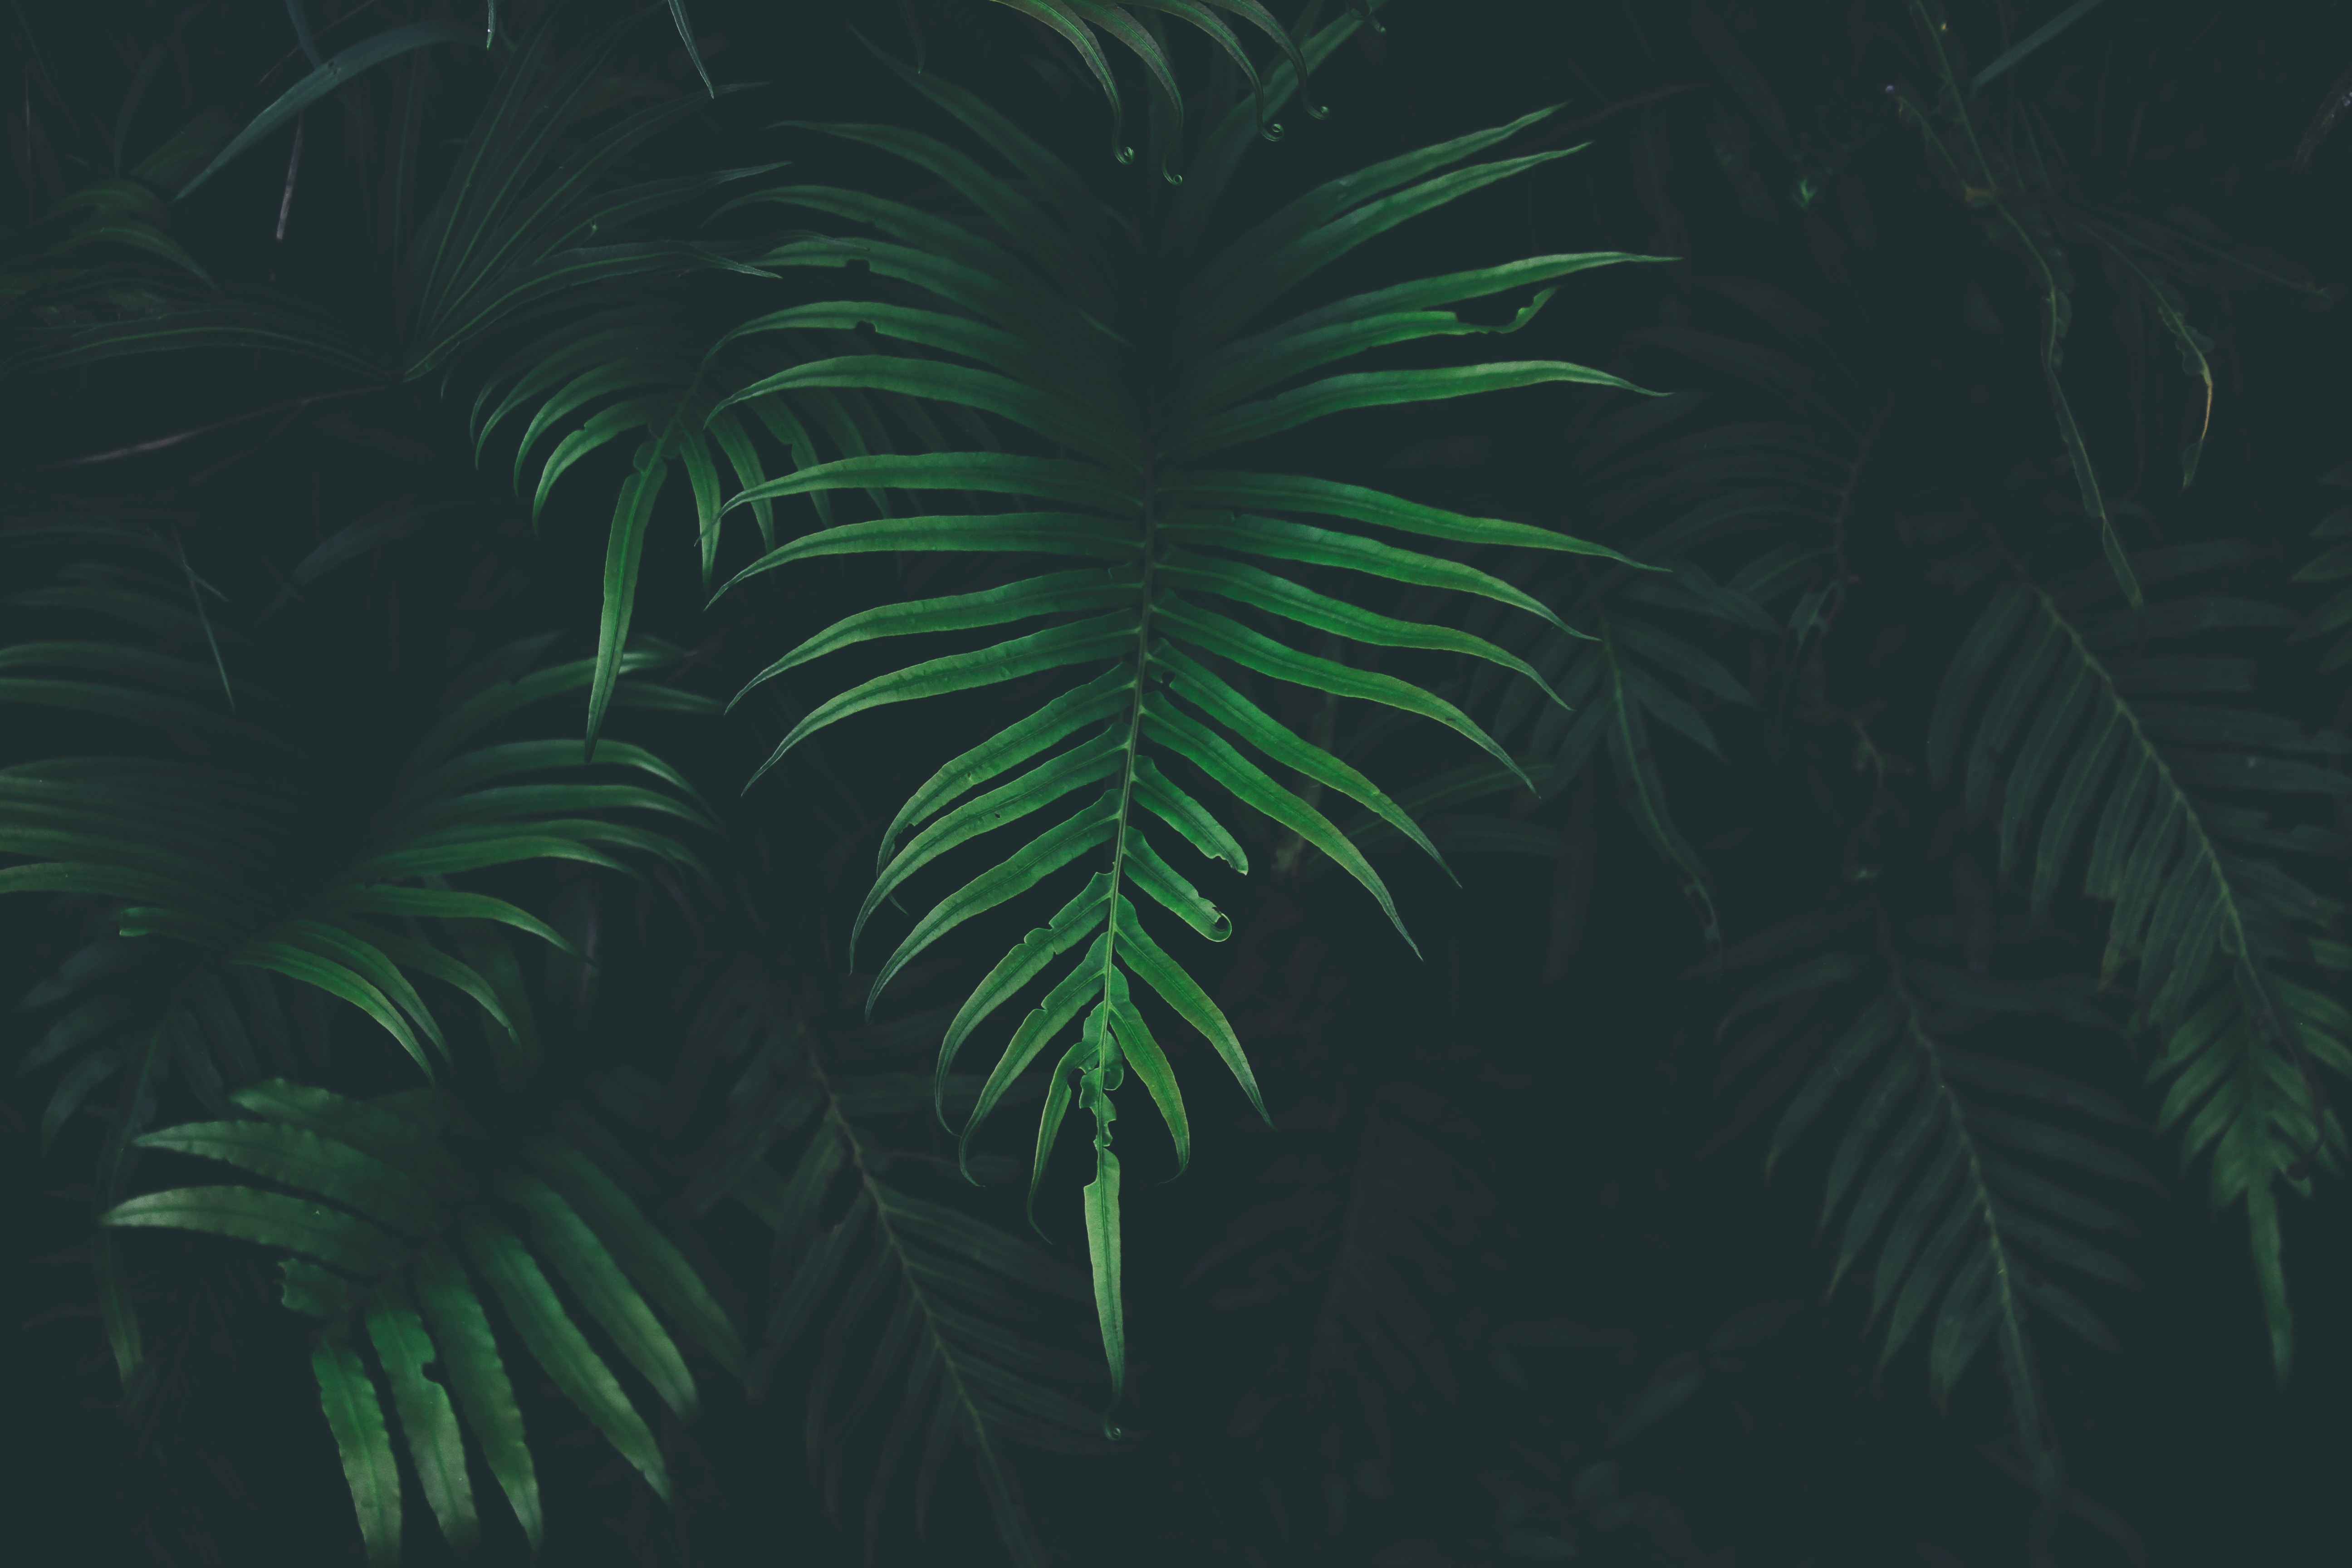
\includegraphics[width=1\textwidth]{image1.jpg}}
\end{center}

\chapter{Image 2}
\label{app:appendix2}

Lorem ipsum dolor sit amet, consectetur adipiscing elit. Nam a orci ornare nibh tincidunt molestie sed nec tellus. Morbi non sapien id lorem posuere pretium. Vestibulum commodo cursus purus, a elementum sem imperdiet sit amet.

\begin{center}
	\makebox[1\textwidth]{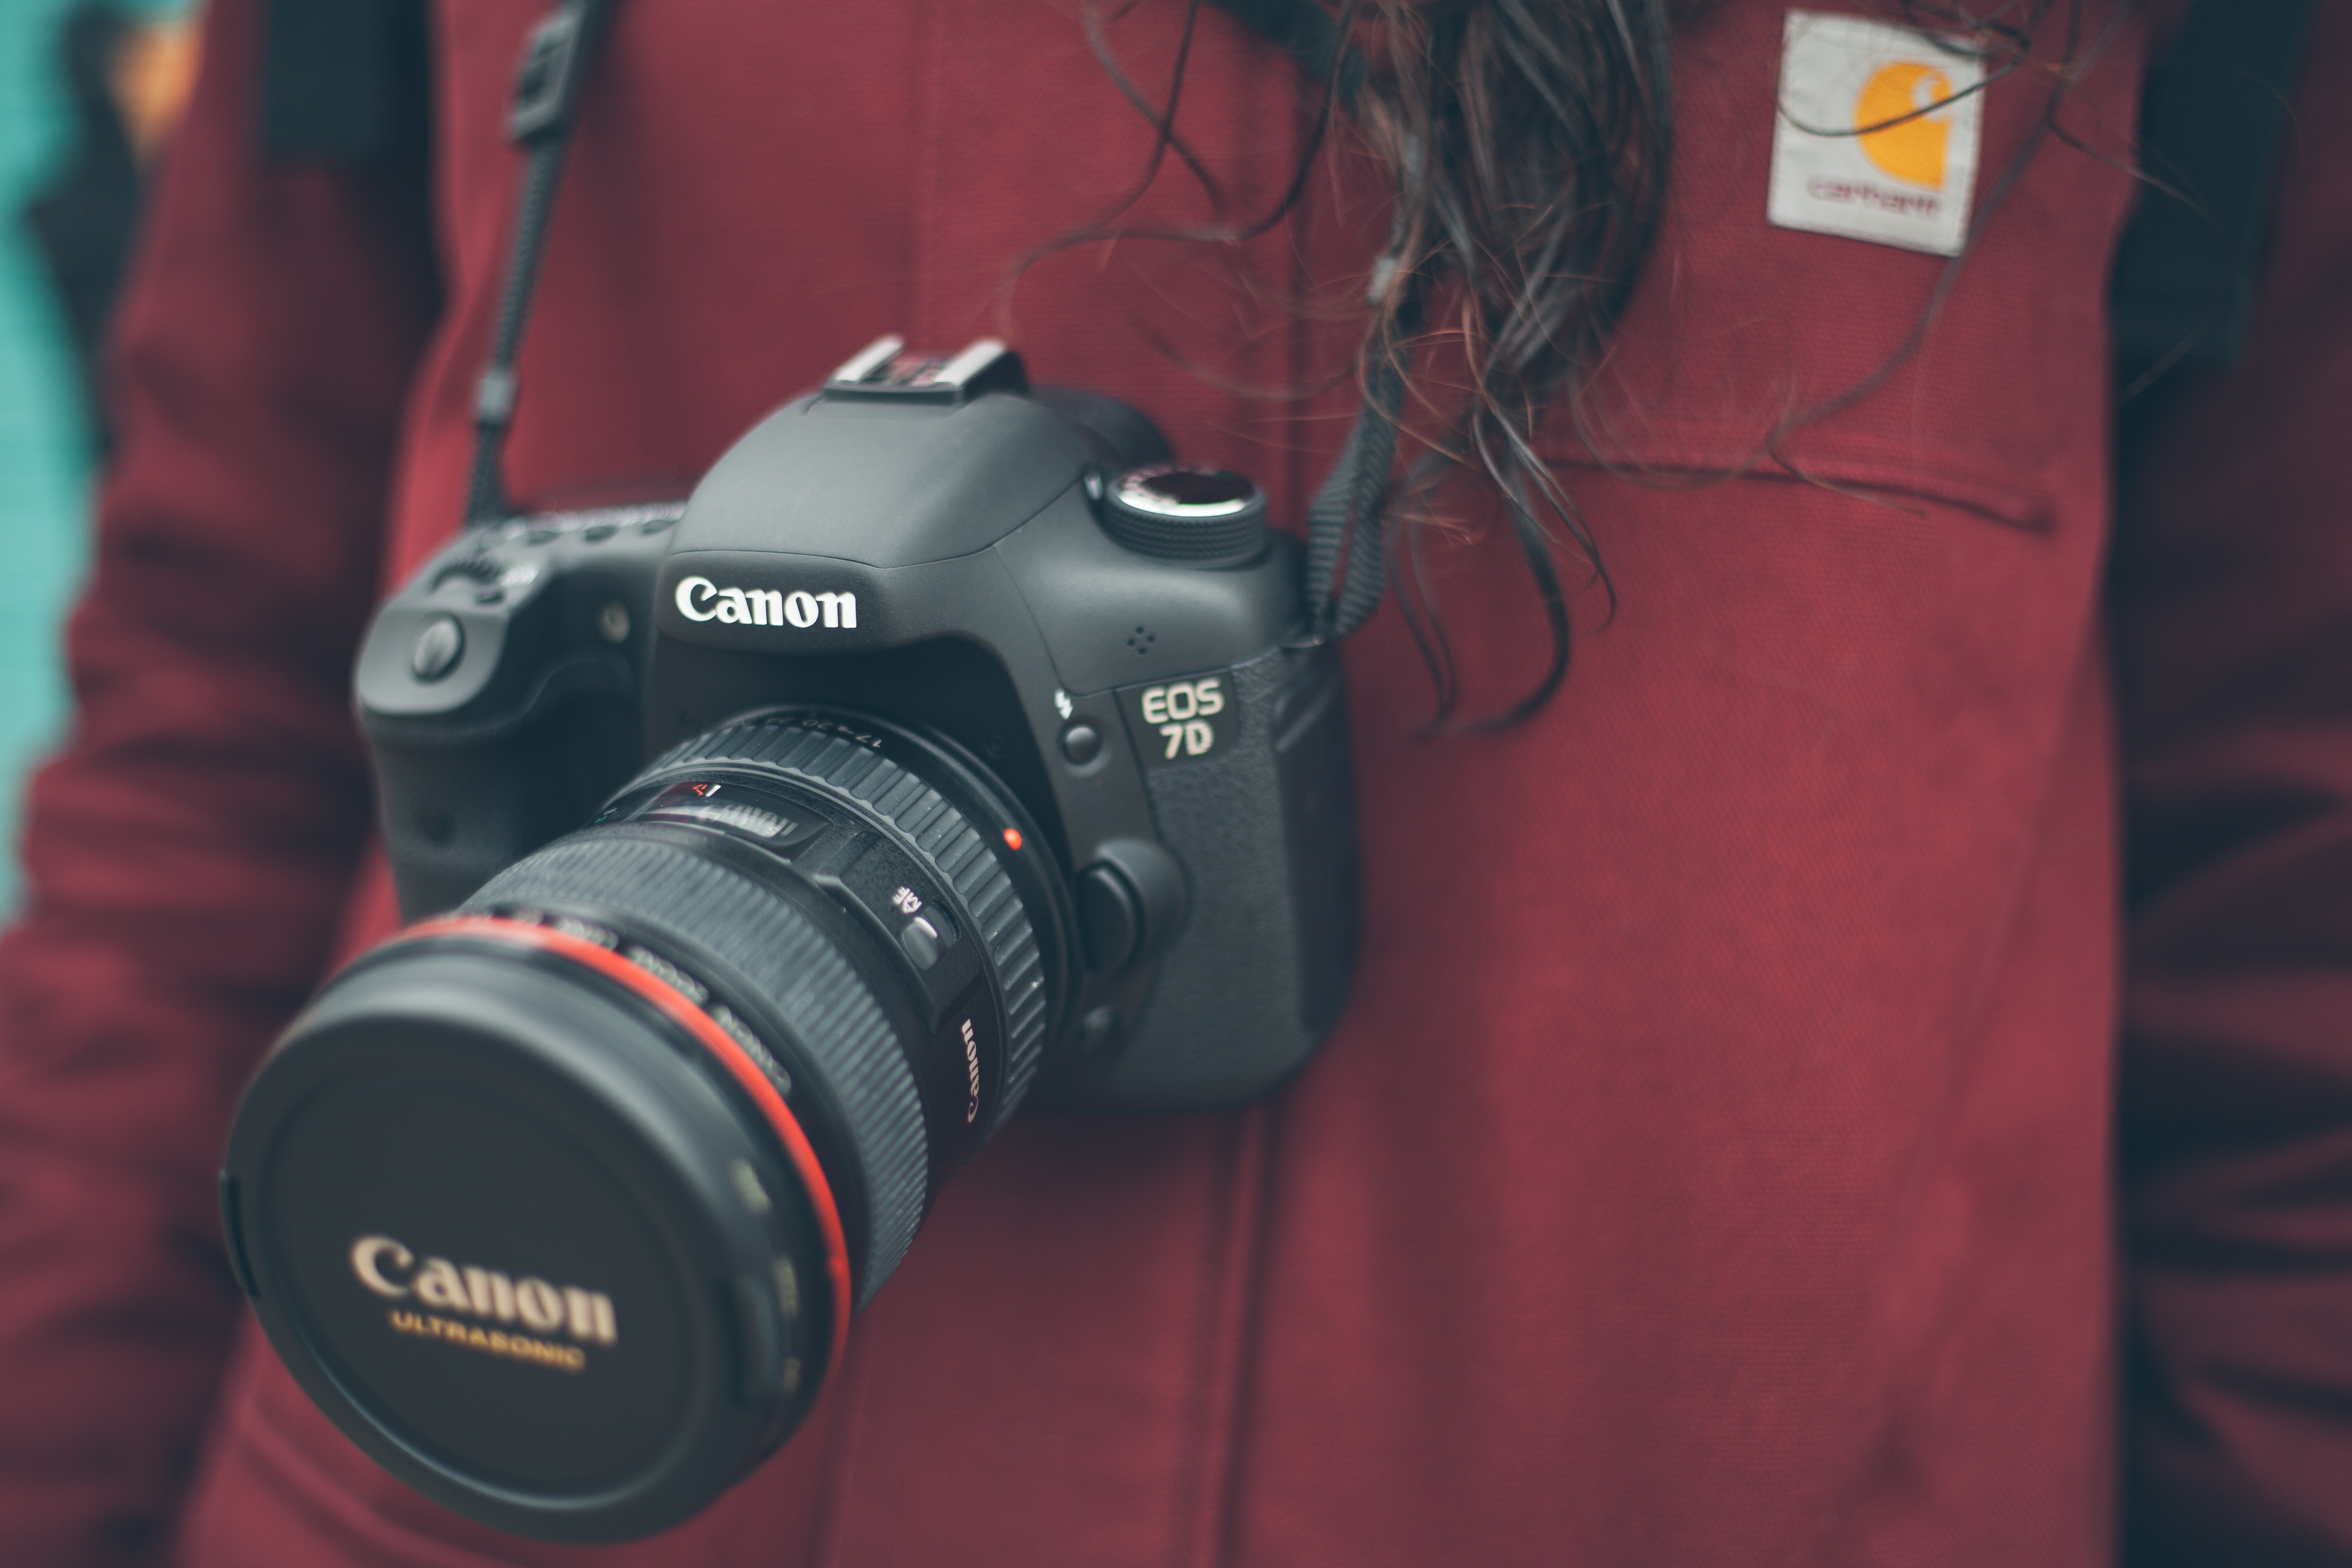
\includegraphics[width=1\textwidth]{image2.jpg}}
\end{center}


\end{appendices}
 % Anhänge

\end{document}